% REMEMBER: You must not plagiarise anything in your report. Be extremely careful.
\documentclass{l4proj}

    
%==============================================================================
% Put any additional packages here
% You can add any packages you want, as long as it does not alter
% the overall format (e.g. don't change the margins or the reference style).
%
\usepackage{pdfpages} % if you want to include a PDF for an ethics checklist, for example
\usepackage{tikz}
\usepackage{rotating}
\usepackage{amsmath}
\usepackage[normalem]{ulem}
\usepackage{lscape}
\usepackage{longtable}
\useunder{\uline}{\ul}{}
\usetikzlibrary{shapes.geometric, arrows, positioning, calc}
\tikzstyle{textblock} = [draw, minimum height=10mm, minimum width=20mm, align=center]
\tikzstyle{vertbox} = [inner sep=0, outer sep=0]
\tikzstyle{arrow} = [thick,->,>=stealth]
\tikzstyle{line} = [thick]
%
%

% commands
\newcommand{\tikzverticaltext}[1]{
    \begin{tikzpicture}
        \node[draw, minimum height=5mm, minimum width=40mm, align=center, anchor=center, rotate=90] {#1};
    \end{tikzpicture}
}

\begin{document}

%==============================================================================
%% METADATA
\title{Identifying Patterns of Tumour Tissue Architecture with Deep Representation Learning} % change this to your title
\author{Jetanat Sihanatkathakul}
\date{Febuary 5, 2025}

\maketitle

%==============================================================================
%% ABSTRACT
\begin{abstract}
    Histopathology serves as a critical tool for cancer diagnosis, with Haematoxylin and Eosin (H\&E) stained slides being the most frequently examined due to their versatility. This project builds upon the recently developed Histomorphological Phenotype Learning (HPL) methodology by \cite{ClaudioQuiros2024} to explore various deep learning architectures for analysing H\&E stained whole slide images (WSIs) and individual tile images.
    
   To classify WSIs, several classifier architectures were implemented, including multiple multilayer perceptron models and a logistic regression model. Evaluation revealed consistent performance across all architectures, though generally mediocre. A significant drop in performance was observed when models were applied to data from sources different from their training data, indicating limited generalisability between sources. Further investigation uncovered important limitations in using vector representations derived from cluster presentation proportions for cancer classification, as well as the adverse effect of training the classification models exclusively on primary tumour WSIs. 
   
   To create a lung cancer tile image captioning model, a novel workflow was proposed for creating tile-annotation pairings by utilising HPL methodology. The tile captioning model trained on these pairings showed promising results, with evaluation metrics indicating close similarity between generated and reference captions. This model serves as a proof of concept, demonstrating that a supervised learning approach could effectively train models with tile-level objectives using a dataset produced by the proposed workflow.
\end{abstract}

%==============================================================================
%% ACKNOWLEDGEMENTS
\chapter*{Acknowledgements}
% Enter any acknowledgements here. This is optional; you may leave this blank if you wish,
% or remove the entire chapter
%
% We give thanks to the Gods of LaTeX, who in their eternal graciousness, 
% have granted that this document may compile without errors or overfull hboxes.
%

My deepest gratitude to Ke Yuan, the supervisor of this project, for your magnificent guidance. This project succeeded in no small part because of you.

I would like to also thank Adalberto Claudio Quiros for his work on the HPL paper, which is the basis of this project. Your help with the HPL data and code is greatly appreciated.

%==============================================================================

% EDUCATION REUSE CONSENT FORM
% If you consent to your project being shown to future students for educational purposes
% then insert your name and the date below to  sign the education use form that appears in the front of the document. 
% You must explicitly give consent if you wish to do so.
% If you sign, your project may be included in the Hall of Fame if it scores particularly highly.
%
% Please note that you are under no obligation to sign 
% this declaration, but doing so would help future students.
%
\def\consentname {Jetanat Sihanatkathakul} % your full name
\def\consentdate {05 Febuary 2025} % the date you agree
%
\educationalconsent


%==============================================================================
\tableofcontents

%==============================================================================
%% Notes on formatting
%==============================================================================
% The first page, abstract and table of contents are numbered using Roman numerals and are not
% included in the page count. 
%
% From now on pages are numbered
% using Arabic numerals. Therefore, immediately after the first call to \chapter we need the call
% \pagenumbering{arabic} and this should be called once only in the document. 
%
%
% The first Chapter should then be on page 1. 

% PAGE LIMITS
% You are allowed 40 pages for a 40 credit project and 30 pages for a 
% 20 credit report. 
% This includes everything numbered in Arabic numerals (excluding front matter) up
% to but *excluding the appendices and bibliography*.
%
% FORMATTING
% You must not alter text size (it is currently 10pt) or alter margins or spacing.
% Do not alter the bibliography style. 
%
%==================================================================================================================================
%
% IMPORTANT
% The chapter headings and structure here are **suggestions**. You don't have to follow this model if
% it doesn't fit your project. Every project should have an introduction and conclusion,
% however.  If in doubt, your supervisor can give you specific guidance; their view takes precedence over
% the structure suggested here.
%
%==================================================================================================================================
\chapter{Introduction}

% reset page numbering. Don't remove this!
\pagenumbering{arabic} 

\section{To Diagnose Cancer}

Work-up for cancer diagnosis starts when the physician suspects that the patient may have cancer, for example from the patient's symptoms, medical history, or screening tests. Histopathology serves as a cornerstone diagnostic methodology in this process \citep{cancerNIH}. The procedure involves extracting tissue samples from a suspected tumour region, mounting them on slides, and applying appropriate preparation techniques. 

Slide preparation includes staining the slide to increase contrast, with one of the most common stains being Haematoxylin and Eosin (H\&E) \citep{Morrison2022}. Following preparation, histopathologists conduct detailed microscopic examinations of tissue morphology, yielding a trove of diagnostic information, including:
\begin{itemize}
    \item whether the tumour is malignant or benign
    \item the type (and sub-type) of the cancer
    \item the cancer grading.
\end{itemize}
This information is returned in a histological report, and is vital for diagnosis, prognosis, and treatment of cancer. Enhancement in histopathological methods and technologies to detect cancer will enhance our capabilities to combat it.

This project studies various deep learning architectures that use H\&E stained slide images as input. The aim is to use these models to improve cancer diagnosis from tissue images. There are two parts to this project:
\begin{enumerate}
    \item given a tissue slide, \emph{classify} it to the correct cancer type
    \item given a tissue tile image, \emph{caption} it with an appropriate description.
\end{enumerate}

\section{Whole Slide Image and Its Anatomy} \label{sec:WSI_anatomy}
The digital image of the prepared tissue slide, called a \emph{whole slide image (WSI)}, is obtained by putting the slide into a slide scanner. These WSIs contain the entirety of the slide at a particular magnification of the objective lens, typically 20x. The scanned images are often downsampled to lower magnifications, like 10x and 5x, and stored together in the WSI file \citep{Zarella2018}. 

While the digitised WSIs allow AI applications in histopathology, there are several distinct and unique challenges. WSIs are often too big, reaching multiple gigabytes in size, and contain too much data, up to gigapixels, to be used for training directly. Therefore, most successful models break the WSI up into tiles, and these tiles are then used to train the model. If the goal of the model is at a higher level than the tile-level (e.g., patient-level or slide-level), then the output from tiles will be aggregated to create a higher-level label \citep{Dimitriou2019}. Henceforth, this dissertation will refer to the broken up images from a WSI as \emph{tiles}. 

While the slide-level labels are widely available, models are usually not trained on the WSI directly. Labelling on each individual tile is expensive and labour-intensive. This poses a challenge to direct supervised learning algorithms, which require direct labels. Researchers circumvent this by using weakly supervised learning algorithms which only need weak labels, or have GUI tools for histopathologists to mark regions to increase labeling efficiency \citep{komura2018}.

In this study, two different approaches are utilised to deal with WSIs:
\begin{enumerate}
    \item Use self-supervised model to classify tissue tiles to clusters. The deep representation of a WSI is constructed from the proportions of clusters present in the slide.
    \item Use a new workflow to create a tile-level label. A model is trained on tiles, which now have direct labels, with a supervised learning algorithm to create a caption appropriate for each individual tile.
\end{enumerate}

WSIs come in many shapes and forms, but the ones significant to this project are the bright-field H\&E stained WSIs of tumour slides. These are available in public databases in Slide and Viewable Storage (SVS) files. This project uses SVS files from the following sources:
\begin{itemize}
    \item The Cancer Genome Atlas (TCGA) Research Network: \url{https://www.cancer.gov/tcga}
    \item Clinical Proteomic Tumor Analysis Consortium (CPTAC): \url{https://pdc.cancer.gov}
    \item The Cancer Moonshot Biobank (CMB): \url{https://moonshotbiobank.cancer.gov}
    \item The Genotype-Tissue Expression (GTEx) Project: \url{http://gtexportal.org}
\end{itemize}

Different sources use different names and abbreviations to refer to a particular type of cancer slide. This study follows TCGA's names and abbreviations. Likewise, primary sites for cancer types are referenced in the TCGA datasets. Details on names, primary sites, and associated datasets from these sources can be seen in Table \ref{tab:abbreviation}. Unlike other sources, GTEx provides physiological tissue slides, in which there is no cancer. Therefore, samples in the GTEx dataset will be separated by the primary sites instead. 

\begin{table}[]
\caption{Reference table for names and abbreviations. This project follows TCGA's abbreviation, seen in the Abbreviation column. Full TCGA dataset names can be seen in the Corresponding Datasets column, along with CMB and CPTAC datasets that belong to the same category. Primary site follows corresponding TCGA dataset. For example, BLCA primary site follows the site listed by TCGA-BLCA dataset.}
\label{tab:abbreviation}
\rowcolors{2}{}{gray!3}
\begin{tabular}{@{}p{0.05\linewidth}p{0.3\linewidth}p{0.15\linewidth}p{0.2\linewidth}p{0.2\linewidth}@{}}
% \toprule
\textbf{Index} & \textbf{Name}                                 & \textbf{Abbreviation} & \textbf{Primary Site(s)}              & \textbf{Corresponding Datasets} \\ \midrule
0     & Bladder Urothelial Carcinoma         & BLCA         & Bladder                      & TCGA-BLCA              \\
1     & Breast Invasive Carcinoma            & BRCA         & Breats                       & TCGA-BRCA, CMB-BRCA    \\
2     & Cervical Squamous Cell Carcinoma, Endocervical Adenocarcinoma & CESC & Cervix uteri & TCGA-CESC             \\
3     & Colon Adenocarcinoma                 & COAD         & Colon, Rectosigmoid Junction & TCGA-COAD, CPTAC-COAD  \\
4     & Lung Adenocarcinoma                  & LUAD         & Bronchus, Lung               & TCGA-LUAD, CPTAC-LUAD  \\
5     & Lung Squamous Cell Carcinoma         & LUSC         & Bronchus, Lung               & TCGA-LUSC, CPTAC-LSCC  \\
6     & Prostate Adenocarcinoma              & PRAD         & Prostate Gland               & TCGA-PRAD, CMB-PCA     \\
7     & Skin Cutaneous Melanoma              & SKCM         & Skin                         & TCGA-SKCM, CPTAC-CM    \\
8     & Stomach Adenocarcinoma               & STAD         & Stomach                      & TCGA-STAD              \\
9     & Uterine Corpus Endometrial Carcinoma & UCEC         & Corpus uteri                 & TCGA-UCEC, CPTAC-UCEC  \\ 
% \bottomrule
\end{tabular}
\end{table}

\section{Goals}
This project aims to answer two research questions:
\begin{enumerate}
    \item How effectively can a model that utilises deep representations of whole slide images presented in the Histomorphological Phenotype Learning (HPL) methodology classify cancerous WSIs to the correct cancer type?

    \item How can tile-level annotations be generated, and can these annotations be used to train a model that produces descriptive captions for lung cancer tiles?

\end{enumerate}

Exploring the first question, we evaluated the utility of WSI vectors from the HPL methodology for cancer type classification. A number of classifier models were implemented and assessed on multiple datasets. Chapter \ref{sec:WSI} covers this question, including the classifier architectures, the training process, and the metrics on the models' performances on these datasets.

Chapter \ref{sec:caption} focuses on the second question. It elaborates on the specifics of the workflow used to create tile-annotation pairings, the process to create the tile image captioning model, and the model's evaluation using automated metrics.

The discussions on each research question are provided in their respective chapters along with the results. They assume the background knowledge outlined in Chapter \ref{sec:background}, particularly Section \ref{sec:HPL} about the HPL methodology foundational to this project.

%==================================================================================================================================
\chapter{Background} \label{sec:background}

\section{DeepPATH Framework} \label{sec:deeppath}
To deal with the enormous size of WSI files, they need to be split up into tiles. DeepPATH is an approach to classifying lung histology samples into normal, adenocarcinoma, and squamous cell carcinoma samples by introduced \cite{Coudray2018}. WSIs in SVS format are processed with DeepPATH, and the output is an HDF5\footnote{https://www.hdfgroup.org/solutions/hdf5/} file containing separate tissue tiles and their metadata. Tiles that contain background areas over a certain threshold percentage are also filtered out.

We used this framework to tile WSIs and perform stain normalisation. It was also used for packing images with metadata in neat HDF5 files.

\section{Histomorphological Phenotype Learning} \label{sec:HPL}
Histomorphological Phenotype Learning (HPL) methodology was proposed in a recent paper by \cite{ClaudioQuiros2024}. The study recognised problems and limitations of applying supervised learning to a histopathology problem: primarily that it is limited by the available data, and it is subject to human bias. HPL utilises self-supervised learning to train the backbone tissue tile image encoder, and uses clustering to identify visually similar tissue tiles. The process is illustrated in Figure \ref{fig:HPL}.

\begin{figure}
    \centering
    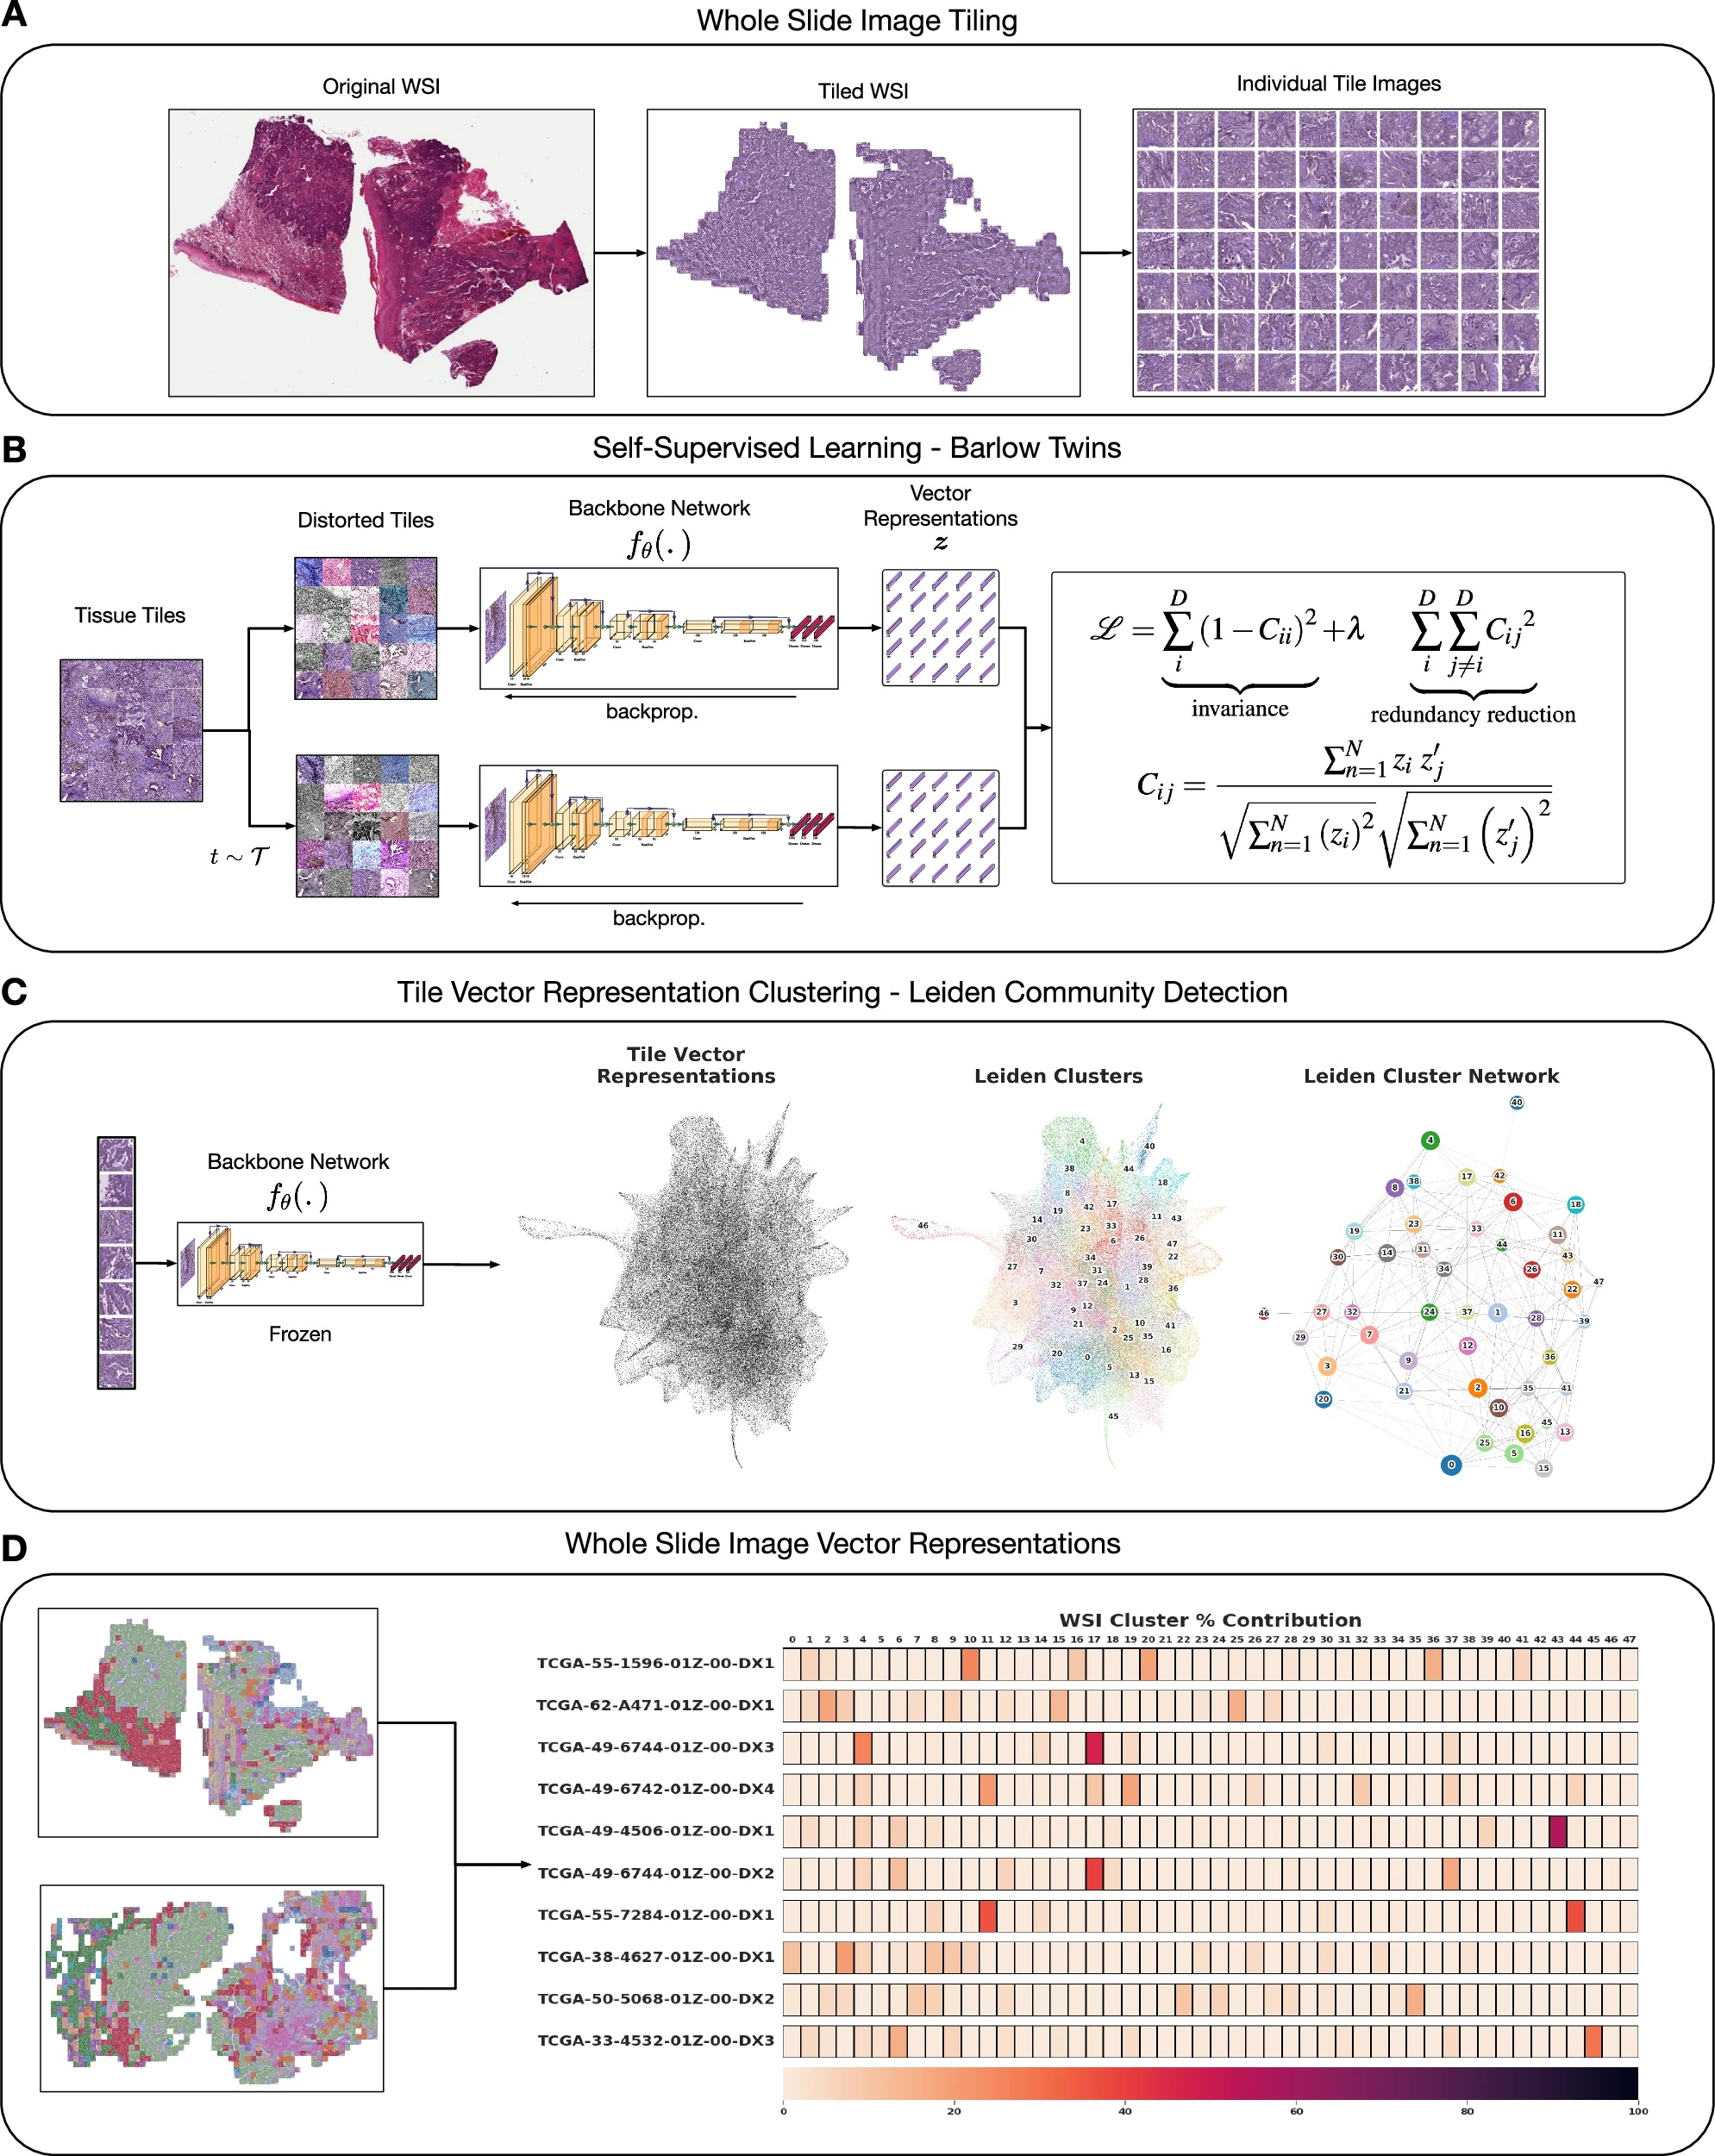
\includegraphics[width=1\linewidth]{images/HPL.png.jpg}
    \caption{Illustration of the full HPL methodology. A: WSI tiling and stain normalisation process using DeepPATH framework. B: training of CNN tile image encoder using self-supervised algorithm, Barlow Twins. C: clustering tile image representation vectors (z-vectors) using Leiden Community Detection. D: creating WSI vector from constituent clusters that make up the slide. Image from \cite{ClaudioQuiros2024}.}
    \label{fig:HPL}
\end{figure}

The methodology uses the same DeepPATH tiling algorithm mentioned in Section \ref{sec:deeppath}. The tiles are fed to a convolutional neural network (CNN), composed of ResNet layers \citep{resnet} and one self-attention layer. This backbone network is trained using Barlow Twins, a self-supervised learning algorithm \citep{zbontar2021}. The network is frozen and acts as an encoder to extract features from the tissue tile images. The output from the CNN backbone network is a length-128 vector for each tissue tile, which will be referred to later as a \emph{z-vector} ($\boldsymbol{z} \in \mathbb{R}^{128}$). In addition to the z-vector, a length-1024 vector, called \emph{h-vector} ($\boldsymbol{h} \in \mathbb{R}^{1024}$), which is the vector before the final fully connected layers in the CNN model, is also available in the HPL methodology.

The z-vectors are treated as representations of tissue tiles. Clustering is performed on the representations to group visually similar tiles into the same clusters. A community detection algorithm, known as the Leiden Community Detection algorithm \citep{Traag2019}, is used to cluster z-vectors. The clusters or communities from this algorithm are referred to as Histomorphological Phenotype Clusters (HPC).

The study used percentages of HPCs inside a WSI assembled as a vector to represent the WSI. The final representation of a WSI is called a \emph{WSI vector}.

To create a WSI vector, each component tissue tile is fed through the backbone network, giving a z-vector, and clustered, giving the HPC that the tile belongs to. The frequency of each HPC in the WSI is counted, and it constitutes each element in the vector, giving a vector of HPC frequencies. The vector is then normalised using a centered log-ratio transformation. The vector of frequencies of HPCs frequently had zero elements, resulting in the geometric mean of $0$. To avoid that, a constant is added to all elements in the vector to impute zeroes. With $g(\boldsymbol{v})$ as the geometric mean after zero imputation with a constant $c$:
\begin{equation}
    g(\boldsymbol{v}) = \left( \prod_{i=0}^{C-1} v_i + c\ \right)^\frac{1}{C} ,
\end{equation}
\begin{equation}
    \boldsymbol{w} = \left[log\frac{v_0 + c}{g(\boldsymbol{v})},log\frac{v_1 + c}{g(\boldsymbol{v})},\dots,log\frac{v_{C-1} + c}{g(\boldsymbol{v})}\right],
\end{equation}
with $\boldsymbol{v}$ being the composite vector of cluster frequencies, $C$ the number of HPCs (equals to the length of the vector), and $\boldsymbol{w}$ being the WSI vector. HPL code uses $c = 1$, so we used the same value.

The HPL study used two different datasets: the TCGA lung dataset, comprising 2 lung cancer subtypes from TCGA, and the TCGA pancancer dataset, comprising 10 different cancer types or subtypes. For the TCGA lung dataset, in addition to clustering and creating vector representation as above, the HPCs produced by the process were annotated by multiple expert pathologists, giving textual information describing each HPC. 

This study concerns three different parts in the HPL paper:
\begin{itemize}
    \item We treated \emph{WSI vectors} as representations of their original WSIs. Models were built and trained to classify these vectors into the correct cancer type of the original WSI.
    \item \emph{Pathologist annotations of lung HPCs} were used to create tissue tile and annotation pairings. The tile images belonging to a HPC inherited the annotation from the cluster. This allowed us to train a supervised model for tile image captioning.
    \item We treated the backbone model as a pre-trained image encoder and the output vectors (\emph{z-vectors} and \emph{h-vectors}) were the representations of their original tile images.
\end{itemize}

\section{SHapley Additive exPlanations}
SHapley Additive exPlanations (SHAP)\footnote{https://shap.readthedocs.io/en/latest/} is a framework presented in a paper by \cite{lundberg2017}. Simple models, like logistic regression models, can be investigated by looking at the parameters of the model to understand how the model calculates the output. As the complexity of the model increases, it becomes exponentially more difficult to reason about the model. SHAP framework attempts to explain the model's inner mechanisms by using cooperative game theory.

Each individual element of the input vector is assigned a contribution score, called SHAP value. SHAP values are assigned by the framework using fair allocation in cooperative game theory \citep{Szymaski2025}. The features are the players in the game, and the model is the rule of the game. The formulation:
\begin{equation}
    E[f(z)\ |\ do(z_S = x_S)],
\end{equation}
where $S$ is a subset of the features, $x$ is a data sample, is used to evaluate the effect of a subset of feature inputs on the output of the model $f(x)$ \citep{ShapDoc}. Figure \ref{fig:shap} illustrates the effect of SHAP values ($\phi_i$) on the expected model output, and the additive nature of SHAP values.

Features with high SHAP value magnitudes are considered to have more significant impacts on the model's prediction. We used SHAP values to explain models and to investigate particular values that have high (positive) impacts on the predictions for some classes.

\begin{figure}
    \centering
    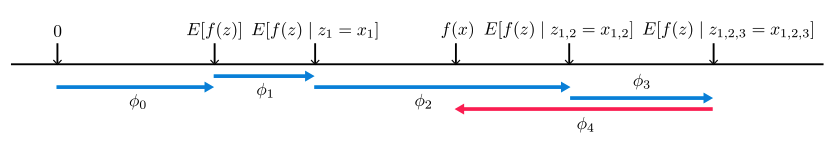
\includegraphics[width=1\linewidth]{images/shap.png}
    \caption{Effect of SHAP values of each feature on the model output conditioned on subsets of features. $\phi_0$ is the base value which is the expectation of the model output without any known input. Image from \cite{lundberg2017}.}
    \label{fig:shap}
\end{figure}

\section{CNN-RNN Architecture}
A study by \cite{Vinyals2015} proposed a neural network architecture to generate general descriptions from an image. The model uses a deep vision CNN as an image encoder, followed by a language-generating network. The CNN encoder produces an information-rich representation vector of the image, which is the input to the language decoder. The sentence generation model in the study is a type of recurrent neural network (RNN), known as Long Short-Term Memory (LSTM), which is explained in more detail in Section \ref{sec:LSTM}.

This architecture produced state-of-the-art results at the time of its publication for image captioning tasks. However, multiple newer model architectures have been published in more recent papers that boast better results. Examples include mPLUG \citep{mplug}, GIT \citep{GIT}, and BLIP-2 \citep{blip2}. While the image encoder has largely remained the same over the years, using CNNs. There have been developments in the language decoder section, such as using transformers or other attention-based models. 

The CNN-RNN architecture is an older architecture compared to the attention-based ones. Nevertheless, it should produce decent results for this study. The data for the tile image captioning task was derived from one instance of clustering and annotating by pathologists. As a result, the captions for the images were not very diverse. There were as many variations of captions as the number of lung HPCs, which was 46. This small pool of reference captions made the task markedly easier than datasets generally used for benchmarking, such as COCO Captions\footnote{https://cocodataset.org/} or nocaps\footnote{https://nocaps.org}. The tile image captioning model in this study follows the CNN-RNN architecture.

%==================================================================================================================================
\section{Neural Network Components}
This section describes the components of the models in this project. It introduces concepts, terminologies, and notations that are used in this paper.

\subsection{Linear/Fully Connected Layer}
A linear layer, also called a fully connected layer, is a layer that calculates the linear combination of its inputs and adds a constant, called bias, to it. The linear layer \emph{fully connects} each and every input to all outputs via a linear combination as follows:
\begin{equation}
    Linear(\boldsymbol{x}) = \boldsymbol{x} \boldsymbol{A}^T + \boldsymbol{b},
\end{equation}
where $\boldsymbol{x}$ is the input, $\boldsymbol{A}$ is the weight matrix, and $\boldsymbol{b}$ is the bias.

The linear layer is one of the most basic blocks in deep learning. It is used ubiquitously as stand-alone layers in all models involved in this project and as components of more complex layers.

\subsection{Rectified Linear Unit}
A rectified linear unit (ReLU) layer applies the element-wise rectifier function to the inputs. Mathematically, this is defined as:
\begin{equation}
    \text{ReLU}(\boldsymbol{x})_i = \max(0, x_i) = 
    \begin{cases}
        x_i & \text{if} \ x_i > 0 \\
        0 & \text{if} \ x_i \leq 0
    \end{cases}
    \ ,
\end{equation}
where subscripts (e.g., $x_i$) refer to the $i^{th}$ element of the vector.

Activation functions are used to introduce non-linearity to the model. We utilised non-linearity to push the MLP model's classification power above that of the logistic regression model. ReLU is a popular choice for an activation function due to its simplicity in computation, both forward and backward. It is also non-saturating, which is preferred over saturating counterparts like hyperbolic tangent or sigmoid. This is because non-saturating functions like ReLU suffer less from the vanishing gradient problem, allowing it to support larger models and make models train faster \citep{glorot2011, krizhevsky2017}.

Because of the aforementioned properties, ReLU was the activation function of choice for this project. The classifiers involved with the first research question use only either the vanilla version of the ReLU function or its leaky version.

\subsection{Leaky Rectified Linear Unit} \label{sec:LeakyReLU}
Very similarly to ReLU, a leaky rectified linear unit (leaky ReLU) is its leaky variant and is defined by the following element-wise function:
\begin{equation}
    \text{LeakyReLU}(\boldsymbol{x})_i = \max(\alpha x_i, x_i) = 
    \begin{cases}
        x_i & \text{if} \ x_i > 0 \\
        \alpha x_i & \text{if} \ x_i \leq 0
    \end{cases}
    \ ,
\end{equation}
where $\alpha$ is some constant in the range $(0, 1)$ sometimes referred to as the negative slope.

One problem with using ReLU is that the gradient for the negative region is $0$. This can lead to a problem known as the \emph{dying ReLU problem}. A neuron can always output $0$ given any inputs, and this can lead to the neuron dying, as it has no chance to learn because of the zero gradient \citep{Lu2020}. Leaky ReLU allows a small gradient in the negative region, which mitigates the dying ReLU problem. The gradient in the positive region is $1$, while $\alpha$ defines the gradient in the negative region. Mathematically, this is:
\begin{equation}
    \text{LeakyReLU}'(\boldsymbol{x})_i = 
    \begin{cases}
        1 & \text{if} \ x_i > 0 \\
        \alpha & \text{if} \ x_i \leq 0
    \end{cases} \ .
\end{equation}

It was shown in a study by \cite{xu2015} that training a model with Leaky ReLU could provide better model performance than doing so with normal ReLU. Therefore, we experimented with additional variants of the classifier which utilise leaky ReLU functions in place of ReLU functions, aiming to improve the classification ability.

\subsection{Dropout} \label{sec:dropout}
Overfitting is a fundamental challenge in machine learning applications. The data used to train a model constitutes only a sample of the entire population to which the model will be applied. This sampling noise can be a source of inaccuracy. Models trained on limited data samples may perform exceptionally well on the training data but generalise poorly on unseen data.

Regularisations are implemented to mitigate overfitting,  with dropout regularisation being particularly prevalent. Dropout silences some units in the neural network with a predetermined probability during the training phase. This concept can be formalised to equations:
\begin{equation}
    r_i \sim \text{Bernoulli}(1-p),
\end{equation}
\begin{equation}
    \text{Dropout}(\boldsymbol{x})_i = r_ix_i \cdot \frac{1}{1-p},
\end{equation}
where $p \in [0,1]$ is the dropout probability. The $\frac{1}{1-p}$ term is added to scale the output during training, so the expected value of the output remains consistent between training and inferencing phases. 

This deactivation only applies when the model is in the training state. This prevents neurons from excessively adapting to each other. At test time or running time, all units will be present (i.e. $p = 0$), and the dropout function is just the identity function. 

This method has been shown by \cite{srivastava2014} to be an effective way of improving performance in various model architectures and applications, while also reducing overfitting. We implemented dropout regularisation for classifier models for the first question as separate variants, intending to attain these benefits.

\subsection{Softmax Function}
Output of a linear layer or either flavour of ReLU is unbounded and cannot be directly interpreted as a probabilistic distribution. Instead, the output is treated as a vector of logits, which can be transformed into a probability distribution by applying the softmax function. It is mathematically defined as:
\begin{equation}
    \text{Softmax}(\boldsymbol{x})_i = \frac{e^{x_i}}{\sum\limits^{N}_{j=1}e^{x_j}},
\end{equation}
where $N$ denotes the length of the input (and output) vector.

Each element of the output from the softmax function is bounded within the range $(0, 1)$, and the vector satisfies the property:
\begin{equation}
    \sum\limits_{i=1}^N \text{Softmax}(\boldsymbol{x})_i = 1.
\end{equation} 
Therefore, the output from the softmax function can be directly interpreted as a probability distribution over the classes.

The models in this project do not use the softmax function explicitly, as it is included as a package inside the cross-entropy loss function. This is elaborated in the very next section.

\subsection{Cross-Entropy Loss}
We employed the cross-entropy function as the loss function for model training. Cross-entropy loss is defined as the mean of the multiclass cross-entropy across all data samples:
\begin{equation}
    \mathcal{L} = -\frac{1}{N} \left( \sum_{i=1}^N \sum_{c=1}^C y_{i, c} \log p_{i, c} \right),
\end{equation}
where $N$ is the number of data samples, $C$ is the number of classes, $y_{i,c}$ is the true probability of the $i^{th}$ sample being class $c$ ($1$ for the correct class and $0$ otherwise), and $p_{i,c}$ is the model's predicted probability that the $i^{th}$ sample belongs to class $c$.

This function quantifies the difference between the model's predicted probability distribution and the true distribution. Models are optimised to minimise this difference. Cross-entropy loss is widely used for classification tasks, making it ideal for the first research question, which is to classify WSIs into appropriate cancer classes. Additionally, it is extended for the second question of generating captions for tissue tiles.

We used \verb|nn.CrossEntropyLoss| from PyTorch\footnote{https://pytorch.org} which combines softmax and cross-entropy (referred to as negative log-likelihood in the PyTorch context). The loss for each individual data sample is calculated as:
\begin{equation}\label{eq:cross-entropy-loss}
    \text{CrossEntropyLoss}(\boldsymbol{x}, \boldsymbol{y}) = \sum_{c=1}^C y_{c} \log \frac{e^{x_c}}{\sum\limits^{N}_{j=1}e^{x_j}}\ ,
\end{equation}
with $C$ being the total number of classes, $y_c$ the true probability of the sample being class $c$, and $x_c$ the predicted probability from the model of the sample being class $c$.

To address class imbalances in the dataset, we also employed \emph{weighted} cross-entropy loss, in which a weight term is augmented to the cross-entropy function in Equation \ref{eq:cross-entropy-loss} as follows:
\begin{equation}
    \text{WeightedCrossEntropyLoss}(\boldsymbol{x}, \boldsymbol{y}) = \sum_{c=1}^C w_c y_{c} \log \frac{e^{x_c}}{\sum\limits^{N}_{j=1}e^{x_j}}\ ,
\end{equation}

where $w_c$ is the weight for class $c$.

Weighted cross-entropy loss allows additional control over the training process by telling the model to pay more or less attention to samples from different classes. High weights can be assigned to under-represented classes to compensate for the low number of samples in the training data, effectively increasing the importance of each individual sample. This is particularly relevant to the first research question, where there were significant imbalances between classes in the dataset.


\subsection{Embedding Layer} \label{sec:embedding-layer}
Neural networks require numerical data for processing and cannot handle strings directly. Therefore, the captions associated with tile image captioning must be converted to numerical representations. The tile captioning model uses text embedding, a process which transforms each individual text token into an embedding vector. Consequently, a complete sentence is represented by a tensor comprising multiple word embedding vectors. The full embedding process is illustrated in Figure \ref{fig:embedding-process}. 

We used the \verb|nn.Embedding| module from PyTorch to encode a vector of token indices into a tensor of embeddings. Documentation on the module can be found at \url{https://pytorch.org/docs/stable/generated/torch.nn.Embedding.html}.

For clarity and simplicity in model diagrams, the \emph{embedding layer} refers specifically to a layer that transforms a word token, like `fibrotic', into its corresponding embedding vector. This is illustrated in Figure \ref{fig:embedding-layer}.

\begin{figure}[h!]
    \centering
    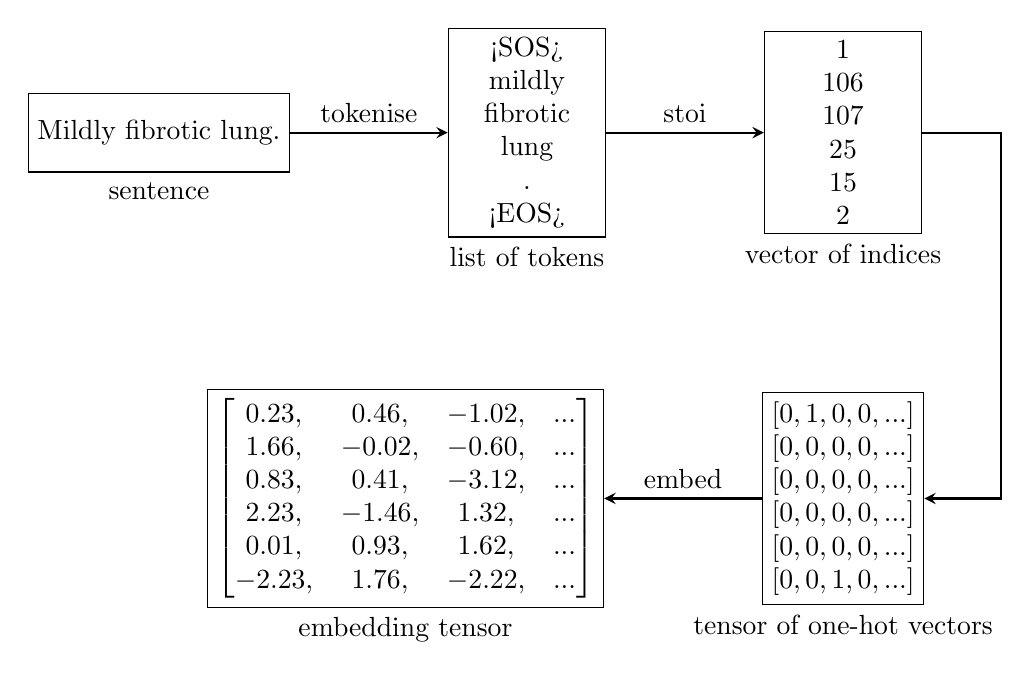
\begin{tikzpicture}
        
        % Input Text
        \node[textblock] (input) {Mildly fibrotic lung.};
        \node[below=0mm of input] {sentence};

        % Token Nodes
        \node[textblock, right=20mm of input] (token) {<SOS>\\mildly\\fibrotic\\lung\\.\\<EOS>};
        \node[below=0mm of token] {list of tokens};

        % 
        \node[textblock, right=20mm of token] (indices) {1\\106\\107\\25\\15\\2};
        \node[below=0mm of indices] {vector of indices};

        %
        \node[textblock, below=20mm of indices] (onehot) {$[0, 1, 0, 0, ...]$ \\ $[0, 0, 0, 0, ...]$ \\ $[0, 0, 0, 0, ...]$ \\ $[0, 0, 0, 0, ...]$ \\ $[0, 0, 0, 0, ...]$ \\ $[0, 0, 1, 0, ...]$};
        \node[below=0mm of onehot] {tensor of one-hot vectors};

        \node[textblock, left=20mm of onehot] (embeddings) {$
            \begin{bmatrix}
                0.23,&0.46,&-1.02,&... \\
                1.66,&-0.02,&-0.60,&... \\
                0.83,&0.41,&-3.12,&... \\
                2.23,&-1.46,&1.32,&... \\
                0.01,&0.93,&1.62,&... \\
                -2.23,&1.76,&-2.22,&...
            \end{bmatrix}
            $};
        \node[below=0mm of embeddings] {embedding tensor};
        
        % Arrows
        \draw[arrow] (input) -- (token)
        node[midway, above] {tokenise};
        \draw[arrow] (token) -- (indices)
        node[midway, above] {stoi};
        \draw[arrow] (indices.east) |- ($(indices.east) + (1,0)$) |- (onehot.east);
        \draw[arrow] (onehot) -- (embeddings)
        node[midway, above] {embed};
    \end{tikzpicture}
    \caption{Diagram illustrating the complete process of transforming a sentence from a string into a tensor of word embedding vectors. The example phrase ``Mildly fibrotic lung.'' undergoes tokenisation, vocabulary mapping, and embedding transformation. <SOS> and <EOS> represent the special tokens for the start and end of a sequence, respectively. stoi denotes the string-to-index transformation.}
    \label{fig:embedding-process}
\end{figure}

\begin{figure}[h!]
    \centering
    \begin{tikzpicture}
        \node[textblock] (token) {fibrotic};
        \node[vertbox, right=20mm of token] (embeddinglayer) {\tikzverticaltext{Embedding Layer}};
        \node[textblock, right=20mm of embeddinglayer] (embedding) {$[0.83, 0.41, -3.12, ...]$};

        \draw[line] (token) -- (embeddinglayer);
        \draw[arrow] (embeddinglayer) -- (embedding);
    \end{tikzpicture}
    \caption{Diagram illustrating the behaviour of the embedding layer. The token representing the word ``fibrotic'' is being transformed by the embedding layer, producing its corresponding embedding vector.}
    \label{fig:embedding-layer}
\end{figure}

\subsection{Long Short-Term Memory Architecture} \label{sec:LSTM}
Recurrent neural networks (RNNs) are specialised neural network architectures that excel at processing sequential data, including text. Unlike normal feedforward networks, RNNs have the ability to process data in cycles, maintaining internal states to integrate information across multiple timesteps \citep{Schmidt2019RecurrentNN}. In other words, the output at timestep $t$ depends on not only the current input at $t$, but also the inputs from previous timesteps $(0 \dots t-1)$. 

The problem with conventional RNNs is that the error either explodes or diminishes exponentially with an increasing number of timesteps. Long-short term memory architecture (LSTM) solves the vanishing and exploding gradient problems by maintaining a constant error flow \citep{lstm1997}. The central design to support this idea is called a constant error carousel (CEC).

History from previous cycles, which is the cell state in the LSTM context, flows freely through time via the carousel. The state is only accessible through special gates: the forget gate and the input gate \citep{LSTMolah}.

The forget gate decides whether to squash the memory from the previous cell state ($c_{t-1}$) based on the latest input ($\boldsymbol{x_t}$). Given that $\sigma$ is the sigmoid activation function:
\begin{equation}
    \sigma (\boldsymbol{x})_i = \frac{1+e^{x_i}}{e^{x_i}},
\end{equation}
the equation for the output of the forget gate is:
\begin{equation}
    \boldsymbol{f}_t = \sigma(\text{Linear}(\boldsymbol{x_t}) + \text{Linear}(\boldsymbol{h}_{t-1})),
\end{equation}
where $\boldsymbol{h}$ is called the hidden state of the LSTM memory cell. Subscripts $t$ denote values at time step $t$.

The other gate is the input gate, which represents remembering new things. The input gate has its own internal gate that determines whether the new information should be remembered or not. This is represented by this equation:
\begin{equation}
    \boldsymbol{i}_t = \sigma(\text{Linear}(\boldsymbol{x}_t) + \text{Linear}(\boldsymbol{h}_{t-1})).
\end{equation}

Another component determines which part of the input should be remembered. With $tanh$ referring to the hyperbolic tan activation function:
\begin{equation}
    \tanh(\boldsymbol{x})_i = \frac{e^{2x_i} - 1}{e^{2x_i} + 1}\ ,
\end{equation}
the equation for this part of the input gate is:
\begin{equation}
    \Tilde{\boldsymbol{c}}_t = \tanh(\text{Linear}(\boldsymbol{x}_t) + \text{Linear}(\boldsymbol{h}_{t-1})).
\end{equation}

The flow of the cell state through time for a memory cell is thus:
\begin{equation}
    \boldsymbol{c}_t = \boldsymbol{f}_t \odot \boldsymbol{c}_{t-1} + \boldsymbol{i}_t \odot \Tilde{\boldsymbol{c}}_t,
\end{equation}
where $\odot$ denotes element-wise product.

The hidden state ($\boldsymbol{h}$) is used as the output of the LSTM cell. The output cell state is passed through a $tanh$ activation function and squashed through the output gate ($\boldsymbol{o}$) to get the hidden state for the cell:
\begin{equation}
    \boldsymbol{o}_t = \sigma(\text{Linear}(\boldsymbol{x}_t) + \text{Linear}(\boldsymbol{h}_{t-1})),
\end{equation}
\begin{equation}
    \boldsymbol{h}_t = \tanh(\boldsymbol{c}_t) \odot \boldsymbol{o}_t.
\end{equation}

We used the LSTM implementation in the PyTorch library, as \verb|nn.LSTM| module. Its documentation is accessible at \url{https://pytorch.org/docs/stable/generated/torch.nn.LSTM.html}. The LSTM architecture is a component of the tile captioning model implemented as part of the investigation into the second research question. 

%==================================================================================================================================

\section{Metrics} \label{sec:metrics}
This section describes the metrics used for model evaluation. The following abbreviations are used throughout the equations in this section:
\begin{itemize}
    \item $TP$: True Positive
    \item $TN$: True Negative
    \item $FP$: False Positive
    \item $FN$: False Negative
    \item $N$: Number of samples
    \item $C$: Number of classes.
\end{itemize}

The abbreviations above will be extended to the class-specific context as follows:
\begin{itemize}
    \item $TP_c$: True Positive for class $c$; the number of samples in class $c$ that are correctly classified as class $c$.
    \item $FP_c$: False Positive for class $c$; the number of samples not in class $c$ that are classified as class $c$.
    \item $FN_c$: False Negative for class $c$; the number of samples in class $c$ that are incorrectly classified as some other class.
\end{itemize}



\subsection{Accuracy} \label{sec:accuracy-metric}
The accuracy metric shows the proportion of samples classified correctly, normalised by the total number of samples:

\begin{equation} \label{eq:microacc}
    \text{Accuracy} = \frac{1}{N} \sum_{i=1}^{N}\boldsymbol{1}(y_i = \hat{y}_i) =  \frac{TP+TN}{N}\ ,
\end{equation}
where $y_i$ denotes the true class of the $i^{th}$ sample, $\hat{y_i}$ represents its corresponding prediction, and $\boldsymbol{1}(x)$ is the indicator function that evaluates to $1$ when the condition is true and $0$ otherwise.

We also used top-k accuracy metric. It follows similar principles with a modified notion of correctness. For top-k accuracies, a prediction is considered \emph{correct} if the true class appears among the $k$ highest ranked predictions. For example, top-1 accuracy is exactly as stated in Equation \ref{eq:microacc}. Top-3 accuracy considers a prediction correct if the true class is predicted as the most, second-most, or third-most likely class. This metric is formalised mathematically as follows:

\begin{equation}
    \text{Top-$k$ Accuracy} = \frac{1}{N} \sum_{i=1}^{N} \sum_{j=1}^k \boldsymbol{1}(y_i = \hat{f}_{i,j})\ ,
\end{equation}
where $\hat{f}_{i,j}$ corresponds to the class with $j^{th}$ highest prediction score for the $i^{th}$ sample.

Additionally, we also employed per-class accuracy or class-specific accuracy. For this metric, only samples belonging to a certain class are included in the calculation. Per-class equivalent of Equation \ref{eq:microacc} is:
\begin{equation} \label{eq:macroacc}
    \text{Class-m Accuracy} = \frac{1}{|S_m|} \sum_{y_s \in S_m}\boldsymbol{1}(y_s = \hat{y}_s),
\end{equation}
where $S_m$ denotes the set containing all samples with the label $m$.

We used the overall accuracy to evaluate the cancer type classifiers, which shows the general picture, along with top-3 and top-5 accuracies, which offer more insight into the predictions in relation to the ground truth. Per-class accuracy is useful for a more fine-grained examination and is more appropriate in cases where there are classes missing from the evaluation dataset.

While the accuracy metric is informative, it has several pitfalls, one of which is the sensitivity to class imbalances in the dataset. Therefore, we considered other metrics along with, such as the F1 score, to ensure a more comprehensive assessment of model performance.

\subsection{Recall, Precision, and F1 Score} \label{sec:F1-score}
We used macro-averaged values of recall, precision, and F1 score to evaluate the classifiers. Macro-averaging means that the metrics are calculated for each class separately; then the overall average is calculated. These metrics are defined by the following equations:
\begin{equation}
    \text{Recall} = \frac{1}{C}\sum_{c=1}^{C}\frac{TP_c}{TP_c + FN_c}\ ,
\end{equation}
\begin{equation}
    \text{Precision} = \frac{1}{C}\sum_{c=1}^{C}\frac{TP_c}{TP_c+FP_c}\ ,
\end{equation}
\begin{equation}\label{eq:f1}
    \text{F}_1 = \frac{1}{C}\sum_{c=1}^{C}\frac{2 \times TP_c}{2 \times (TP_c + FP_c + FN_c)}\ .
\end{equation}

In this dissertation, macro F1 score is the arithmetic mean of the class-specific F1 scores, where each class-specific F1 score is the harmonic mean of class-specific precision and recall \citep{opitz2021}. The Equation \ref{eq:f1} is equivalent to:
\begin{equation}
    \text{F}_1 = \frac{1}{C}\sum_{c=1}^{C}2 \times \frac{\text{Precision}_c \times \text{Recall}_c}{\text{Precision}_c + \text{Recall}_c}\ ,
\end{equation}
where Recall$_c$ and Precision$_c$ denote class $c$ specific recall and precision, respectively.

Recall captures how well the model is capturing a particular class, and precision captures how specific the positive predictions are. In other words, recall is maximised when the model minimises false negatives, whereas precision is maximised when the model minimises false positives. F1 score offers a balanced metric between recall and precision when there is no preference between the two.


\subsection{Receiver Operating Characteristic (ROC) Curve}
Receiver Operating Characteristic (ROC) curve is a graphical representation of how well the model distinguishes between classes. In this study, the ROC curves are plotted using the one-vs-rest approach, whereby for each class, the samples belonging to that particular class are designated as positive instances and others as negative instances.

ROC curve visualises the performance of the classification model, by showing its prediction across multiple decision thresholds. Moving rightward along the graph corresponds to decreasing the decision threshold. As the threshold decreases, the model identifies more positive samples correctly, but simultaneously classifies more negative samples incorrectly as positive. In a one-vs-rest context, this means that while the model identifies more instances of a particular class, it also erroneously assigns that class label to samples from other classes. Classifiers with superior performances are characterised by ROC curves that approach the top-left corner of the graph.

Since the proximity of the ROC curve to the top-left corner indicates a good model, this quality can be quantified by the area under the ROC curve (henceforth also referred to as AUROC). AUROC is a common metric for comparing the performances of multiple model architectures. The AUROC value is bound within $[0, 1]$, with higher values indicating superior model capability to differentiate patterns in the data into appropriate classes.

While other metrics like accuracy and F1 score only consider the final predictions by the model, the AUROC incorporates the output probabilities from the model. We used AUROC values to quantify the model's ability to differentiate between classes. They were used to evaluate the performance of cancer type classifiers and the effectiveness of different classifier variants.

\subsection{Confusion Matrix}
Visualising a model's classification behaviour across different classes provides valuable diagnostic information. This visualisation is achieved through a confusion matrix. In this representation, each row corresponds to samples of a particular true class, while each column represents the model's prediction for a specific class. The cell at an intersection between row $i$ and column $j$ quantifies the proportion of samples of class $i$ that the model classifies as belonging to class $j$.

Given this definition, a good model have high values on the main diagonal line, where $i = j$. Beyond that, confusion matrices reveal systematic misclassification patterns. For instance, they reveal whether a model is consistently misclassifying one particular class as another. We used the confusion matrix for conducting in-depth analyses of the predictions by the cancer classifier models.

The matrices presented in this dissertation are normalised by row. Specifically, the value in the cell at row $i$ and column $j$ is the portion of samples in class $i$ that are classified as class $j$. Consequently, values in each row sum up to $1$, unless the dataset contains no sample of a particular class. In such case, all cells in the corresponding row are $0$. The equation for each cell value is calculated as:
\begin{equation}
    c_{i,j} = \frac{z_{i, j}}{\sum\limits_{k=1}^C z_{i,k}},
\end{equation}
where $c_{i,j}$ denotes the value of the cell at row $i$ column $j$, and $z_{i,j}$ represents the number of class $i$ samples that the model predicts as class $j$.

\subsection{\textsc{Rouge}}
Recall-Oriented Understudy for Gisting Evaluation or \textsc{Rouge} is an automatic evaluation framework for natural language processing (NLP) tasks, originally proposed by \cite{lin2004} for evaluating automated text summarisation. Traditionally, this is analogous to the recall of the text model: measuring how much of the reference text is captured in the model's output. The implementation by Google\footnote{https://github.com/google-research/google-research/tree/master/rouge} includes the precision and F1 variant of the metric as well. This study reports recall, precision, and F1 score for \textsc{Rouge}, with primary emphasis on the traditional recall variant. Throughout this dissertation, \textsc{Rouge} \emph{score} always specifically refers to recall.

\textsc{Rouge-N} is an n-gram variant of the metric. For instance, \textsc{Rouge-1} utilises unigrams (1-grams) for evaluation. \textsc{Rouge-N} score is defined as an n-gram recall between the candidate output sentence and the reference sentence. With $G_n(a)$ being the set of n-grams in sentence $a$, and $C(s, b)$ being the number of occurrences of n-gram $s$ in $b$:
\begin{equation}
\begin{split}    
    \textsc{Rouge-N}_{\text{recall}} &= \frac{\sum\limits_{s \in G_n(\text{Ref})}\min\left( C(s, \text{Ref}), C(s, \text{Cnd})\right)}{\sum\limits_{g \in G_n(\text{Ref})}C(s, \text{Ref})} \\
    &= \frac{\text{Number of overlapping N-grams}}{\text{Total number of N-grams in the reference}}\ ,
\end{split}
\end{equation}
where Cnd represents the candidate sentence (model prediction), and Ref denotes the reference sentence (ground truth).

The precision variant uses the same idea but is defined as an n-gram precision. The equation is largely the same, with one major difference in the denominator being swapped for n-grams in the candidate text:
\begin{equation}
\begin{split}    
    \textsc{Rouge-N}_{\text{precision}} &= \frac{\sum\limits_{s \in G_n(\text{Cnd})}\min\left( C(s, \text{Ref}), C(s, \text{Cnd})\right)}{\sum\limits_{g \in G_n(\text{Cnd})}C(s, \text{Cnd})} \\
    &= \frac{\text{Number of overlapping N-grams}}{\text{Total number of N-grams in the candidate}}\ .
\end{split}
\end{equation}

The \textsc{Rouge-N} F1 score is the harmonic mean of its recall and precision variants:
\begin{equation}
    \textsc{Rouge-N}_{\text{F1}} = 2 \times \frac{\textsc{Rouge-N}_{\text{recall}} \times \textsc{Rouge-N}_{\text{precision}}}{\textsc{Rouge-N}_\text{recall} + \textsc{Rouge-N}_\text{precision}}\ .
\end{equation}

\textsc{Rouge-L} calculates the similarity between the candidate and the reference by finding the longest common subsequence between two sequences of words or tokens. This is defined as:
\begin{equation}
    \textsc{Rouge-L}_\text{recall} = \frac{\text{LCS}(\text{Cnd}, \text{Ref})}{\text{len}(\text{Ref})},
\end{equation}
\begin{equation}
    \textsc{Rouge-L}_{\text{precision}} = \frac{\text{LCS}(\text{Cnd}, \text{Ref})}{\text{len}(\text{Cnd})},
\end{equation}
\begin{equation}
    \textsc{Rouge-L}_{\text{F1}} = 2 \times \frac{\textsc{Rouge-L}_\text{recall} \times \textsc{Rouge-L}_\text{precision}}{\textsc{Rouge-L}_\text{recall} + \textsc{Rouge-L}_\text{precision}}\ ,
\end{equation}
where LCS$($Cnd$,$ Ref$)$ is the length of the longest common subsequence between the candidate and the reference texts, and len$(x)$ represents the number of words in the text $x$.

For evaluating short single-sentence texts, \textsc{Rouge-L} is the most commonly used metric, while the original paper also recommends \textsc{Rouge-1}. To comprehensively assess the tile captioning models, we evaluated them using \textsc{Rouge-L}, \textsc{Rouge-1}, and also \textsc{Rouge-2} scores from the \textsc{Rouge} framework.

\subsection{\textsc{Bleu}}
In contrast to \textsc{Rouge}, BiLingual Evaluation Understudy (\textsc{Bleu}) is a precision-oriented metric. \textsc{Bleu} was introduced by \cite{papineni2002} as an automated evaluation framework for machine translation systems. The score quantifies the precision of the candidate text relative to the reference text.
\textsc{Bleu} employs a concept called modified n-gram precision, or clipped n-gram precision ($p_n$). This functions similarly to \textsc{Rouge} precision:
\begin{equation}
    p_n = \frac{\sum\limits_{s \in G_n(\text{Cnd})}\min\left( C(s, \text{Ref}), C(s, \text{Cnd})\right)}{\sum\limits_{g \in G_n(\text{Cnd})}C(s, \text{Cnd})}\ .
\end{equation}

Additionally, \textsc{Bleu} incorporates a brevity penalty ($Bp$) to penalise short sentences. The penalty reduces scores for outputs shorter than the reference text, while outputs equal to or longer in length than the reference are unaffected:
\begin{equation}
    Bp = 
    \begin{cases}
        1, & \text{if}\ \text{len}(\text{Cnd}) \geq \text{len}(\text{Ref}) \\
        e^{1-\frac{\text{len}(\text{Ref})}{\text{len}(\text{Cnd})}}, & \text{if}\ \text{len}(\text{Cnd}) < \text{len}(\text{Ref})
    \end{cases}
    .
\end{equation}

Relying on a single type of n-gram precision is not sufficiently robust. Therefore, the \textsc{Bleu} score takes into account multiple modified precision scores by finding the weighted geometric mean of multiple precisions. The formula for the \textsc{Bleu} score is:
\begin{equation}
\begin{split}
    \textsc{Bleu-N} &= Bp \cdot \prod_{n=1}^N p_n^{w_n} \\
                    &= Bp \cdot \exp\left(\sum_{n=1}^N w_n\log(p_n)\right),
\end{split}
\end{equation}
where $w_n$ is the weight value for n-gram modified precision. Conventionally, uniform weights are applied, such that $w_n = \frac{1}{N}$.

We used \textsc{Bleu-4} (sometimes called \textsc{Bleu@4}, \textsc{B@4} or \textsc{B-4}) for assessing the tile captioning models. Both \textsc{Rouge} and \textsc{Bleu} are reported as decimal values in the range of $[0, 1]$.

Both \textsc{Bleu} and \textsc{Rouge} share many similarities in their approaches to text evaluation. They both use n-grams in their metrics, as a way to reflect certain structures in the language. Both metrics exhibit certain limitations, including \citep{ananyaNLG}:
\begin{itemize}
    \item Both are very sensitive to tokenisation and/or normalisation methods. Difference in these can significantly affect the scores reported by these metrics. To ensure consistency, this study employs common tokenisation and normalisation procedures during both training and evaluation phases.
    \item Both only consider similarity at n-gram level. The metrics are not aware of similarity between semantics or other properties of the text. This may include synonyms or the actual meaning of the sentence.
\end{itemize}

For these metrics, scores are individually computed for each image, comparing the model's output as the candidate text against the ground truth caption, then averaged across the dataset to produce the final reported values.

%==================================================================================================================================
\chapter{Classifying Whole Slide Images of Cancer Tissues Using Their Deep Representations} \label{sec:WSI}

This chapter contains the answer to the first research question: how well WSIs can be classified based on their representations. We implemented classifiers utilising a deep representation of the WSI generated through the HPL methodology, called the WSI vector, for classification. The WSI vector creation process is detailed in Section \ref{sec:HPL}. The study encompasses 10 cancer types, which are enumerated in Table \ref{tab:abbreviation}.

Section \ref{sec:WSImodel} describes the architectures of the classification models employed. Section \ref{sec:WSItraining} elaborates on the training procedures for these models. The results from testing across a number of datasets are presented and discussed in Sections \ref{sec:5fold}, \ref{sec:external}, and \ref{sec:ood-results}. Finally, the overall findings are presented in Section \ref{sec:discuss-classifier}. 

\section{Models} \label{sec:WSImodel}
The first question addresses a multiclass classification problem. Several different classifier architectures were evaluated with baseline models including logistic regression and deep multilayer perceptron models. Both of these were simple feedforward networks. Figure \ref{fig:classifiers} provides a graphical representation of these model architectures and their variants.

\begin{figure}[] 
    \centering
    \begin{subfigure}[b]{0.3\textwidth}
        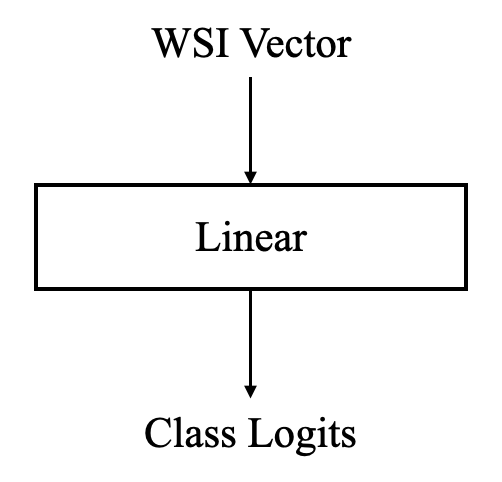
\includegraphics[width=\textwidth]{images/logreg.png}
        \caption{PanCancerLogisticRegression}
        \label{fig:logisticregression}
    \end{subfigure}
    \quad
    \begin{subfigure}[b]{0.3\textwidth}
        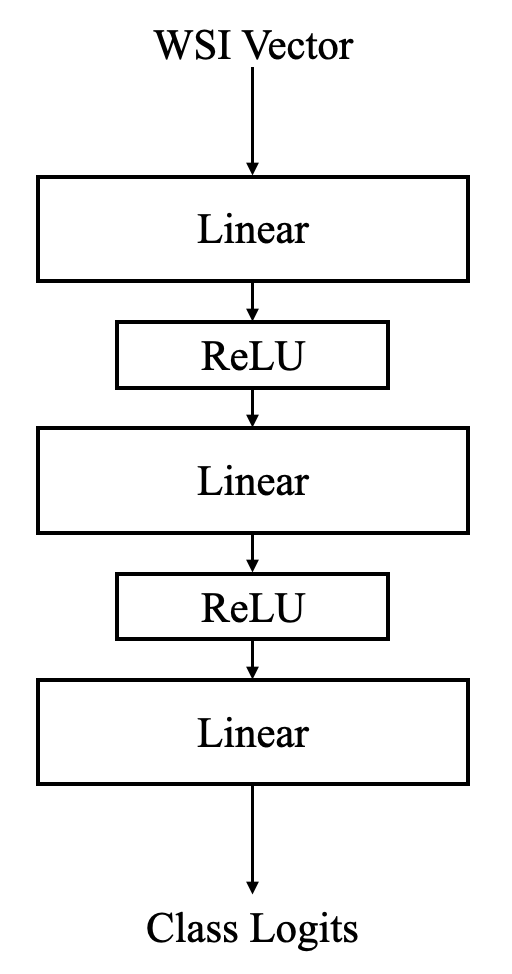
\includegraphics[width=\textwidth]{images/pancancerclassifier.png}
        \caption{PanCancerClassifier}
        \label{fig:pancancerclassifier}
    \end{subfigure}
    \quad
    \begin{subfigure}[b]{0.3\textwidth}
        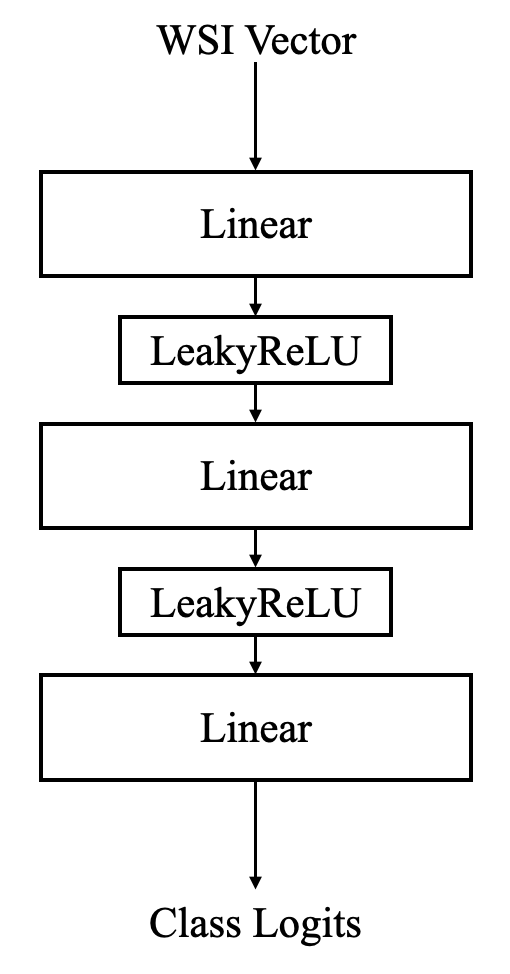
\includegraphics[width=\textwidth]{images/leakyclassifier.png}
        \caption{LeakyPanCancerClassifier}
        \label{fig:leakypancancerclassifier}
    \end{subfigure}
    \vfill
    \begin{subfigure}[b]{0.3\textwidth}
        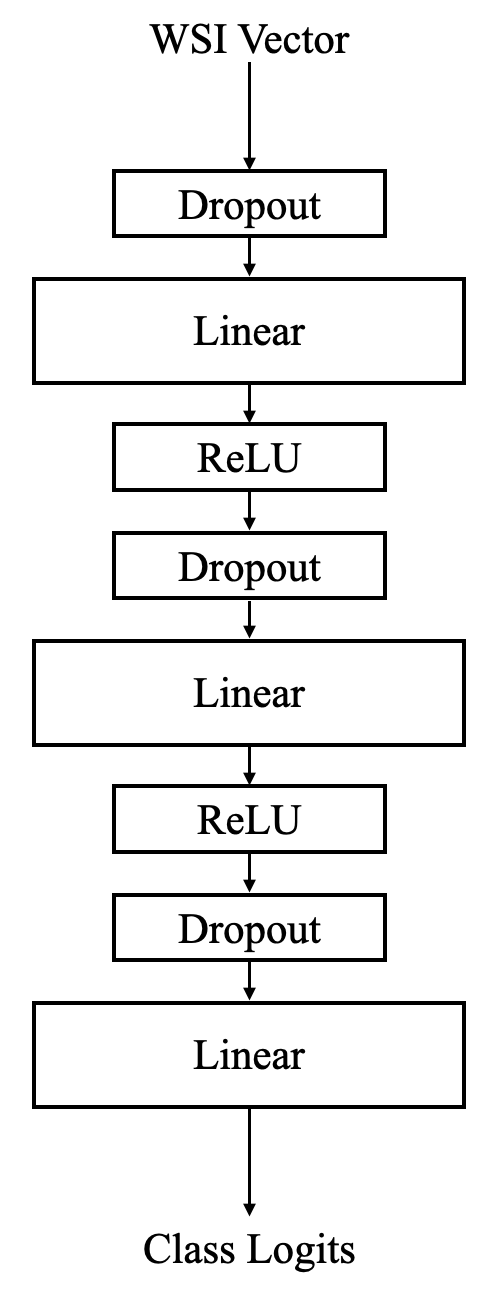
\includegraphics[width=\textwidth]{images/dropoutclassifier.png}
        \caption{PanCancerClassifierWithDropout}
        \label{fig:pancancerclassifierdropout}
    \end{subfigure}
    \quad
    \begin{subfigure}[b]{0.3\textwidth}
        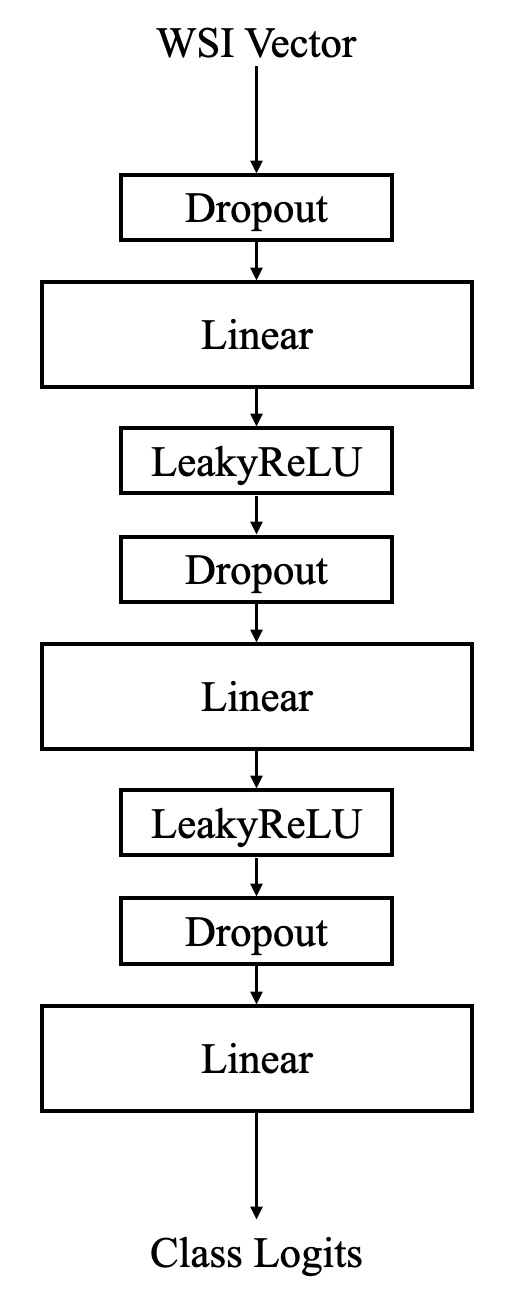
\includegraphics[width=\textwidth]{images/dropoutleakyclassifier.png}
        \caption{LeakyPanCancerClassifierWithDropout}
        \label{fig:leakypancancerclassifierdropout}
    \end{subfigure}
    \caption{Graphical representations of classifier architectures. The outputs of these models are raw unnormalised probabilities, also known as logits. \subref{fig:logisticregression} shows the logistic regression model, which is not a deep model as it consists only of one linear layer. \subref{fig:pancancerclassifier} and \subref{fig:leakypancancerclassifier} show the standard MLP variant, with 3 linear layers interspersed with activation functions. These models use ReLU and LeakyReLU as their activation functions respectively. \subref{fig:pancancerclassifierdropout} and \subref{fig:leakypancancerclassifierdropout} are their dropout counterparts.
    }\label{fig:classifiers}
\end{figure}

For all implemented models, softmax normalisation are deliberately omitted from the output layer. The outputs are treated as unnormalised prediction values (logits) rather than probabilistic values. The predicted class is determined by identifying the class with the highest logit value using the argmax function. Similarly, prediction ranking is accomplished by ordering logit values. The models are configured this way to increase numerical stability when calculating loss with \verb|nn.CrossEntropyLoss|.

Logistic regression (or softmax regression) model consists of only one fully connected layer. While logistic regression is simpler and has less classification power than the deep models, it offers the benefits of being easier to interpret by examining the model parameters directly, being less power and data hungry, and being less prone to overfitting. We implemented one of such, called \emph{PanCancerLogisticRegression}, represented by the equation:
\begin{equation}
    \text{PanCancerLogisticRegression}(\boldsymbol{x}) = \text{Linear}(\boldsymbol{x}).
\end{equation}

Multilayer perceptron (MLP) refers to feedforward networks with multiple fully connected layers interspersed with non-linear activation functions such as ReLU. Although more complex than logistic regression, MLPs offer more differentiation capabilities, especially for non-linearly separable data. The baseline model for MLP, \emph{PanCancerClassifier}, employs 3 linear layers with ReLU activation functions. It can be expressed as:
\begin{equation}
    \phi(\boldsymbol{x}) = \text{ReLU}(\text{Linear}(\boldsymbol{x})),
\end{equation}
\begin{equation}
    \text{PanCancerClassifier}(\boldsymbol{x}) = \text{Linear}(\phi(\phi(\boldsymbol{x}))).
\end{equation}

As discussed in Section \ref{sec:LeakyReLU}, the leaky variant of the ReLU may enhance model performance. Therefore, we implemented another MLP model which uses LeakyReLU instead of ReLU, designated as \emph{LeakyPanCancerClassifier}. It is determined by the following equations:
\begin{equation}
    \phi'(\boldsymbol{x}) = \text{LeakyReLU}(\text{Linear}(\boldsymbol{x})),
\end{equation}
\begin{equation}
    \text{LeakyPanCancerClassifier}(\boldsymbol{x}) = \text{Linear}(\phi'(\phi'(\boldsymbol{x}))).
\end{equation}

Finally, dropout regularisation (described in Section \ref{sec:dropout}) can mitigate overfitting and improve performance. We implemented dropout variants for both MLP architectures. These are called \emph{PanCancerClassifierWithDropout} and \emph{LeakyPanCancerClassifierWithDropout} for the ReLU and LeakyReLU variants respectively. These models incorporate dropout layers at the input and between neurons with a dropout probability of $0.2$. They are represented by the following equations:
\begin{equation}
    \phi_\text{drop}(\boldsymbol{x}) = \text{Dropout}(\text{ReLU}(\text{Linear}(\boldsymbol{x}))),
\end{equation}
\begin{equation}
    \text{PanCancerClassifierWithDropout}(\boldsymbol{x}) = \text{Linear}(\phi_\text{drop}(\phi_\text{drop}(\text{Dropout}(\boldsymbol{x})))),
\end{equation}

\begin{equation}
    \phi_\text{drop}'(\boldsymbol{x}) = \text{Dropout}(\text{LeakyReLU}(\text{Linear}(\boldsymbol{x}))),
\end{equation}
\begin{equation}
    \text{LeakyPanCancerClassifierWithDropout}(\boldsymbol{x}) = \text{Linear}(\phi_\text{drop}'(\phi_\text{drop}'(\text{Dropout}(\boldsymbol{x})))).
\end{equation}

\section{Training} \label{sec:WSItraining}
We used weighted cross-entropy loss as the loss function. Adam was used as the optimisation method, with a learning rate of $1e-3$. This configuration was applied to all classifier models. The models were trained for 30 epochs.

The weights for addressing class imbalance were calculated as follows:
\begin{equation}
    w_c = \frac{N}{n_c \cdot C}\ ,
\end{equation}
where $w_c$ is the weight for class $c$, $N$ is the total number of samples in the training set, $n_c$ is the number of samples of class $c$ in the training set, and $C$ is the number of classes. For this application with 10 types of cancer, $C = 10$.

This weighting scheme assigns higher importance to individual samples of under-represented classes. Without such weighting, the model might assign more samples to classes with more representation in the training set than it should, because they contribute more to the overall loss. This weighting mechanism prevents such a scenario by forcing each class to have equal importance, regardless of the number of samples in the training data.

Adam, short for Adaptive Moment Estimation, is an optimisation method belonging to the gradient descent family, introduced by \cite{kingma2017}. Adam has demonstrated faster convergence compared to other optimisers of the same family, such as stochastic gradient descent (SGD).

The WSI vectors created with HPL methodology (detailed in Section \ref{sec:HPL}) are dense vectors of length 34 ($\boldsymbol{x} \in \mathbb{R}^{34}$). The HPL model used to create the vectors utilises a frozen self-supervised CNN and a frozen clustering model. The model parameters trained on the 10-cancer TCGA dataset are available on the HPL's GitHub repository\footnote{https://github.com/AdalbertoCq/Histomorphological-Phenotype-Learning}. To reduce computation time and storage requirements, we used a precomputed dataset of WSI vectors, available from the same source.

\section{5-Fold Cross-Validation Results} \label{sec:5fold}
We performed 5-fold cross-validation on the classifier models. The dataset comprised WSI vectors derived from 10 cancer types in the TCGA database, totaling 4,560 WSI vectors. There were some imbalances between the classes, with the exact distribution shown in Table \ref{tab:datafold}. All models were trained using the hyperparameters specified in the previous section. Complete performance metrics are presented in Tables \ref{tab:5foldacc} and \ref{tab:5foldstats}.

\begin{table}[]
\centering
\caption{Class distribution of TCGA dataset used in 5-fold cross-validation. There were considerable imbalance among cancer types, ranging from CESC (231 samples) to BRCA (1011 samples). Cancer type abbreviations follow the convention in Table \ref{tab:abbreviation}.}

\label{tab:datafold}
\rowcolors{2}{}{gray!3}
\begin{tabular}{@{}lll@{}}
% \toprule
\textbf{Index} & \textbf{Class} & \textbf{\# of Samples} \\ \midrule
0     & BLCA  & 384           \\
1     & BRCA  & 1011          \\
2     & CESC  & 231           \\
3     & COAD  & 400           \\
4     & LUAD  & 434           \\
5     & LUSC  & 467           \\
6     & PRAD  & 378           \\
7     & SKCM  & 405           \\
8     & STAD  & 350           \\
9     & UCEC  & 500           \\ 
% \bottomrule
\end{tabular}
\end{table}

\begin{table}[]
\centering
\caption{Top-k (k = 1, 3, 5) accuracies for each model from performing 5-fold cross-validation with the TCGA dataset. The performances remained relatively consistent across all models, with the LeakyPanCancerClassifier achieving slightly higher accuracies. Acc denotes accuracy.}
\label{tab:5foldacc}
\rowcolors{2}{}{gray!3}
\begin{tabular}{@{}llll@{}}
\textbf{Model Name}                 & \textbf{Top-1 Acc} & \textbf{Top-3 Acc} & \textbf{Top-5 Acc} \\ \midrule
PanCancerLogisticRegression         & 0.671       & 0.887       & 0.952       \\
PanCancerClassifier                 & 0.692       & 0.898       & 0.959       \\
LeakyPanCancerClassifier            & 0.689       & 0.899       & 0.962       \\
PanCancerClassifierWithDropout      & 0.670       & 0.881       & 0.950       \\
LeakyPanCancerClassifierWithDropout & 0.690       & 0.892       & 0.953      
\end{tabular}
\end{table}

\begin{table}[]
\centering
\caption{Recall, precision, F1 score, and AUROC for each model from performing 5-fold cross-validation with the TCGA dataset. The metrics followed a similar pattern to the accuracy results presented in Table \ref{tab:5foldacc}.}
\label{tab:5foldstats}
\rowcolors{2}{}{gray!3}
\begin{tabular}{@{}lllll@{}}
\textbf{Model Name}                 & \textbf{Recall} & \textbf{Precision} & \textbf{F1} & \textbf{AUROC} \\ \midrule
PanCancerLogisticRegression         & 0.655           & 0.641              & 0.645       & 0.936          \\
PanCancerClassifier                 & 0.677           & 0.669              & 0.669       & 0.946          \\
LeakyPanCancerClassifier            & 0.677           & 0.666              & 0.667       & 0.947          \\
PanCancerClassifierWithDropout      & 0.656           & 0.649              & 0.645       & 0.938          \\
LeakyPanCancerClassifierWithDropout & 0.674           & 0.663              & 0.663       & 0.945         
\end{tabular}
\end{table}

Comparison of performance metrics between models revealed no clearly superior or inferior architectures. The logistic regression classifier performed marginally worse than the MLP variants across all metrics. Among the MLP models, performance was largely consistent. The leaky variant of MLP demonstrated slightly better performance, achieving the highest AUROC, and second-highest F1. For brevity, subsequent discussions in this dissertation focus on metrics from the LeakyPanCancerClassifier model.

The LeakyPanCancerClassifier model achieved a moderate top-1 accuracy of 0.689. F1 score closely aligned with accuracy, being at 0.667. Notably, these metrics contrasted with the high AUROC of 0.947. We concluded that the classifier can learn patterns in the model, giving reasonably high probabilities to the correct cancer classes. However, the correct class did not receive the highest probability prediction from the classifier. This interpretation fitted with the higher top-3 and top-5 accuracies of 0.899 and 0.962, respectively.

During the 5-fold cross-validation process, the best-performing model from all folds was selected. The best model was determined by having the lowest final average loss from the cross-entropy loss function on the testing set. This optimal set of model parameters was frozen and used for evaluation on an external dataset and an out-of-distribution (OoD) dataset.

\section{External Dataset Evaluation Results} \label{sec:external}
Following the evaluation using 5-fold cross-validation on the TCGA dataset, the model was further assessed using WSIs from alternative data repositories.

The external dataset contained WSIs from CMB and CPTAC projects. Only WSIs that contained cancer tissue corresponding to one of the 10 cancer classes were selected from these sources. It should be noted that cancer types can be designated by different names and abbreviations across different sources. The exact distribution of WSIs from each source can be seen in Table \ref{tab:extdata}. 

Importantly, CMB and CPTAC together did not have all of the classes supported by the classifier. Only 7 out of 10 classes were present in this external testing set. Namely, BLCA, CESC, and STAD were missing. In total, the external dataset consisted of 129 samples, distributed across 7 cancer types.

\begin{table}[b]
\centering
\caption{Class distribution of the external dataset (129 WSIs total) used for validation. BLCA, CESC, and STAD classes (indices 0, 2, and 8 respectively) were absent from this dataset and thus omitted from the table.}
\label{tab:extdata}
\rowcolors{2}{}{gray!3}
\begin{tabular}{@{}llll@{}}
\textbf{Index} & \textbf{Source} & \textbf{Class} & \textbf{\# of Samples} \\ \midrule
1              & CMB-BRCA        & BRCA           & 13                     \\
3              & CPTAC-COAD      & COAD           & 16                     \\
4              & CPTAC-LUAD      & LUAD           & 19                     \\
5              & CPTAC-LSCC      & LUSC           & 24                     \\
6              & CMB-PCA         & PRAD           & 18                     \\
7              & CPTAC-CM        & SKCM           & 17                     \\
9              & CPTAC-UCEC      & UCEC           & 22                    
\end{tabular}
\end{table}

The external dataset underwent the same processing pipeline applied to the TCGA dataset: tiling with DeepPATH, clustering with HPL methodology, and transforming into vectors through calculating normalised cluster presence proportions. Similarly to cross-validation results, the LeakyPanCancerClassifier model performed slightly better than the rest. The comprehensive results from all models are summarised in Table \ref{tab:ext-results}.

\begin{table}[h]
\centering
\caption{Top-k accuracy (k = 1, 3, 5) comparison of models evaluated on the external dataset. The LeakyPanCancerClassifier model performed slightly better than the rest, while the MLP with dropout variant (PanCancerClassifierWithDropout) showed the poorest results. All models exhibited reduced performance compared to cross-validation with TCGA dataset. Note that some classes were missing from the external dataset, so these numbers might not be fully representative of the model's performance on all classes.}
\label{tab:ext-results}
\rowcolors{2}{}{gray!3}
\begin{tabular}{@{}llll@{}}
\textbf{Model Name}                 & \textbf{Top-1 Acc} & \textbf{Top-3 Acc} & \textbf{Top-5 Acc} \\ \midrule
PanCancerLogisticRegression         & 0.380              & 0.705              & 0.791              \\
PanCancerClassifier                 & 0.403              & 0.705              & 0.798              \\
LeakyPanCancerClassifier            & 0.442              & 0.721              & 0.837              \\
PanCancerClassifierWithDropout      & 0.349              & 0.620              & 0.744              \\
LeakyPanCancerClassifierWithDropout & 0.411              & 0.659              & 0.798             
\end{tabular}
\end{table}

Since there were missing classes from the dataset, evaluation metrics may not truly reflect the model's performance on general data. Therefore, we also evaluated the class-specific metrics, as they leave smaller room for errors in interpretation. The per-class accuracies are reported in Figure \ref{fig:class-acc-ext}, and class-specific AUROCs are presented in Figure \ref{fig:class-auroc-ext}.

\begin{figure}[t]
    \centering
    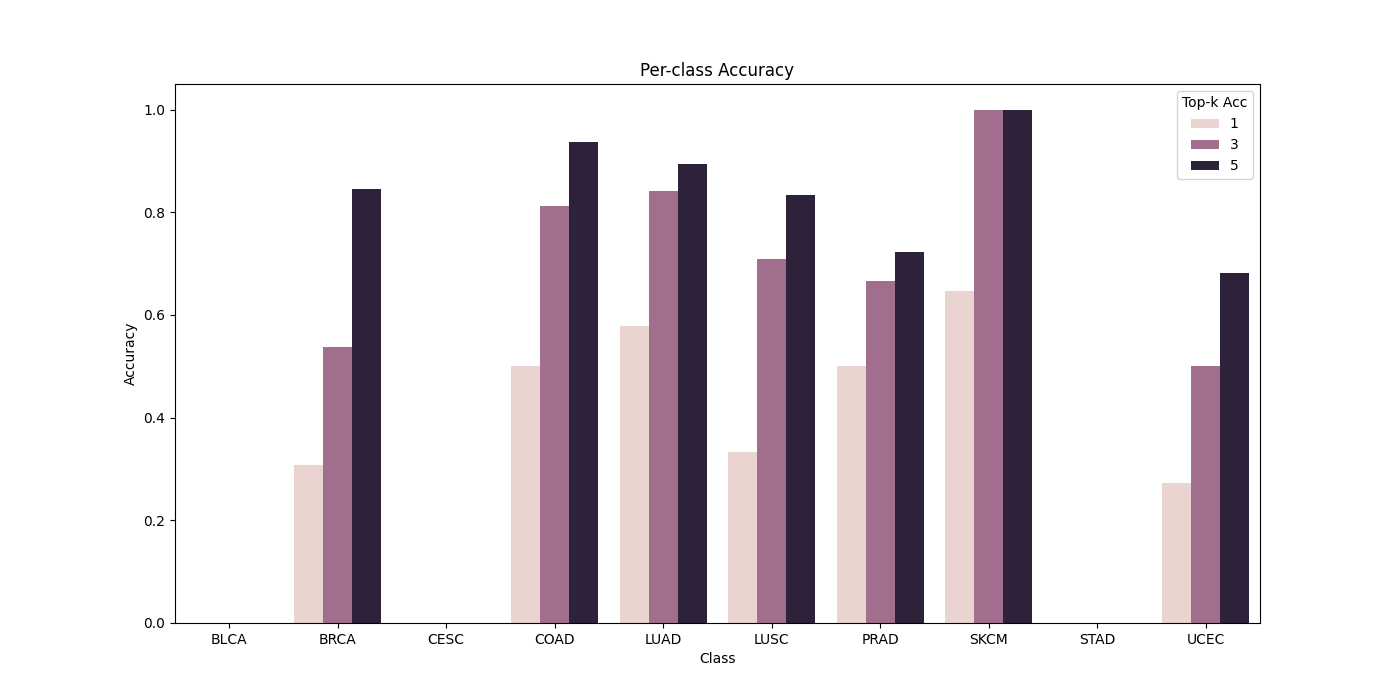
\includegraphics[width=1\linewidth]{images/class_accuracy.png}
    \caption{A figure showing per-class accuracy performance of LeakyPanCancerClassifier model on the external dataset. The model was trained on TCGA data and evaluated using top-1, top-3, and top-5 accuracy metrics. BLCA, CESC, and STAD classes showed zero accuracy as they were absent from the external dataset. The metrics were lower compared to the 5-fold cross-validation results.}
    \label{fig:class-acc-ext}
\end{figure}

\begin{figure}[h!]
    \centering
    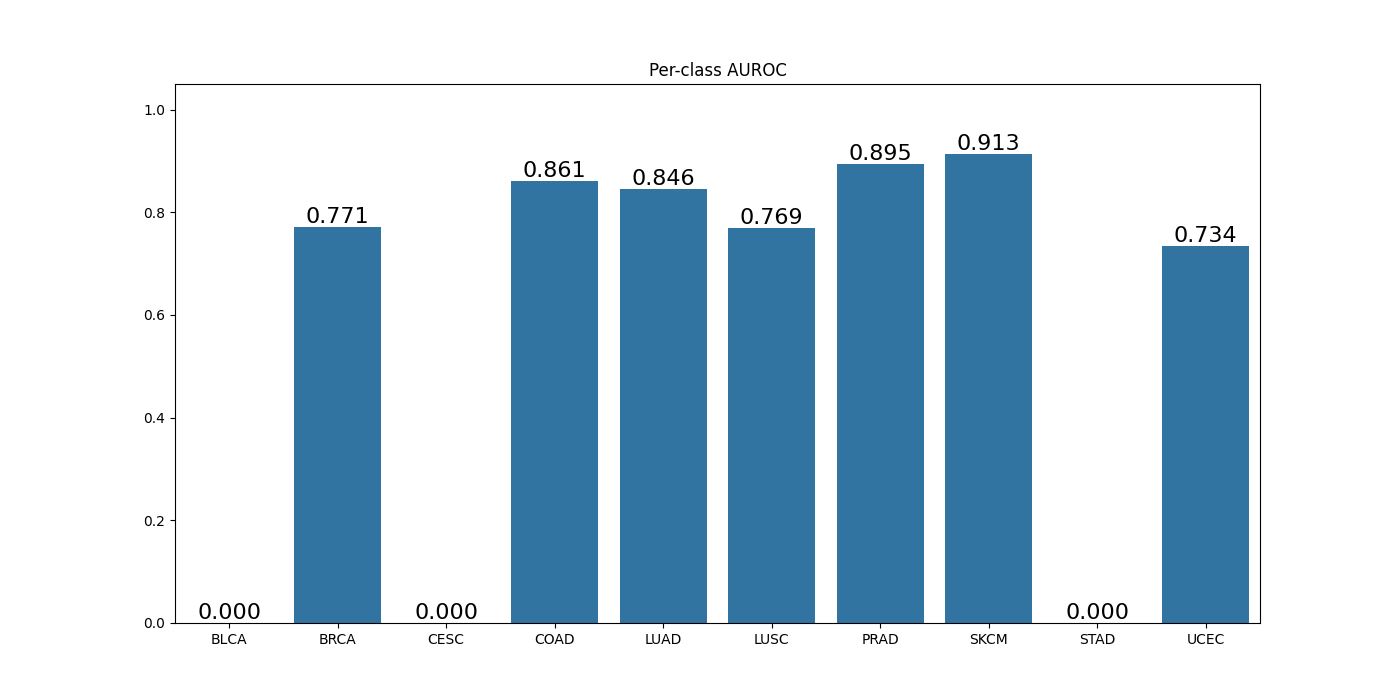
\includegraphics[width=1\linewidth]{images/class_auroc.png}
    \caption{Per-class AUROCs of LeakyPanCancerClassifier model on the external dataset. AUROCs for BLCA, CESC, and STAD were zero due to their absence from the dataset. There was a drop in AUROC when compared to the 5-fold cross-validation results on the TCGA dataset.}
    \label{fig:class-auroc-ext}
\end{figure}

On the external dataset, the model achieved top-1 accuracy of 0.442, top-3 accuracy of 0.721, and top-5 accuracy of 0.798. There was a significant drop from the previous cross-validation results of 0.689, 0.899, and 0.962, respectively. 

We hypothesised several factors that can contribute to the lowered performance:
\begin{itemize}
    \item The external testing set was not as \emph{curated} as the TCGA dataset used to train and perform cross-validation. For example, there was no minimum number of tiles criterion for inclusion for the external set. This was a deliberate choice to evaluate classifier performance in a less controlled environment. For details on the inclusion criteria of the TCGA dataset, readers can refer to the HPL paper.
    \item There might be differences in how the histology slides were prepared for each source, which could adversely affect model performance. The model was trained exclusively on TCGA data, so it was optimised for the specific preparation standards employed by TCGA.
\end{itemize}

\section{Out-of-Distribution Test Results} \label{sec:ood-results}

Out-of-Distribution(OoD) testing is conducted to investigate the model's response to data that substantially deviates from the training set. Data from TCGA, CMB, and CPTAC all contained cancer tissue. This section examines the model's behaviour on WSIs that do not contain cancerous areas at all. GTEx project, which only contains WSIs of normal tissue, served as the data source for this OoD testing.

Cancer WSIs from the TCGA contain portions of normal tissue mixed with malignant regions. For example, a lung adenocarcinoma (LUAD) WSI typically includes areas that contain malignant tissues alongside relatively normal structures such as lung parenchyma, vessels, and connective tissues. The WSI vector is a representation of the entire WSI, so it can be said that the model sees both the malignant parts and the normal parts of the WSI. In some cases, malignant regions can look similar between different tissues, with differentiation possible only through observing the surrounding tissues. Therefore it is sensible for a classifier model to see both portions.

The TCGA training set was limited to primary tumours. Being a primary tumour means that the malignancy is not metastatic, so the lung cancer slides --- LUAD and LUSC --- are always lung tissue slides. Therefore, we expected the model to perform decently well with this dataset.

Normal tissue sources from GTEx were mapped to corresponding cancer types. For example, a stomach WSI from GTEx was mapped to stomach adenocarcinoma (STAD) for the classifier. The sole exception to this was lung tissue, since the classifier differentiates between lung adenocarcinoma (LUAD) and lung squamous cell carcinoma (LUSC), which are both lung malignancies. All normal lung WSIs from GTEx were mapped to LUAD. The number of samples and the tissue sources, along with their mappings, can be seen in Table \ref{tab:gtex}. In total, the GTEx dataset comprised 188 normal WSIs.

\begin{table}[b]
\centering
\caption{A table showing class distribution of the GTEx dataset (188 WSIs total) along with the tissue source mappings to the classifier's classes. All lung samples were mapped to LUAD, which is index 4, so LUSC (index 5) is omitted from the table.}
\label{tab:gtex}
\rowcolors{2}{}{gray!3}
\begin{tabular}{@{}llll@{}}
\textbf{Index} & \textbf{Tissue (GTEx)}                                                                                    & \textbf{Class} & \textbf{\# of Samples} \\ \midrule
0              & Bladder                                                                                                   & BLCA           & 17                     \\
1              & Breast                                                                                                    & BRCA           & 17                     \\
2              & Ectocervix                                                                                                & CESC           & 16                     \\
3              & Transverse Colon, Sigmoid Colon                                 & COAD           & 18                     \\
4              & Lung                                                                                                      & LUAD           & 33                     \\
6              & Prostate                                                                                                  & PRAD           & 20                     \\
7              & \begin{tabular}[c]{@{}l@{}}Non sun-exposed Skin (Suprapubic),\\ Sun-exposed Skin (Lower Leg)\end{tabular} & SKCM           & 23                     \\
8              & Stomach                                                                                                   & STAD           & 28                     \\
9              & Uterus                                                                                                    & UCEC           & 16                    
\end{tabular}
\end{table}

As with the external dataset, the discussed results were from the LeakyPanCancerClassifier model. The model was trained with the TCGA dataset, with the HPL models frozen since the start, and the classifier model frozen from cross-validation. With the mappings, the model achieved top-1 accuracy of 0.362, top-3 accuracy of 0.770, and top-5 accuracy of 0.891. Class-specific accuracies are illustrated in Figure \ref{fig:class-acc-gtex}. These accuracy numbers are comparable to those obtained on the external dataset.

\begin{figure}[h]
    \centering
    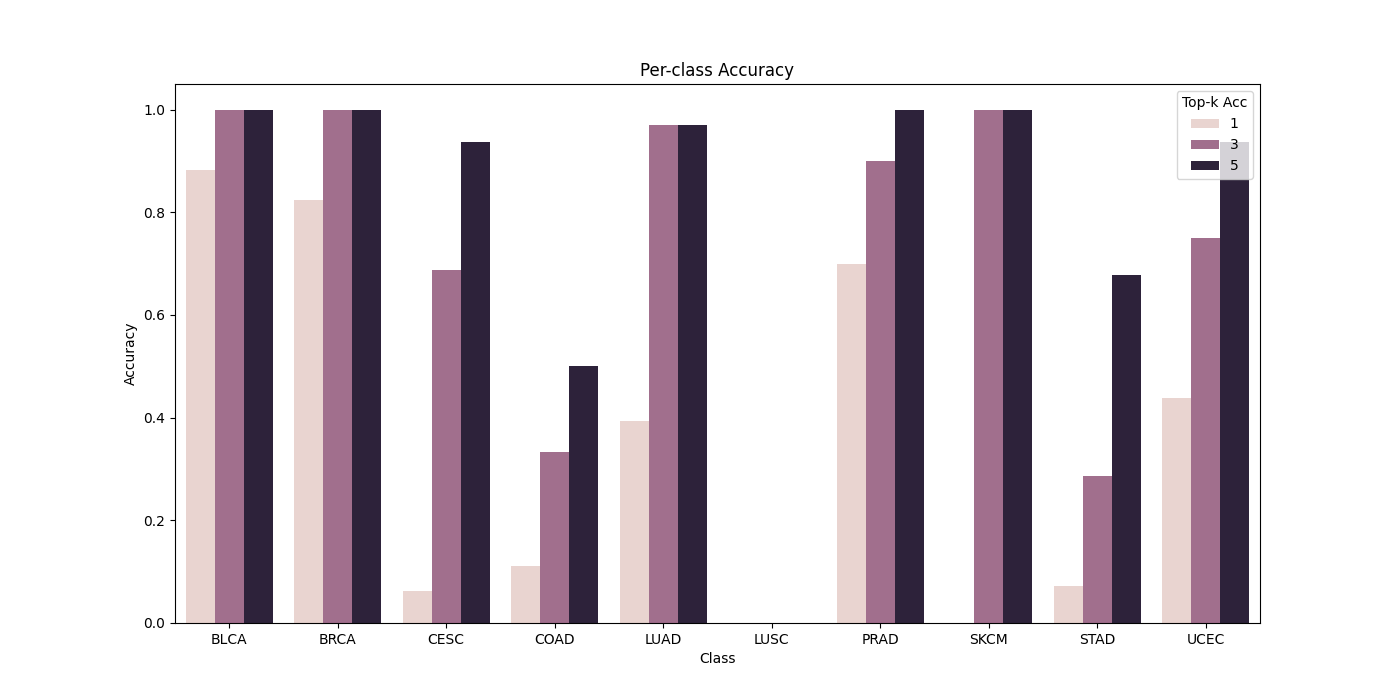
\includegraphics[width=1\linewidth]{images/gtexacc.png}
    \caption{Per-class top-k accuracies (k = 1, 3, 5) for the LeakyPanCancerClassifier model on the GTEx dataset. The top-k accuracies for LUSC were zero due to the mapping of lung tissues to LUAD. The performances were comparable to the results on the external dataset, despite the slight handicap as a result of mapping every lung sample to LUAD.}
    \label{fig:class-acc-gtex}
\end{figure}

The accuracy reported here might have been artificially lowered because of the mix-up between the two lung cancer types, as only lung tissue slides classified as LUAD were considered correct. However, examination of the modified confusion matrix in Figure \ref{fig:conf-mat-gtex} revealed that only few samples were classified as LUSC.

\begin{figure}[h]
    \centering
    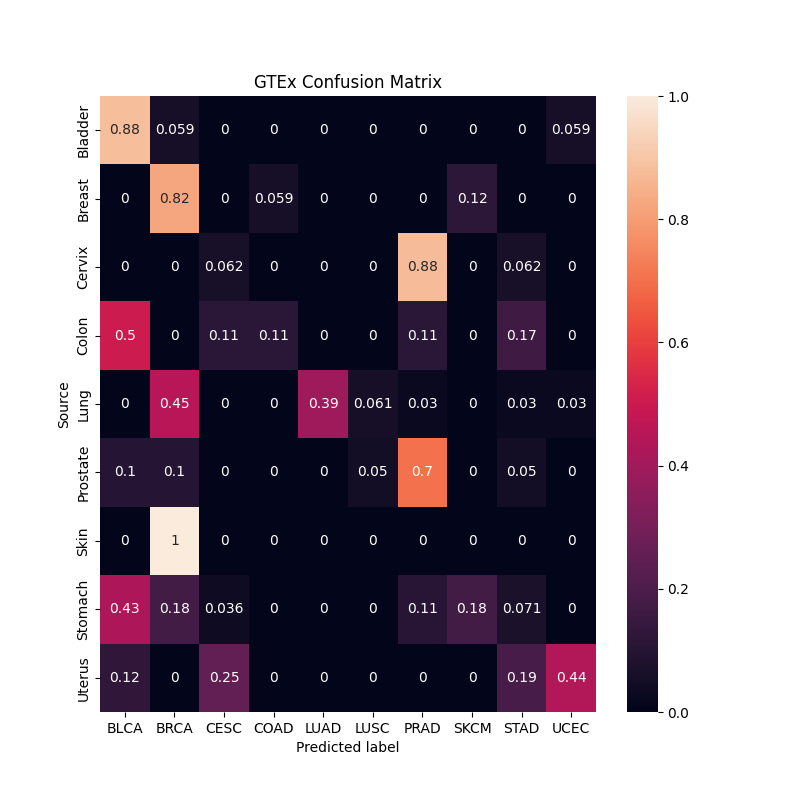
\includegraphics[width=0.8\linewidth]{images/confusion_matrix.png}
    \caption{Modified confusion matrix from evaluating the LeakyPanCancerClassifier model on the GTEx dataset. The rows correspond to tissue sources from GTEx while the columns correspond to predictions by the model. There are fewer rows than columns due to the redundant LUSC in the columns. There were only a few samples that get classified as LUSC by the model. A majority of cervix tissue samples were misclassified as PRAD (prostate), and skin samples as BRCA (breast).}
    \label{fig:conf-mat-gtex}
\end{figure}

The model exhibited unexpected misclassification patterns: cervix tissue samples were consistently predicted to be PRAD, \emph{prostate} adenocarcinoma, and all skin samples were classified by the model as BRCA, \emph{breast} invasive carcinoma. These unanticipated prediction patterns warranted further investigation of the SHAP values. The SHAP values for BRCA and PRAD predictions are presented in Figures \ref{fig:shap-brca} and \ref{fig:shap-prad} respectively.

\begin{figure}[h]
    \centering
    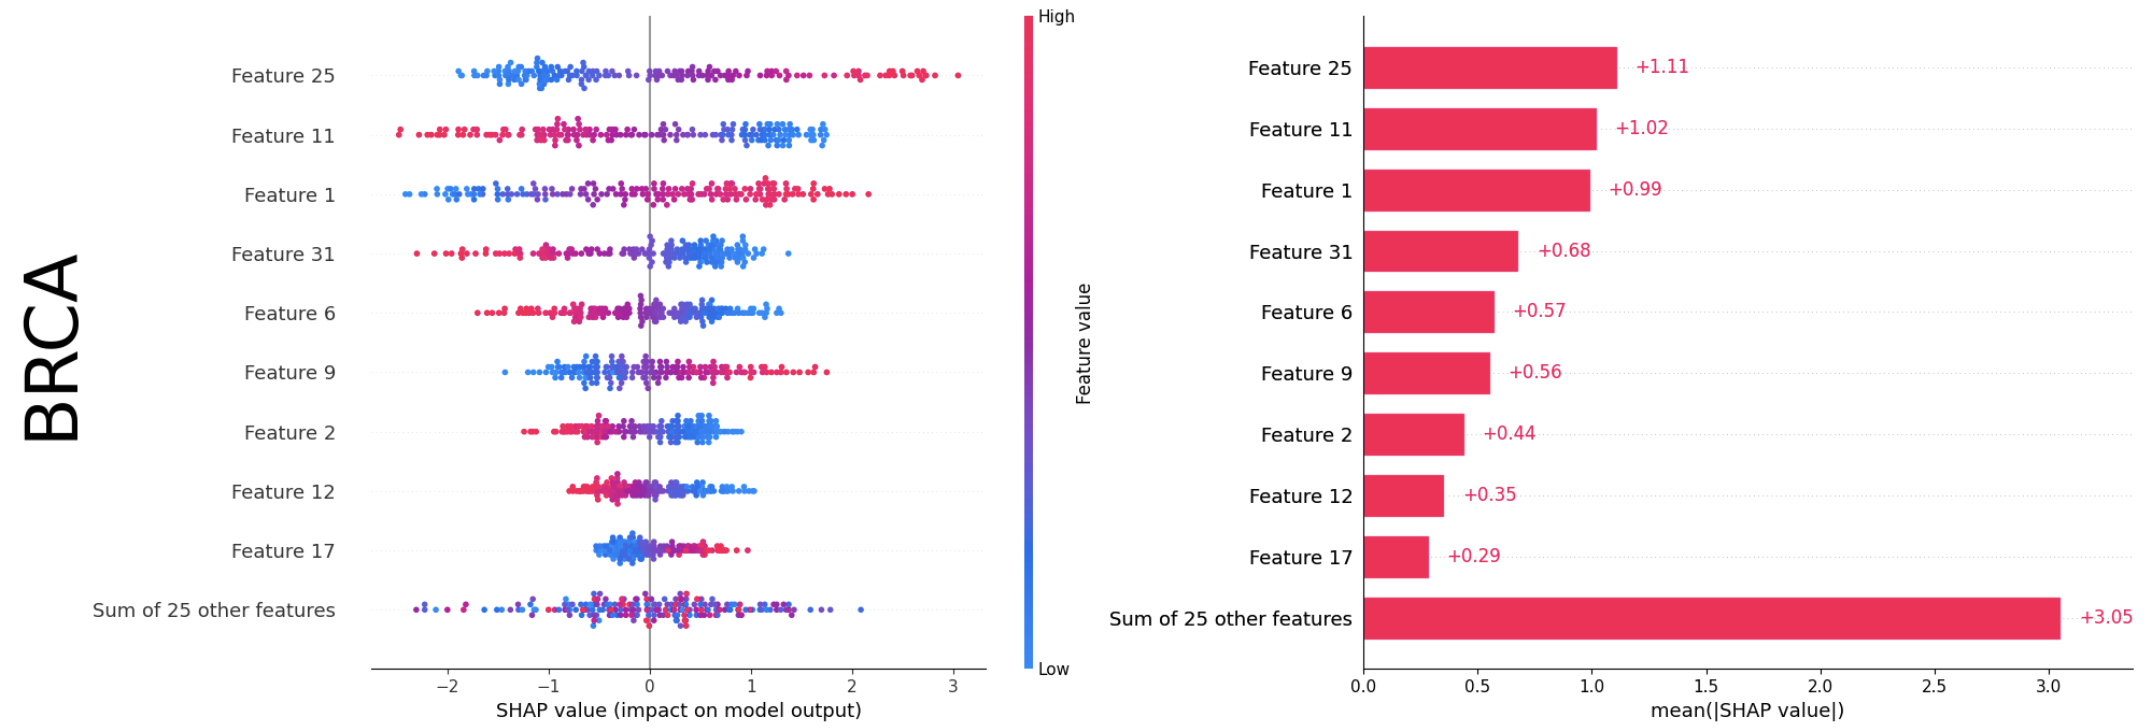
\includegraphics[width=1\linewidth]{images/brca-shap.png}
    \caption{Beeline plot of SHAP values (left) and bar chart of average of absolute SHAP values (right) for BRCA prediction by the LeakyPanCancerClassifier model. The SHAP values were calculated from the GTEx dataset. High values of feature 25 and feature 1 contributed significantly to positive BRCA predictions. Low value of feature 11 also contributed strongly to BRCA predictions, but this represented the absence of HPC 11, which was harder to investigate.}
    \label{fig:shap-brca}
\end{figure}

\begin{figure}[h]
    \centering
    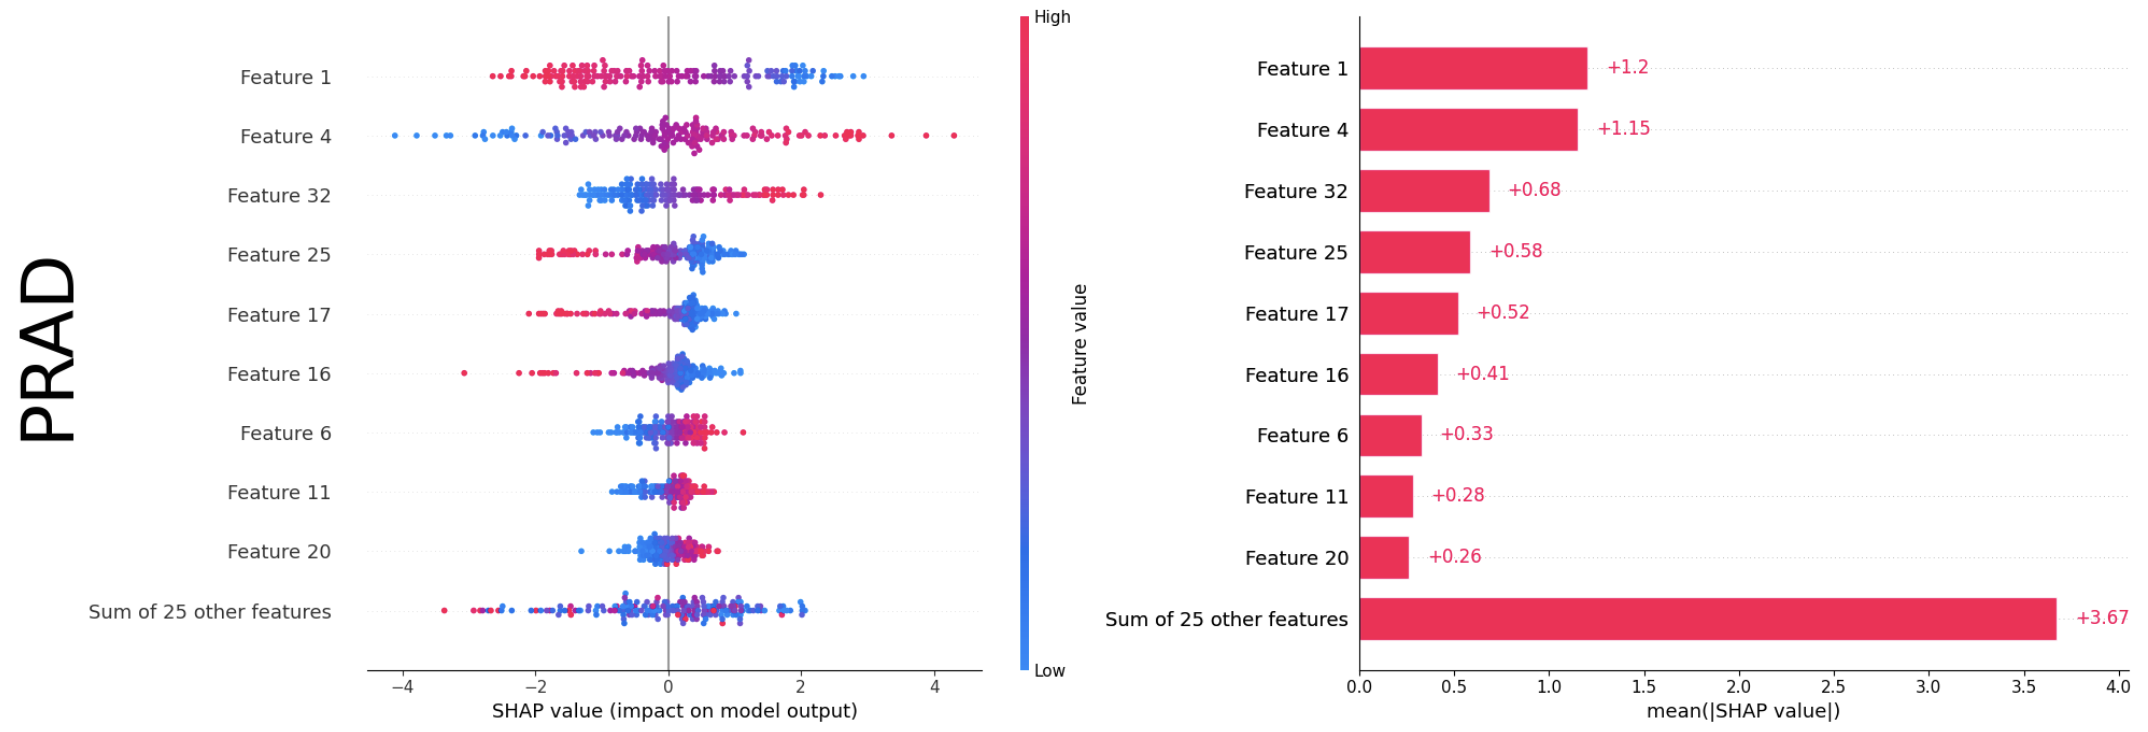
\includegraphics[width=1\linewidth]{images/prad-shap.png}
    \caption{Beeline plot of SHAP values (left) and bar chart of average of absolute SHAP values (right) for PRAD prediction by the LeakyPanCancerClassifier model. The SHAP values were calculated from the GTEx dataset. High value of feature 4 contributed significantly to positive PRAD predictions. Low value of feature 1 contributed the largest to PRAD predictions.}
    \label{fig:shap-prad}
\end{figure}

Analysis of SHAP values revealed that high values of features 25 and 1 supported BRCA classification by the classifier, while feature 4 exhibited a similar influence on PRAD predictions. Since each feature in the WSI vector could be traced back to a particular HPC clustered by the HPL methodology, these clusters could be directly examined. HPCs 25 and 1 from breast and skin tissues were compared, as well as HPC 4 from prostate and cervix tissues. Figures \ref{fig:hpc25} and \ref{fig:hpc1} present the images of tiles from HPCs 25 and 1 from breast and skin tissues. HPC 25 tile images from prostate and cervix tissues are shown in Figure \ref{fig:hpc4}.

Certain histological characteristics are shared among multiple tissues. For instance, adipocytes are present in the hypodermis layer of skin tissue and in breast tissue alongside mammary glands. Therefore, it was reasonable that HPCs that correspond to such shared characteristics, such as HPC 1, contribute to positive predictions for both skin and breast classes.

There are structures that may be similar in both structure and appearance, but constitute different things depending on the tissue context. HPC 25 captured dense connective tissue areas in both skin and breast samples. However, within the skin tissue context, the net-like appearance specifically indicated the reticular dermis layer.

Additionally, there are structures with appearances that may resemble one another but are vastly different structures. Examining HPC 4 tiles from cervix WSIs consistently revealed tiles that contained vessels. Doing the same with prostate WSIs predominantly captured prostatic glands instead. 

\section{Discussion} \label{sec:discuss-classifier}
 Cross-validation results with the TCGA dataset suggested that the models could learn patterns in the WSI vectors, given by high AUROC, but the predictions fell short of being outright correct most of the time. The results imply that there are limitations to using WSI vectors as described as representations of WSIs for cancer classification purposes.

OoD testing with the GTEx dataset showed that HPCs represented visually similar tiles. However, tiles that look alike are not necessarily the same tissue structure. Examining tiles with the same HPC from different tissues often revealed different structures sharing certain visual characteristics. Within the same tissue context, HPCs demonstrated greater purity and coherence. For example, as seen in Figure \ref{fig:prostate4}, the tiles clustered as HPC 4 consistently had the appearance of prostatic glands. This suggests that the approach of clustering visually similar tiles is more effective when confined to a particular tissue context.

HPC purity and coherence were higher within the same tissue type, but there was still some noise in the clusters under the same tissue context. We believed that this noise resulted from the clustering process being too coarse. With the frozen clustering model, there were only 34 HPCs, representing all tissue morphologies of 10 cancer types, from 9 anatomical locations. In this case, the Leiden resolution, which determines how coarse or fine the clustering process is, was likely too low for the needs of this application. This exemplifies the importance of hyperparameters of HPL methodology on the success of downstream applications.

For the purpose of determining cancer types with WSI representations, the model processed both malignant and non-malignant tissue regions, with the latter providing tissue context. We suggest that when the training data consists exclusively of primary tumour WSIs, the model may inadvertently learn to recognise patterns in the surrounding normal tissue rather than patterns of malignant areas. This is supported by roughly equal performance metrics observed between the external dataset and the GTEx dataset used for OoD testing. This observation suggested that the model would perform poorly when classifying metastatic cancer. Incorporating metastases into the training data is crucial for teaching the model to be less reliant on the tissue context.

Finally, significant differences between the training data and real-world applications may cause the model to perform considerably worse. Histological slide preparation may differ between data projects and sources. This likely contributed to the performance disparity between the TCGA dataset in cross-validation and the external dataset. A diverse training dataset from multiple sources and distributions may increase the robustness of the model.

\begin{figure}[h]
    \centering
    \begin{subfigure}[b]{\textwidth}
        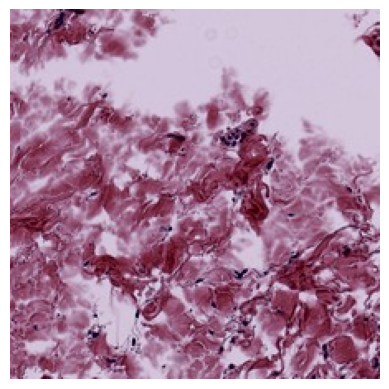
\includegraphics[width=0.24\textwidth]{images/skin25_1.png}
        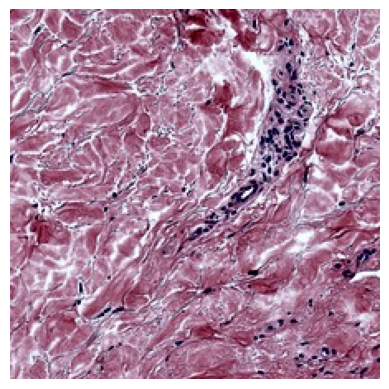
\includegraphics[width=0.24\textwidth]{images/skin25_2.png}
        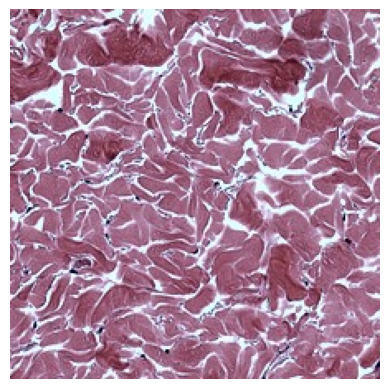
\includegraphics[width=0.24\textwidth]{images/skin25_3.png}
        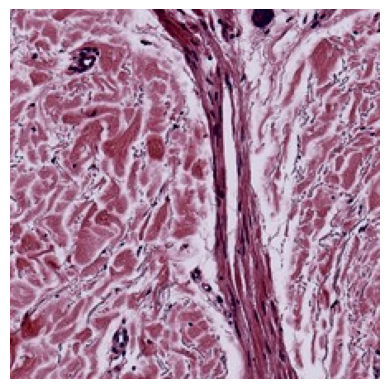
\includegraphics[width=0.24\textwidth]{images/skin25_4.png}
        \caption{Skin(25): GTEX-15SHV-2026, GTEX-11GSO-2426, GTEX-11ZUS-0626, GTEX-132AR-0126}
        \label{fig:skin25}
    \end{subfigure}
    \begin{subfigure}[b]{\textwidth}
        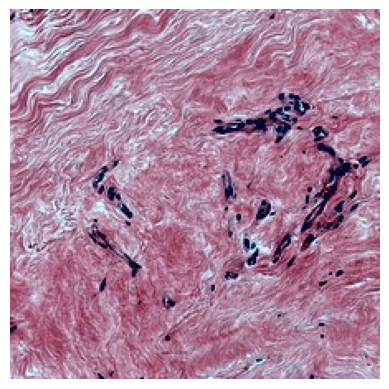
\includegraphics[width=0.24\textwidth]{images/breast25_1.png}
        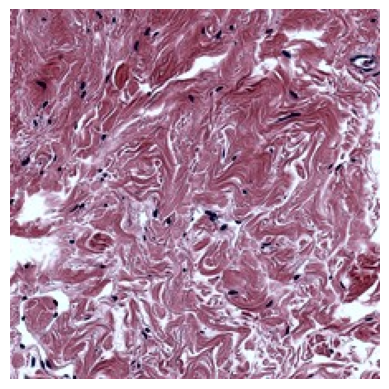
\includegraphics[width=0.24\textwidth]{images/breast25_2.png}
        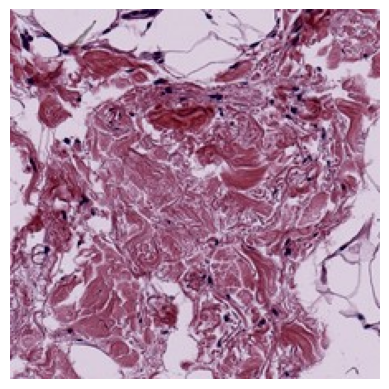
\includegraphics[width=0.24\textwidth]{images/breast25_3.png}
        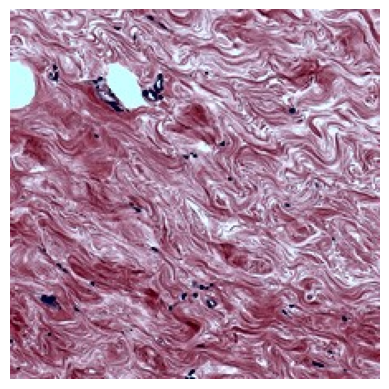
\includegraphics[width=0.24\textwidth]{images/breast25_4.png}
        \caption{Breast(25): GTEX-11GS4-2126, GTEX-111VG-1226, GTEX-111CU-1626, GTEX-13OVJ-2226}
        \label{fig:breast25}
    \end{subfigure}
    \caption{Tile images of HPC 25 from GTEx dataset. \subref{fig:skin25} contains tile images from skin tissue, and \subref{fig:breast25} from breast tissue. HPC 25 captured patch of connective tissue. While for breast the tile images seemed to contain generic fibrous areas, for skin they captured a specific appearance of the reticular dermis. WSI's sample IDs from which the tile images were taken are noted below each row, left to right.
    }\label{fig:hpc25}
\end{figure}

\begin{figure}[t]
    \centering
    \begin{subfigure}[b]{\textwidth}
        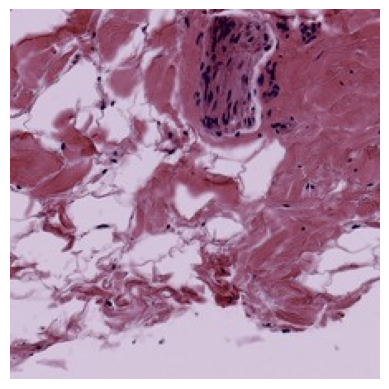
\includegraphics[width=0.24\textwidth]{images/skin1_1.png}
        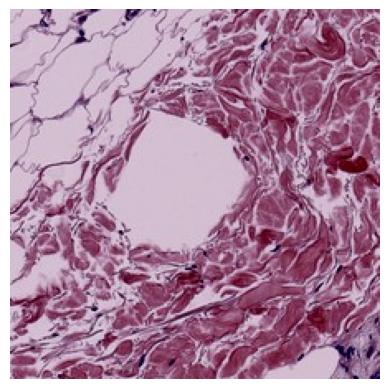
\includegraphics[width=0.24\textwidth]{images/skin1_2.png}
        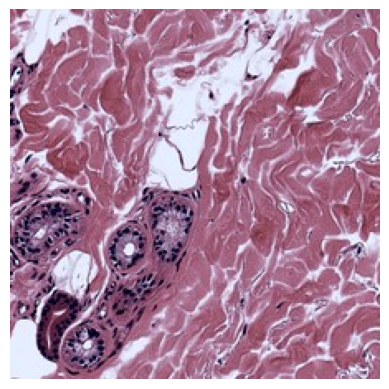
\includegraphics[width=0.24\textwidth]{images/skin1_3.png}
        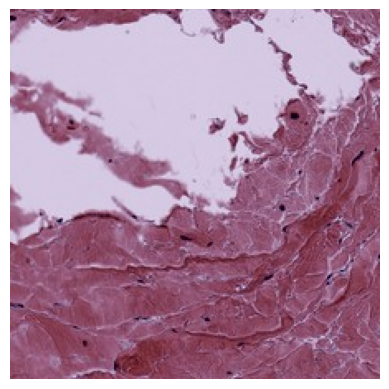
\includegraphics[width=0.24\textwidth]{images/skin1_4.png}
        \caption{Skin(1): GTEX-15SHV-2026, GTEX-11GSO-2426, GTEX-11ZUS-0626, GTEX-145LU-0126}
        \label{fig:skin1}
    \end{subfigure}
    \begin{subfigure}[b]{\textwidth}
        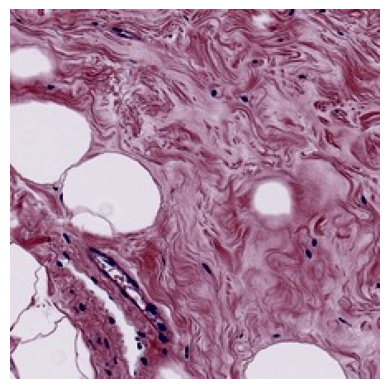
\includegraphics[width=0.24\textwidth]{images/breast1_1.png}
        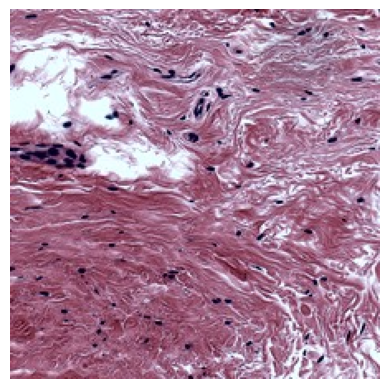
\includegraphics[width=0.24\textwidth]{images/breast1_2.png}
        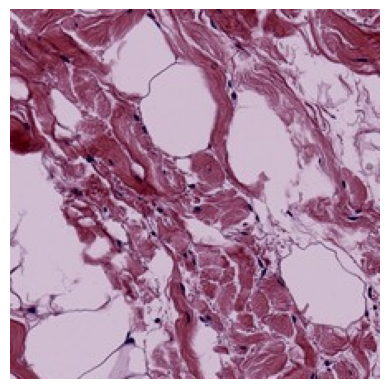
\includegraphics[width=0.24\textwidth]{images/breast1_3.png}
        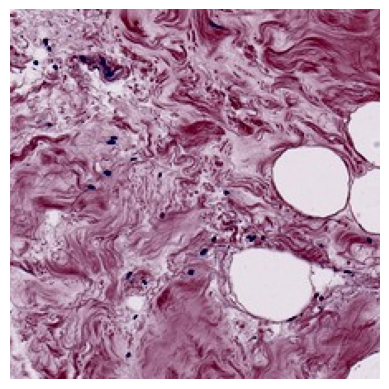
\includegraphics[width=0.24\textwidth]{images/breast1_4.png}
        \caption{Breast(1): GTEX-11GS4-2126, GTEX-111VG-1226, GTEX-111CU-1626, GTEX-13OVJ-2226}
        \label{fig:breast1}
    \end{subfigure}
    \caption{Tile images of HPC 1 from the GTEx dataset. \subref{fig:skin1} contains tile images from skin tissue and \subref{fig:breast1} from breast tissue. HPC 1 seemed to be capturing high exposure area (e.g., adipose cells, or artifacts) surrounded by patches of connective tissues. 
    }\label{fig:hpc1}
\end{figure}

\begin{figure}[h]
    \centering
    \begin{subfigure}[b]{\textwidth}
        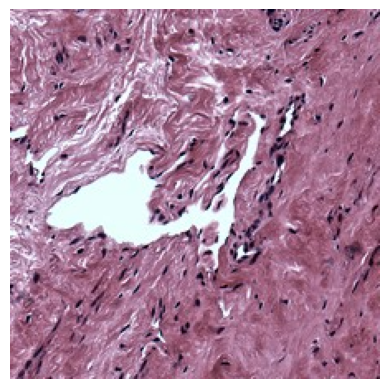
\includegraphics[width=0.24\textwidth]{images/cervix4_1.png}
        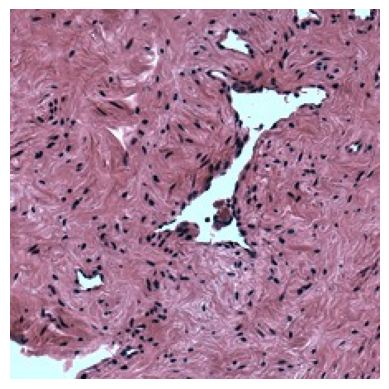
\includegraphics[width=0.24\textwidth]{images/cervix4_2.png}
        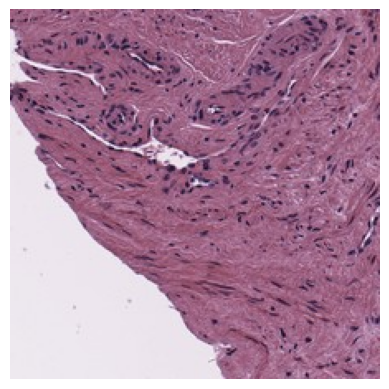
\includegraphics[width=0.24\textwidth]{images/cervix4_3.png}
        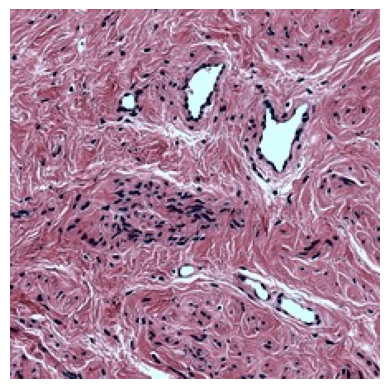
\includegraphics[width=0.24\textwidth]{images/cervix4_4.png}
        \caption{Cervix(4): GTEX-T5JW-0726, GTEX-U3ZN-1526, GTEX-POMQ-1526,GTEX-PWCY-1626}
        \label{fig:cervix4}
    \end{subfigure}
    \begin{subfigure}[b]{\textwidth}
        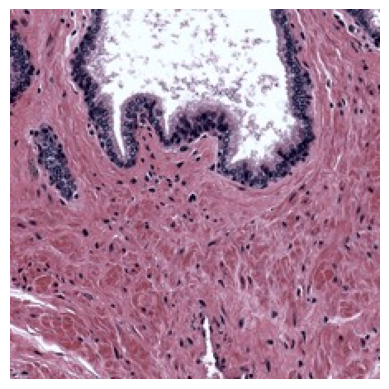
\includegraphics[width=0.24\textwidth]{images/prostate4_1.png}
        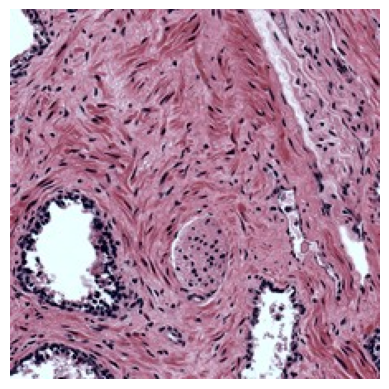
\includegraphics[width=0.24\textwidth]{images/prostate4_2.png}
        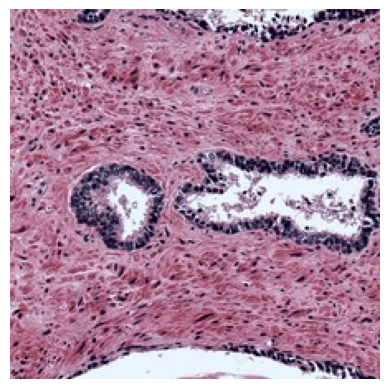
\includegraphics[width=0.24\textwidth]{images/prostate4_3.png}
        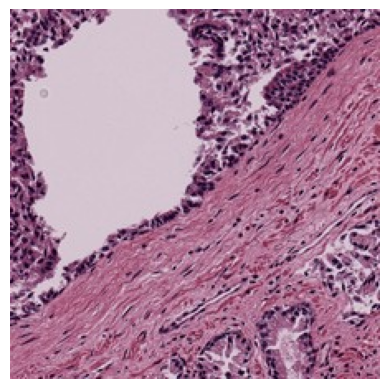
\includegraphics[width=0.24\textwidth]{images/prostate4_4.png}
        \caption{Prostate(4): GTEX-1399R-052, GTEX-13RTJ-2126, GTEX-13RTJ-2126, GTEX-111FC-2026}
        \label{fig:prostate4}
    \end{subfigure}
    \caption{Tile images of HPC 4 from the GTEx dataset. \subref{fig:cervix4} contains tile images from cervix tissue, and \subref{fig:prostate4} are from prostate tissue. Luminal structures were captured by HPC 4. However, this corresponded to different structures depending on the tissue. For cervix, it captured vessels, while for prostate, tiles containing prostatic glands were clustered into HPC 4 instead.
    }\label{fig:hpc4}
\end{figure}

%==================================================================================================================================
\chapter{Generating Captions for Individual Lung Cancer Tile Images} \label{sec:caption}

This chapter addresses the second research question: how to create a model that can automatically generate descriptive captions for individual cancer tile images. To achieve this, we introduced a new workflow for generating tile-level annotations by leveraging the HPL methodology. The HPC annotations were paired with the tile images in each HPC to create the training dataset for the tile image captioning model.

A detailed explanation of how the tile-level captions were generated for the dataset is provided in Section \ref{sec:data-workflow}. The architecture of the model is described in Section \ref{sec:caption-model}, while the training process is outlined in Section \ref{sec:caption-training}. The results are shown and discussed in Sections \ref{sec:caption-results} and \ref{sec:caption-discussion}, respectively.

\section{Data Workflow} \label{sec:data-workflow}
As highlighted in Section \ref{sec:WSI_anatomy}, one of the main challenges of applying machine learning to medical images, particularly histopathology images, is the scarcity of high-quality annotations. This is especially true for tile-level labels. HPL methodology (Section \ref{sec:HPL}) offers a solution by clustering visually similar tissue tiles into clusters called HPCs. This clustering approach can serve as an efficient tool for facilitating tile-level annotation for expert pathologists.

Rather than annotating each tile individually, which is very time-consuming, or annotating regions of the slide, which may lack specificity, HPL methodology allows annotating an entire cluster of tile images at once. Each HPC contains visually similar tiles, which typically correspond to the same histological landscape. The annotations made at the cluster level can then be propagated back to all member tile images of that cluster. This gives tile-annotation pairings which can serve as training data for supervised learning.

We applied the workflow described to train an image captioning model by using the tile-annotation pairings created through the aforementioned method. The workflow is illustrated in Figure \ref{fig:data-workflow}. 

\begin{figure}[h]
    \centering
    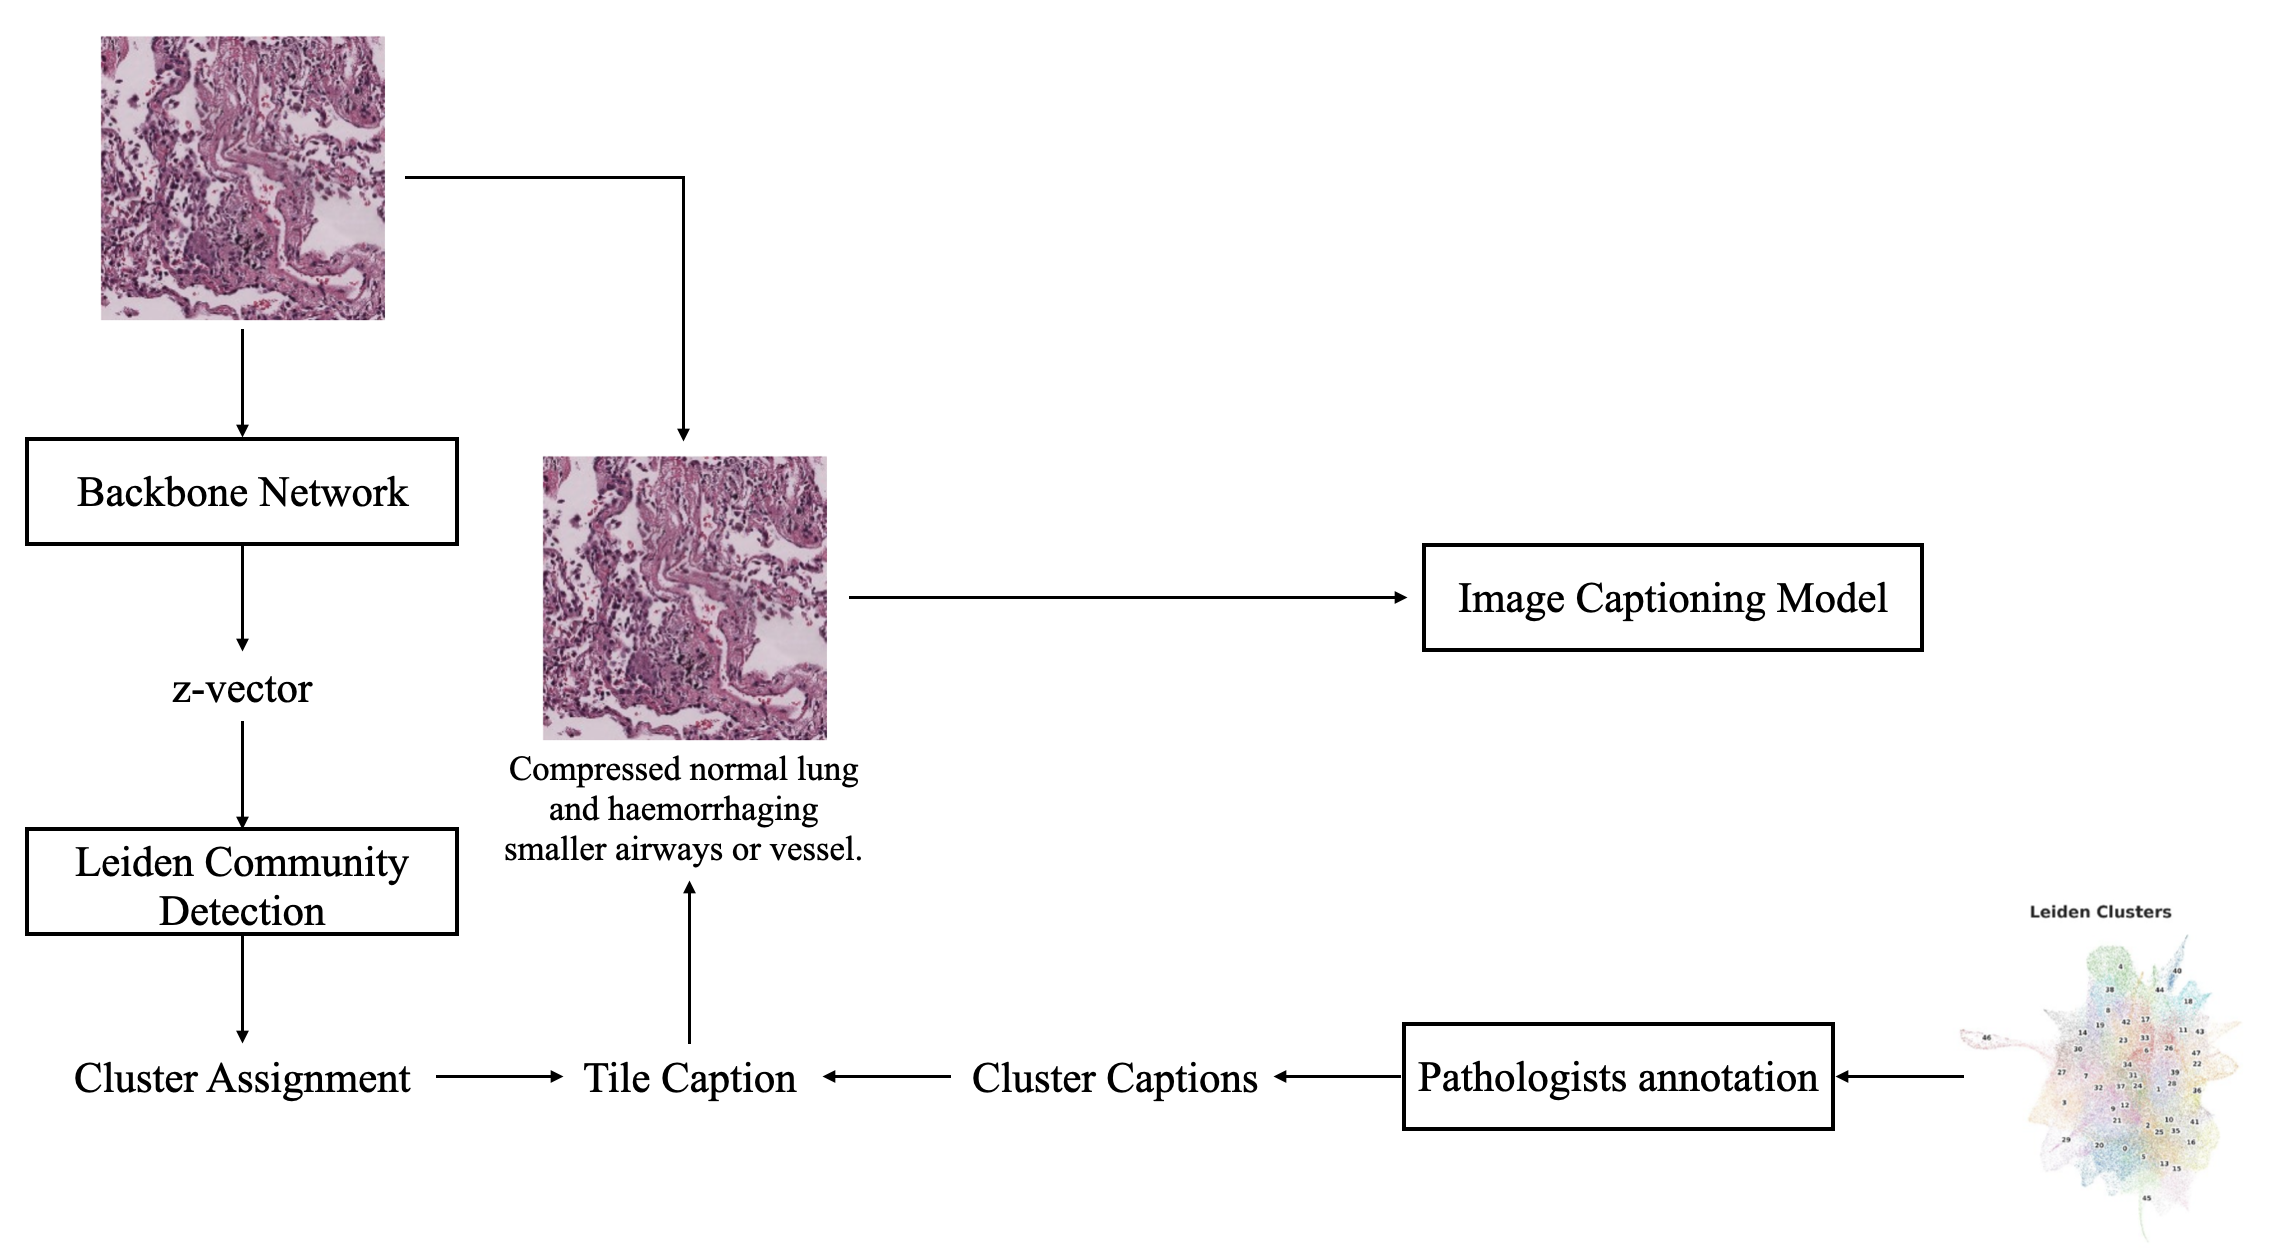
\includegraphics[width=1\linewidth]{images/workflow_diagram.png}
    \caption{Workflow diagram of generating a tile-annotation pairings for the purpose of supervised learning. The dataset is clustered using HPL methodology, and each HPC is annotated by expert pathologists. The cluster caption is put on the members of that cluster, creating tile-annotation pairings suitable for supervised learning. This tile is from slide sample TCGA-97-8179-01Z-00-DX1 sourced from the TCGA dataset. The visualisation of Leiden clusters (bottom right) is adapted from the HPL paper \citep{ClaudioQuiros2024}.}
    \label{fig:data-workflow}
\end{figure}

\section{Models} \label{sec:caption-model}

The tile image captioning model employs a CNN-RNN architecture. The CNN encodes tile images into feature vectors that capture visual information of the tiles. The RNN functions as a text decoder, which translates these feature vectors into natural text captions that describe the histological features present in the tile images.

We used the frozen backbone model from HPL methodology as the CNN image feature extractor. The HPL backbone model produces two distinct representations: a dense z-vector of size 128 ($\boldsymbol{z} \in \mathbb{R}^{128}$), and a sparse h-vector of size 1024 ($\boldsymbol{h} \in \mathbb{R}^{1024}$). Within the backbone model, the image is passed through a series of ResNet layers and traditional convolutional layers first, and the output from this set is flattened, creating the h-vector. Subsequently, the h-vector is passed through a series of fully connected layers, interspersed with batch normalisation and ReLU activation functions to produce the z-vector.

The vocabulary was derived from the collection of cluster annotations, which covered all possible captions in the dataset. We used the tokeniser from spaCy\footnote{https://spacy.io} library for splitting a sentence into a series of tokens. Three special tokens were added to the vocabulary:
\begin{itemize}
    \item \verb|<SOS>| (start-of-sequence) token added before any sentences
    \item \verb|<EOS>| (end-of-sequence) token appended to the end of all sentences
    \item \verb|<PAD>| (padding) token used for equalising sequence lengths when grouped into batches
\end{itemize}
All tokens besides the special tokens were converted to all lowercase characters. The final vocabulary size was 130.

% Firstly, the text is split into a series of tokens. This paper uses the English language tokeniser implemented in the spaCy\footnote{https://spacy.io} library. For the purpose of caption generation, two special tokens are appended to the list of tokens. \verb|<SOS>| (start-of-sequence) token is appended to the beginning, and \verb|<EOS>| (end-of-sequence) token is appended to the end. For data batching purposes, \verb|<PAD>| (padding) token may be appended at the end, after end-of-sequence token, to allow stacking of multiple embedding tensors. Padding tokens are ignored during training. All tokens, except special tokens, are converted to lowercase.

% Afterwards, the list of tokens is transformed to a vector of indices via a look up table, called the \emph{vocabulary}. The vocabulary is built by looking through the entire corpus of caption data. Each unique token in the corpus that appears above a certain number of times (threshold), will be allocated a unique index. The vocabulary can perform string to index (stoi) transformation, or index to string (itos).

% The vector of indices can be transformed into a tensor of one-hot vectors, each referring to one word token. The one-hot vector is a sparse vector which has the value of 0 in all elements except the specified index, for which the value is 1. The length of the one-hot vector is equal to the length of the vocabulary.

% Lastly, the one-hot vectors are transformed into word embeddings by using a look-up table in the form of a tensor. The dot product of one-hot vectors and the embedding tensor is calculated. The output is a tensor of word embeddings with a specific length. Unlike one-hot vectors, embeddings are dense, and are more efficient for machine learning tasks.

For the text generation component, the model uses an LSTM network, a version of RNN. The output from the frozen image feature encoder is first passed through a non-frozen fully connected layer. This trainable layer enables the model to learn task-specific qualities relevant to the captioning objective. The output from the layer is called the image embedding. This embedding is then fed into the LSTM network. At each timestep, the LSTM's output is passed to a linear layer that maps it to the logit values corresponding to the probability distribution over the next token prediction. The model outputs a vector with the dimension matching the vocabulary size, with each element representing the raw logit for each token in the vocabulary. The complete architecture of the model is sketched in Figure \ref{fig:lstm-cap}.

\begin{figure}[h!]
    \centering
    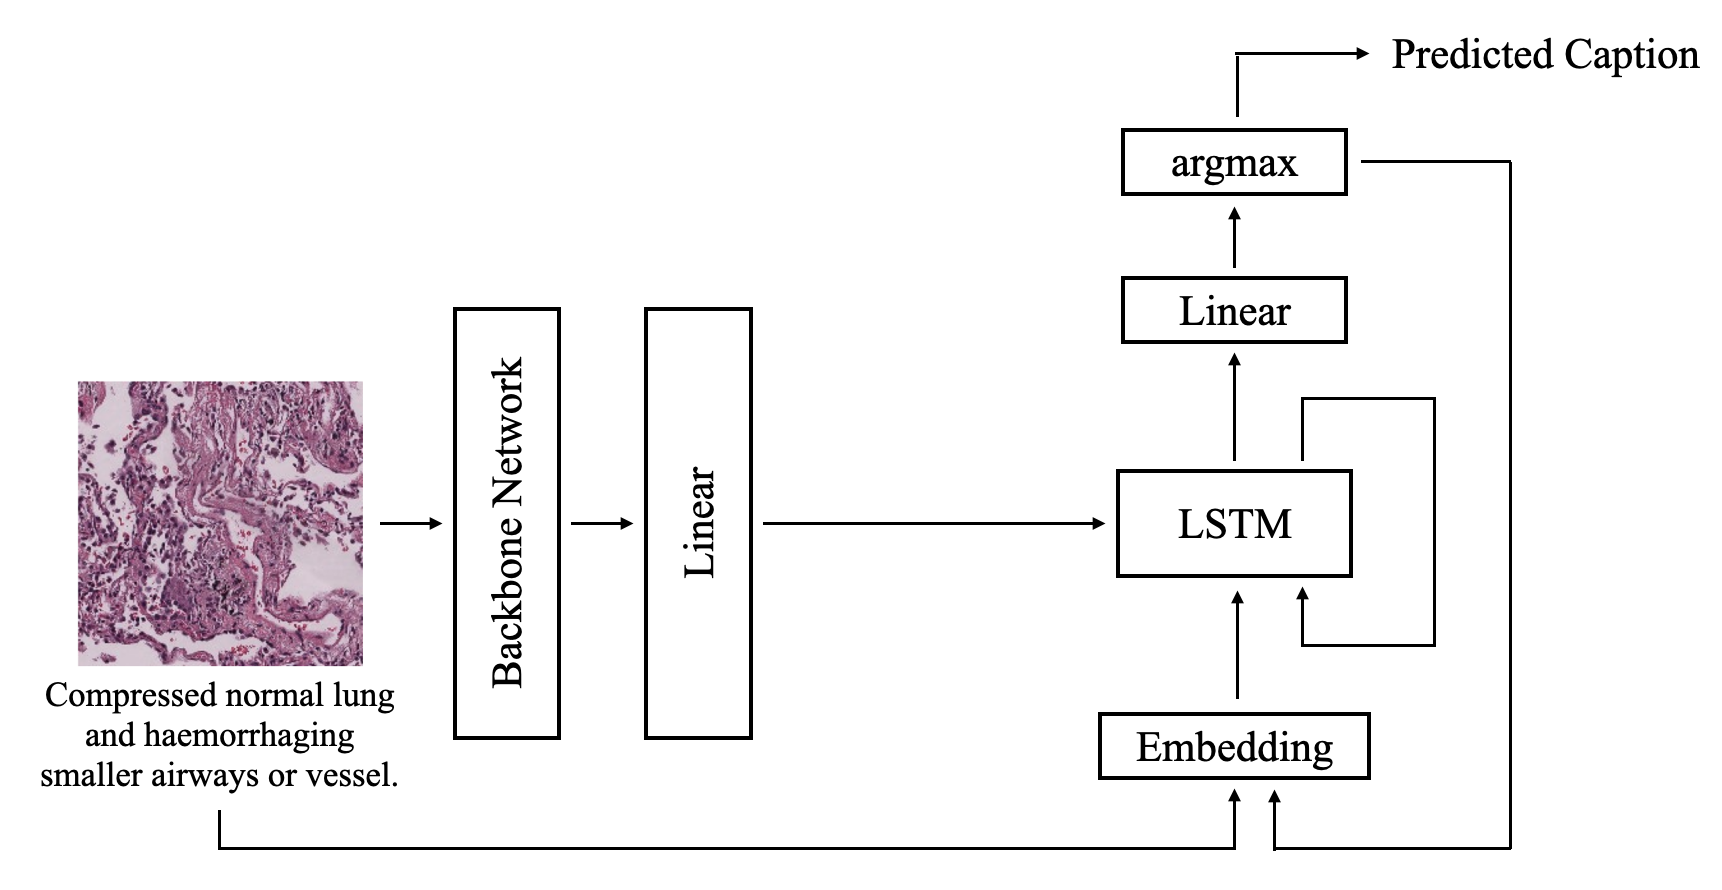
\includegraphics[width=1\linewidth]{images/lstm.png}
    \caption{Graphical representation of the tile image captioning model. The model utilises a frozen HPL backbone network, which is a CNN network trained using the Barlow Twins method. The diagram depicts the same tile shown in the previous figure, from sample TCGA-97-8179-01Z-00-DX1 of the TCGA dataset. The tile is paired with the caption ``Compressed normal lung and haemorrhaging smaller airways or vessel.'' serving as an input.}
    \label{fig:lstm-cap}
\end{figure}

\begin{figure}[h!]
    \centering
    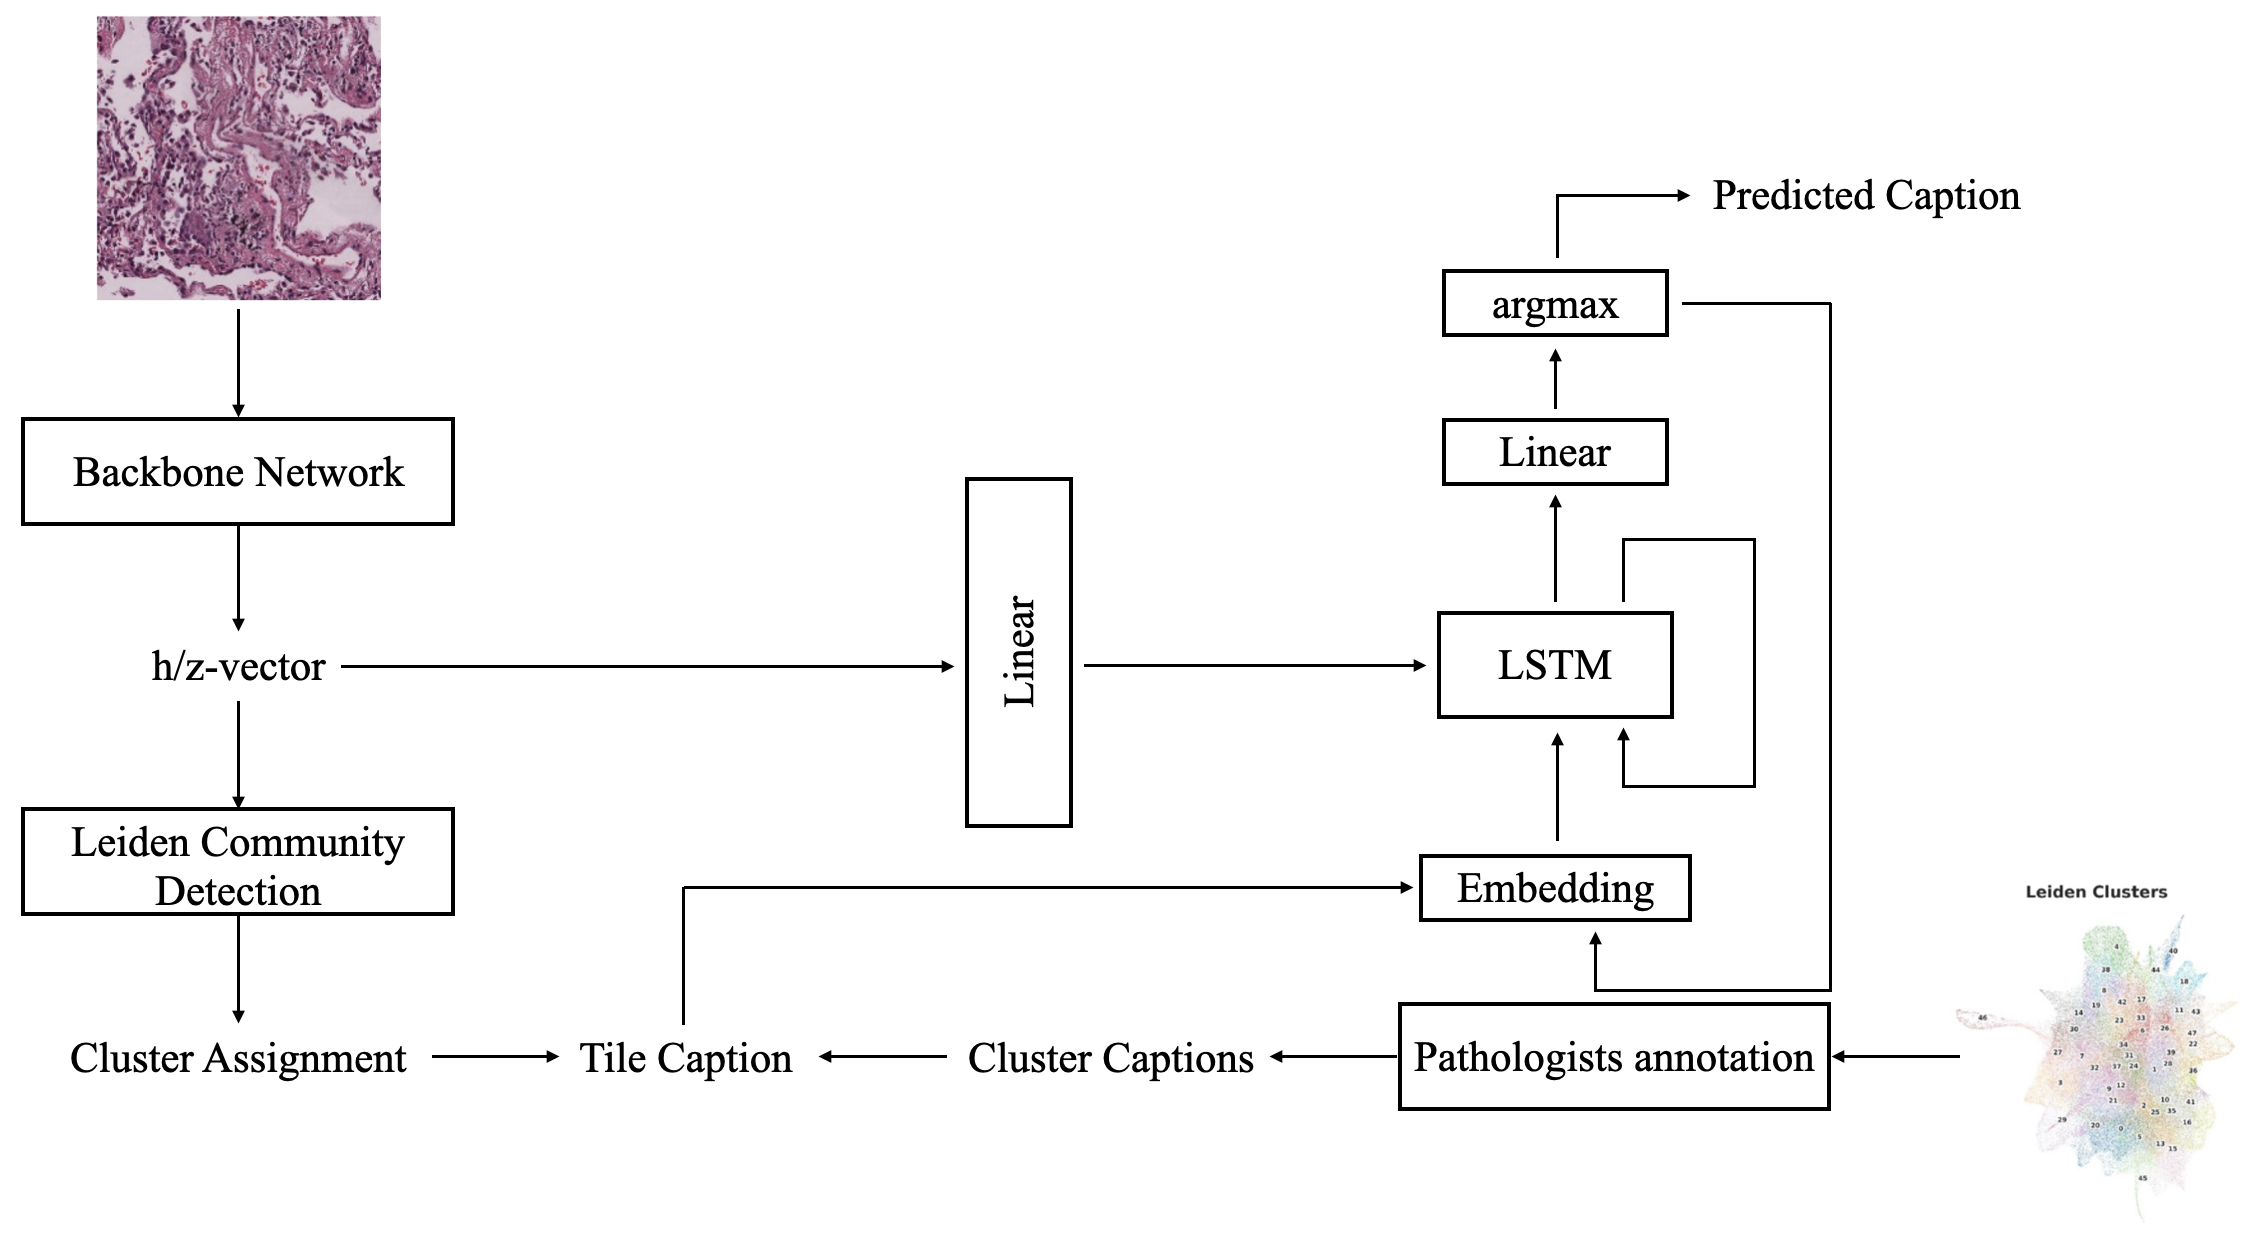
\includegraphics[width=1\linewidth]{images/full-work.png}
    \caption{Diagram illustrating the comprehensive connection between the HPL backbone network and the text captioning model. The CNN backbone network generates two types of vectors: h-vectors and z-vectors. h-vectors serve as inputs for the larger model, while the smaller model employs z-vectors. Both image representation clustering (using Leiden community detection) and the tile image captioning model share the same frozen backbone CNN network as their tile image feature encoder. The visualisation of Leiden clusters (bottom right) is adapted from the HPL paper \citep{ClaudioQuiros2024}.}
    \label{fig:workflow-full}
\end{figure}
\clearpage

The data used for training and evaluating the tile image captioning model came from the TCGA-LUAD dataset, which exclusively contained tiles from patients affected with lung adenocarcinoma. The dataset comprised 405,712 tile images\footnote{This number was after excluding some entries in the file provided by HPL's repository. For example, some samples had duplicate entries and conflicting vector values, so they were excluded. The original paper mentioned that there were around 411,000 tiles in the dataset pre-processing.}.

To decrease the required computing power and storage, we utilised the pre-processed z-vector and h-vector data of the dataset available through HPL's GitHub repository. The complete data processing and model architecture are illustrated in Figure \ref{fig:workflow-full}. We created two variants of the captioning model based on the two vectors.

The first model is a smaller variant which uses the z-vector, size 128 for hidden state and cell state of LSTM, and word embeddings of size 128. With a total of 182,018 learnable parameters, this smaller model offers better computational efficiency. This model is referred to as the z-vector LSTM model.

The second model is a larger one, using the h-vector as input, size 1024 for hidden state and cell state of LSTM, and word embeddings of size 1024. This expanded architecture encompasses 9,712,770 learnable parameters, potentially providing better performance at the cost of increased computational demands. This model is termed the h-vector LSTM model.

For both models, the image embedding serves as the input to the LSTM at the first timestep. In subsequent timesteps, the input to the LSTM is the text embedding of the previous token. This is achieved through the embedding layer (discussed in Section \ref{sec:embedding-layer}), which transforms a token into a dense vector suitable for processing by neural networks. 

\section{Training and Inferencing} \label{sec:caption-training}
Training RNNs presents a different challenge compared to traditional feedforward networks due to their recursive structure. RNN architectures have feedback loops where outputs depend on internal model states that evolve every timestep. While this allows RNNs to process sequential data effectively, it disallows the use of normal backpropagation for training. Instead, backpropagation through time (BPTT) is used to train RNNs \citep{bptt}.

The BPTT algorithm conceptually \emph{unfolds} the recurrent block as if it goes through time. Afterwards, backpropagation can be similarly applied to the model. The depiction of this unfolding is shown in Figure \ref{fig:bptt}.

\begin{figure}[t]
    \centering
    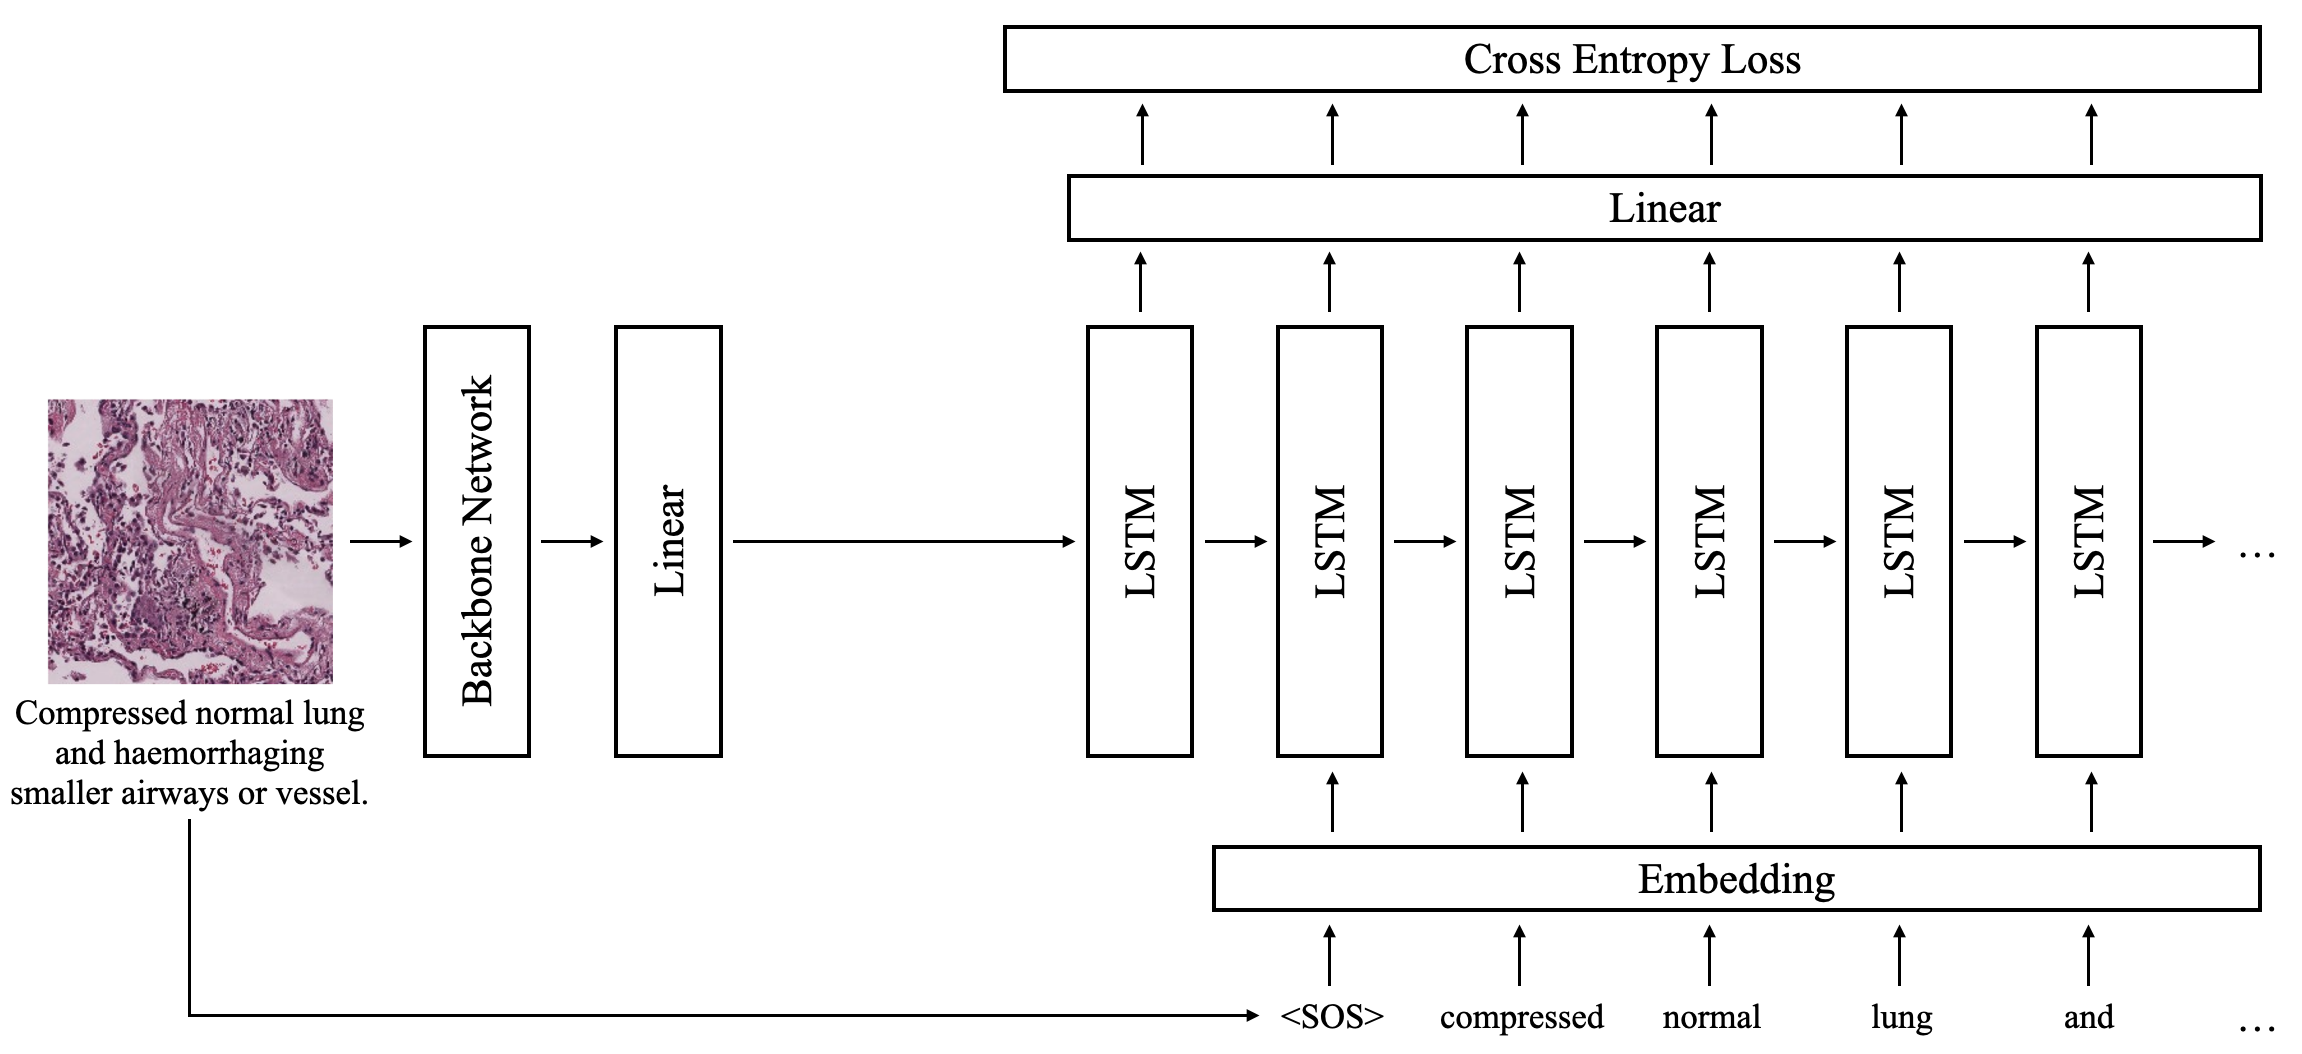
\includegraphics[width=1\linewidth]{images/bptt.png}
    \caption{Graphical representation of the LSTM block unfolding during training with BPTT. Each LSTM block in the diagram represents the same LSTM at different time steps. The expected output token for time step $t$ is used as the input for time step $t + 1$. The input for the initial time step $t=0$ is the image embedding. The diagram shows a tile from sample TCGA-97-8179-01Z-00-DX1 paired with the caption ``Compressed normal lung and haemorrhaging smaller airways or vessel.'' serving as an input.}
    \label{fig:bptt}
\end{figure}

We employed cross-entropy loss as the loss function. The model outputs the vector of probability logits for each word in the vocabulary as the next token. Cross-entropy measures the difference between the probability distribution predicted by the model and the one-hot encoded ground truth of the next token. We used Adam as the preferred optimisation method with the learning rate set at $1e-5$. 

During the inference phase, we used greedy search for caption generation. This approach involves selecting the token with the highest probability at each timestep as the next token in the sequence. While there are more sophisticated methods (discussed later in Section \ref{sec:future-work}), greedy captioning was expected to perform adequately because of the simplicity of the dataset. Figure \ref{fig:greedy} depicts the greedy caption generation process in a diagram of an unfolded LSTM block through time, analogous to Figure \ref{fig:bptt} showing unfolding in BPTT.

\begin{figure}[h!]
    \centering
    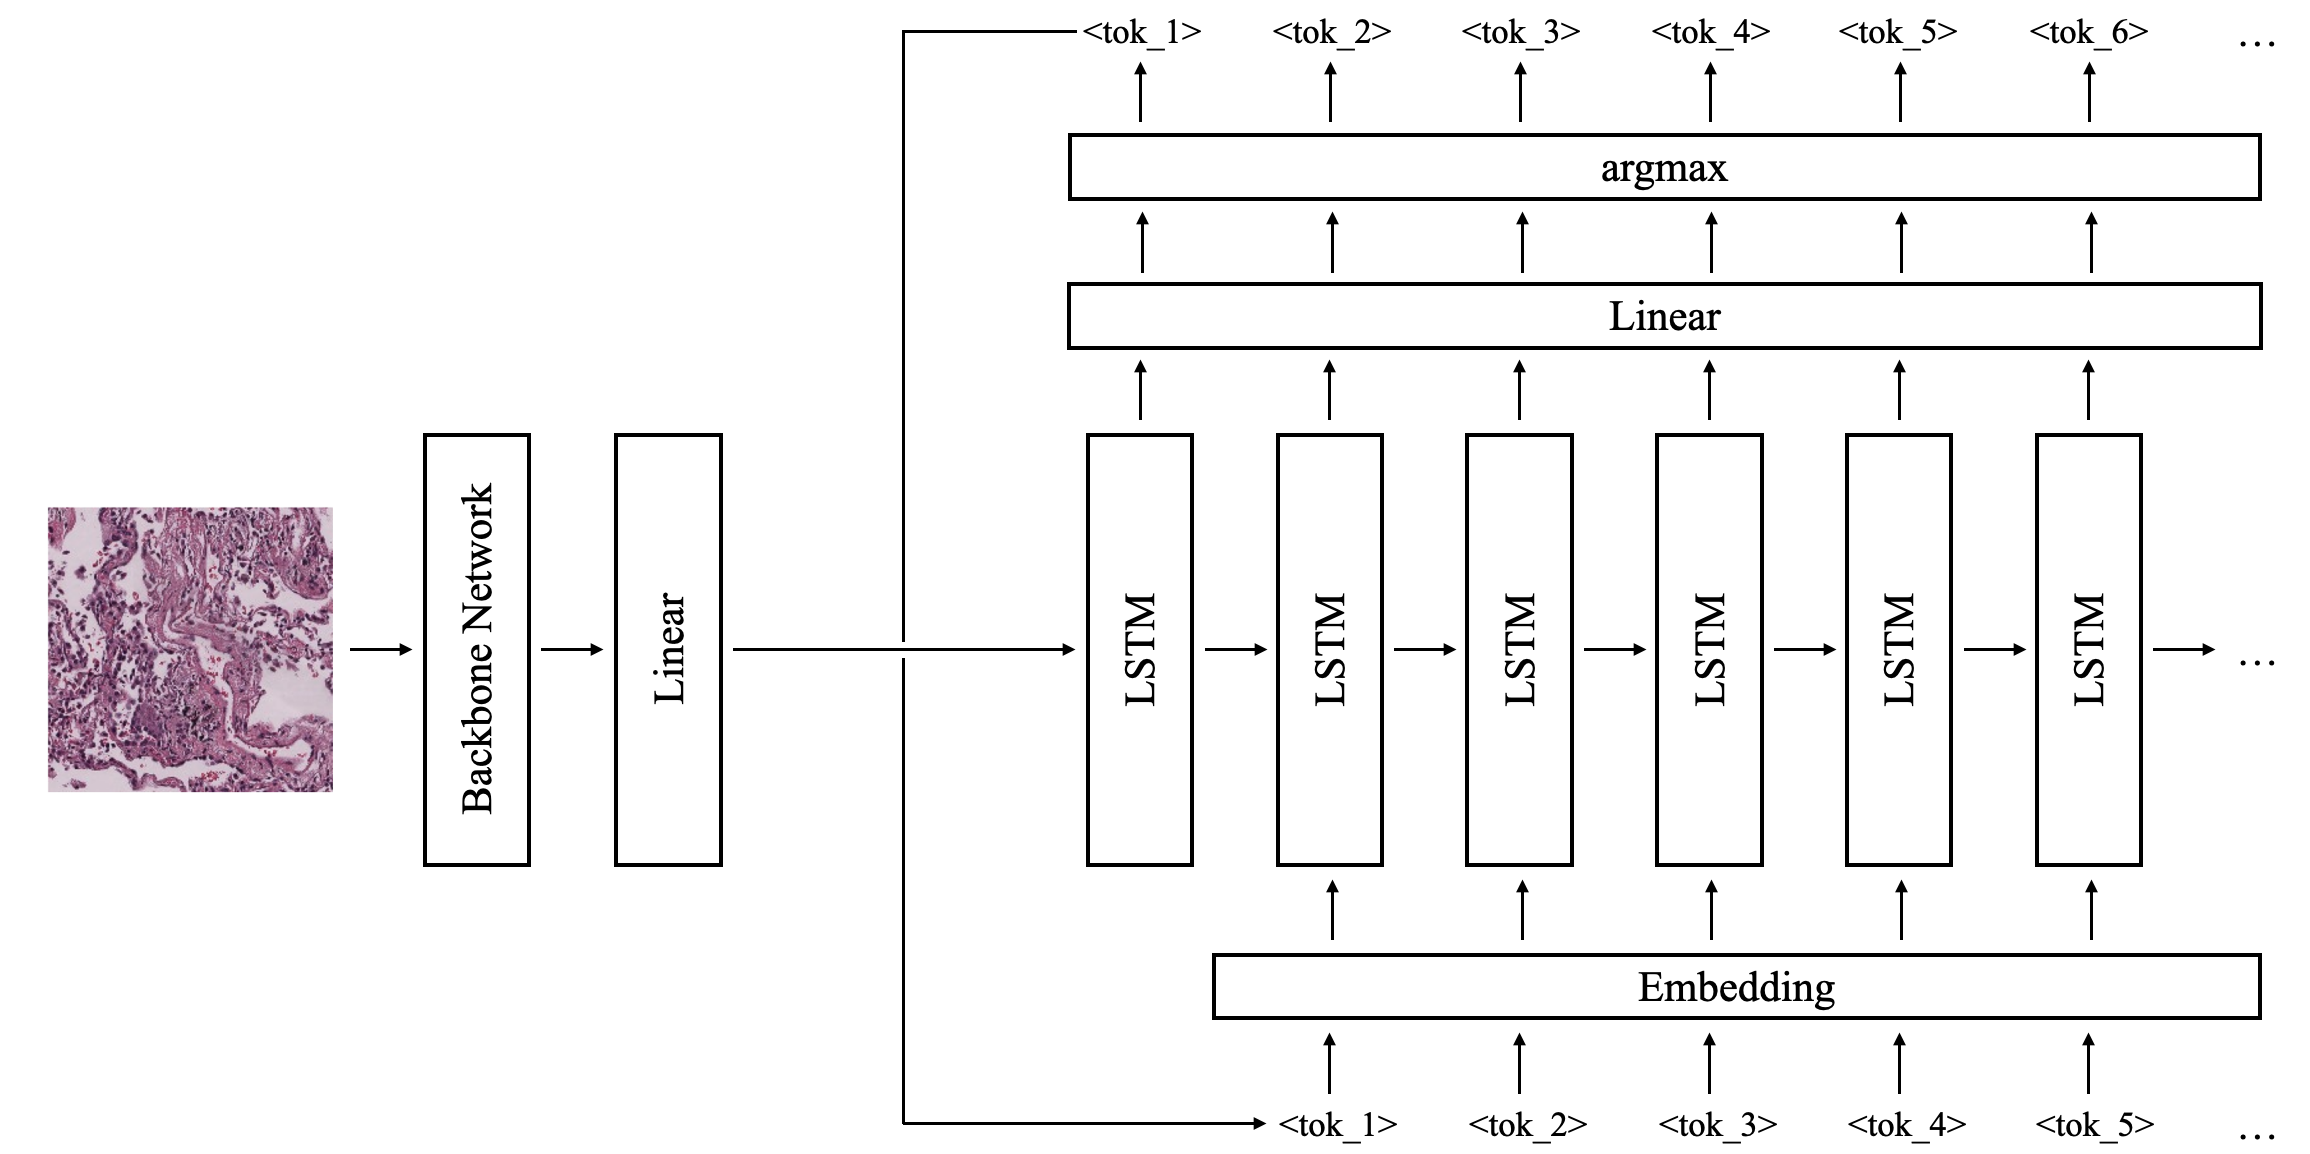
\includegraphics[width=1\linewidth]{images/greedy.png}
    \caption{Diagram of the model generating a caption for an input image using greedy search. The argmax function identifies the word in the vocabulary with the highest predicted probability at each time step. This token is forwarded to the output, and looped back as the input to the LSTM via the embedding layer for the next time step. This process repeats until a certain limit is reached, or the generated token at that time step is the special <EOS> token.}
    \label{fig:greedy}
\end{figure}

The dataset was divided into training, validating, and testing sets with a ratio of 70:10:20, respectively. Both model variants were trained on the training set for 100 epochs on 2 GPU-A100-40 nodes, for a total of 8 NVIDIA A100 GPUs, on the Tursa\footnote{https://www.epcc.ed.ac.uk/hpc-services/dirac-tursa-gpu} system. At the end of each epoch, the models were evaluated on the validating set, and the validating losses were tracked across epochs. The model parameters with the lowest validation loss over the training period were selected for final evaluation on the testing set.

\section{Evaluation Results} \label{sec:caption-results}
The complete report on the metrics from evaluating both models on the testing set is presented in Table \ref{tab:text-metrics}. Both variants of LSTM performed exceptionally well on the dataset. Based on the metrics, both models produced captions that closely matched the reference annotations. The h-vector variant slightly outperformed the z-vector counterpart across all metrics. Figure \ref{fig:caption} shows the captions generated by the h-vector LSTM model on some of the tile images in the TCGA-LUAD dataset.

\begin{table}[]
\centering
\caption{A table summarising \textsc{Rouge} and \textsc{Bleu} scores, which are used to evaluate models with natural language output. Both variants of the model scored exceptionally high on these metrics, meaning the generated captions by the model on the tile images closely resembled the reference captions. The h-vector LSTM model consistently outperformed the more compact z-vector LSTM model.}
\label{tab:text-metrics}
\rowcolors{2}{}{gray!3}
\begin{tabular}{@{}lll@{}}
\textbf{Metric}           & \textbf{z-vector LSTM} & \textbf{h-vector LSTM} \\ \midrule
\textbf{\textsc{Bleu-4}}  & \textbf{0.930}               & \textbf{0.952}                \\ \rule{0pt}{3ex}
\textbf{\textsc{Rouge-L}} & \textbf{0.962}               & \textbf{0.974}                \\
Precision                 & 0.962                        & 0.974                         \\
F1                        & 0.960                        & 0.972                         \\ \rule{0pt}{3ex}
\textbf{\textsc{Rouge-1}} & \textbf{0.963}               & \textbf{0.974}                \\
Precision                 & 0.963                        & 0.974                         \\
F1                        & 0.961                        & 0.973                         \\ \rule{0pt}{3ex}
\textbf{\textsc{Rouge-2}} & \textbf{0.942}               & \textbf{0.960}                \\
Precision                 & 0.942                        & 0.960                         \\
F1                        & 0.941                        & 0.960                        
\end{tabular}
\end{table}

\section{Discussion} \label{sec:caption-discussion}
The CNN-RNN tile image captioning model demonstrates the viability of the workflow introduced in Section \ref{sec:data-workflow} to efficiently generate tile-level annotations. The workflow can streamline the human annotation process, enabling the assignment of diverse annotation types --- not limited to textual annotation --- to each individual tile.

This approach addresses one of the fundamental challenges in histopathological image analysis: the lack of high-quality tile-level annotations. The workflow has the potential to accelerate research in this field by facilitating supervised learning of models on histopathology slide images.

In this study, we built the downstream model (the CNN-RNN captioning model) as tied to the original model by sharing the same image feature encoder (CNN). This was by choice and not by necessity. This choice was primarily made to save on computing power and storage. In future applications, the downstream model can use a completely different CNN tailored to specific downstream tasks.

The efficacy of this workflow is critically dependent on the quality of the generated tile-level annotations. Since cluster-level annotation is inherited by each member of that cluster, the quality depends on the \emph{purity} of the HPCs. Each HPC should consistently and purely contain one type of histomorphological landscape, so the cluster annotations are applicable to all member tiles.

As previously discussed in Section \ref{sec:dropout}, the approach of clustering visually similar tiles as in the HPL methodology appears to work better within a single tissue context. Applications requiring tile-annotation pairings across multiple tissue types may benefit from implementing this workflow separately for each tissue source. However, this will come at an increased cost of annotation.

Other methods to ensure the quality of the annotations should be employed. For instance, employing multiple independent annotators and measuring inter-annotator agreement can indicate the consistency of the annotation process \citep{Artstein2017}. In the context of this framework, low agreement levels may indicate low purity of HPCs. 

It is important to consider the performance metrics under the context of this study's dataset. The exceptional results should be interpreted with the consideration that the dataset is relatively limited in scale and diversity. For comparison, mPLUG's \textsc{Bleu-4} score on captioning images in the COCO captions dataset was 0.465 \citep{mplug}. mPLUG is the state-of-the-art model at the time of writing. We can explain the lower score of mPLUG by the fact that the COCO captions dataset is substantially more diverse than the dataset employed in this study. Therefore, it is best to avoid a direct comparison of performance metrics.

One limitation of the evaluation approach is that the automated metrics, \textsc{Bleu} and \textsc{Rouge}, only consider the difference between the model's output and the generated annotation. It does not measure how well the generated annotation matches with the paired tissue tile image. A separate quality assurance workflow or evaluation of annotation quality must be employed for a comprehensive evaluation.

Nevertheless, the results in this study show that an effective downstream model can be developed using tile-annotation pairings derived from HPL methodology. However, further refinements to the captioning model architecture would be necessary for larger-scale applications. This is discussed in Section \ref{sec:future-work}.

\begin{figure}[h!]
    \centering
    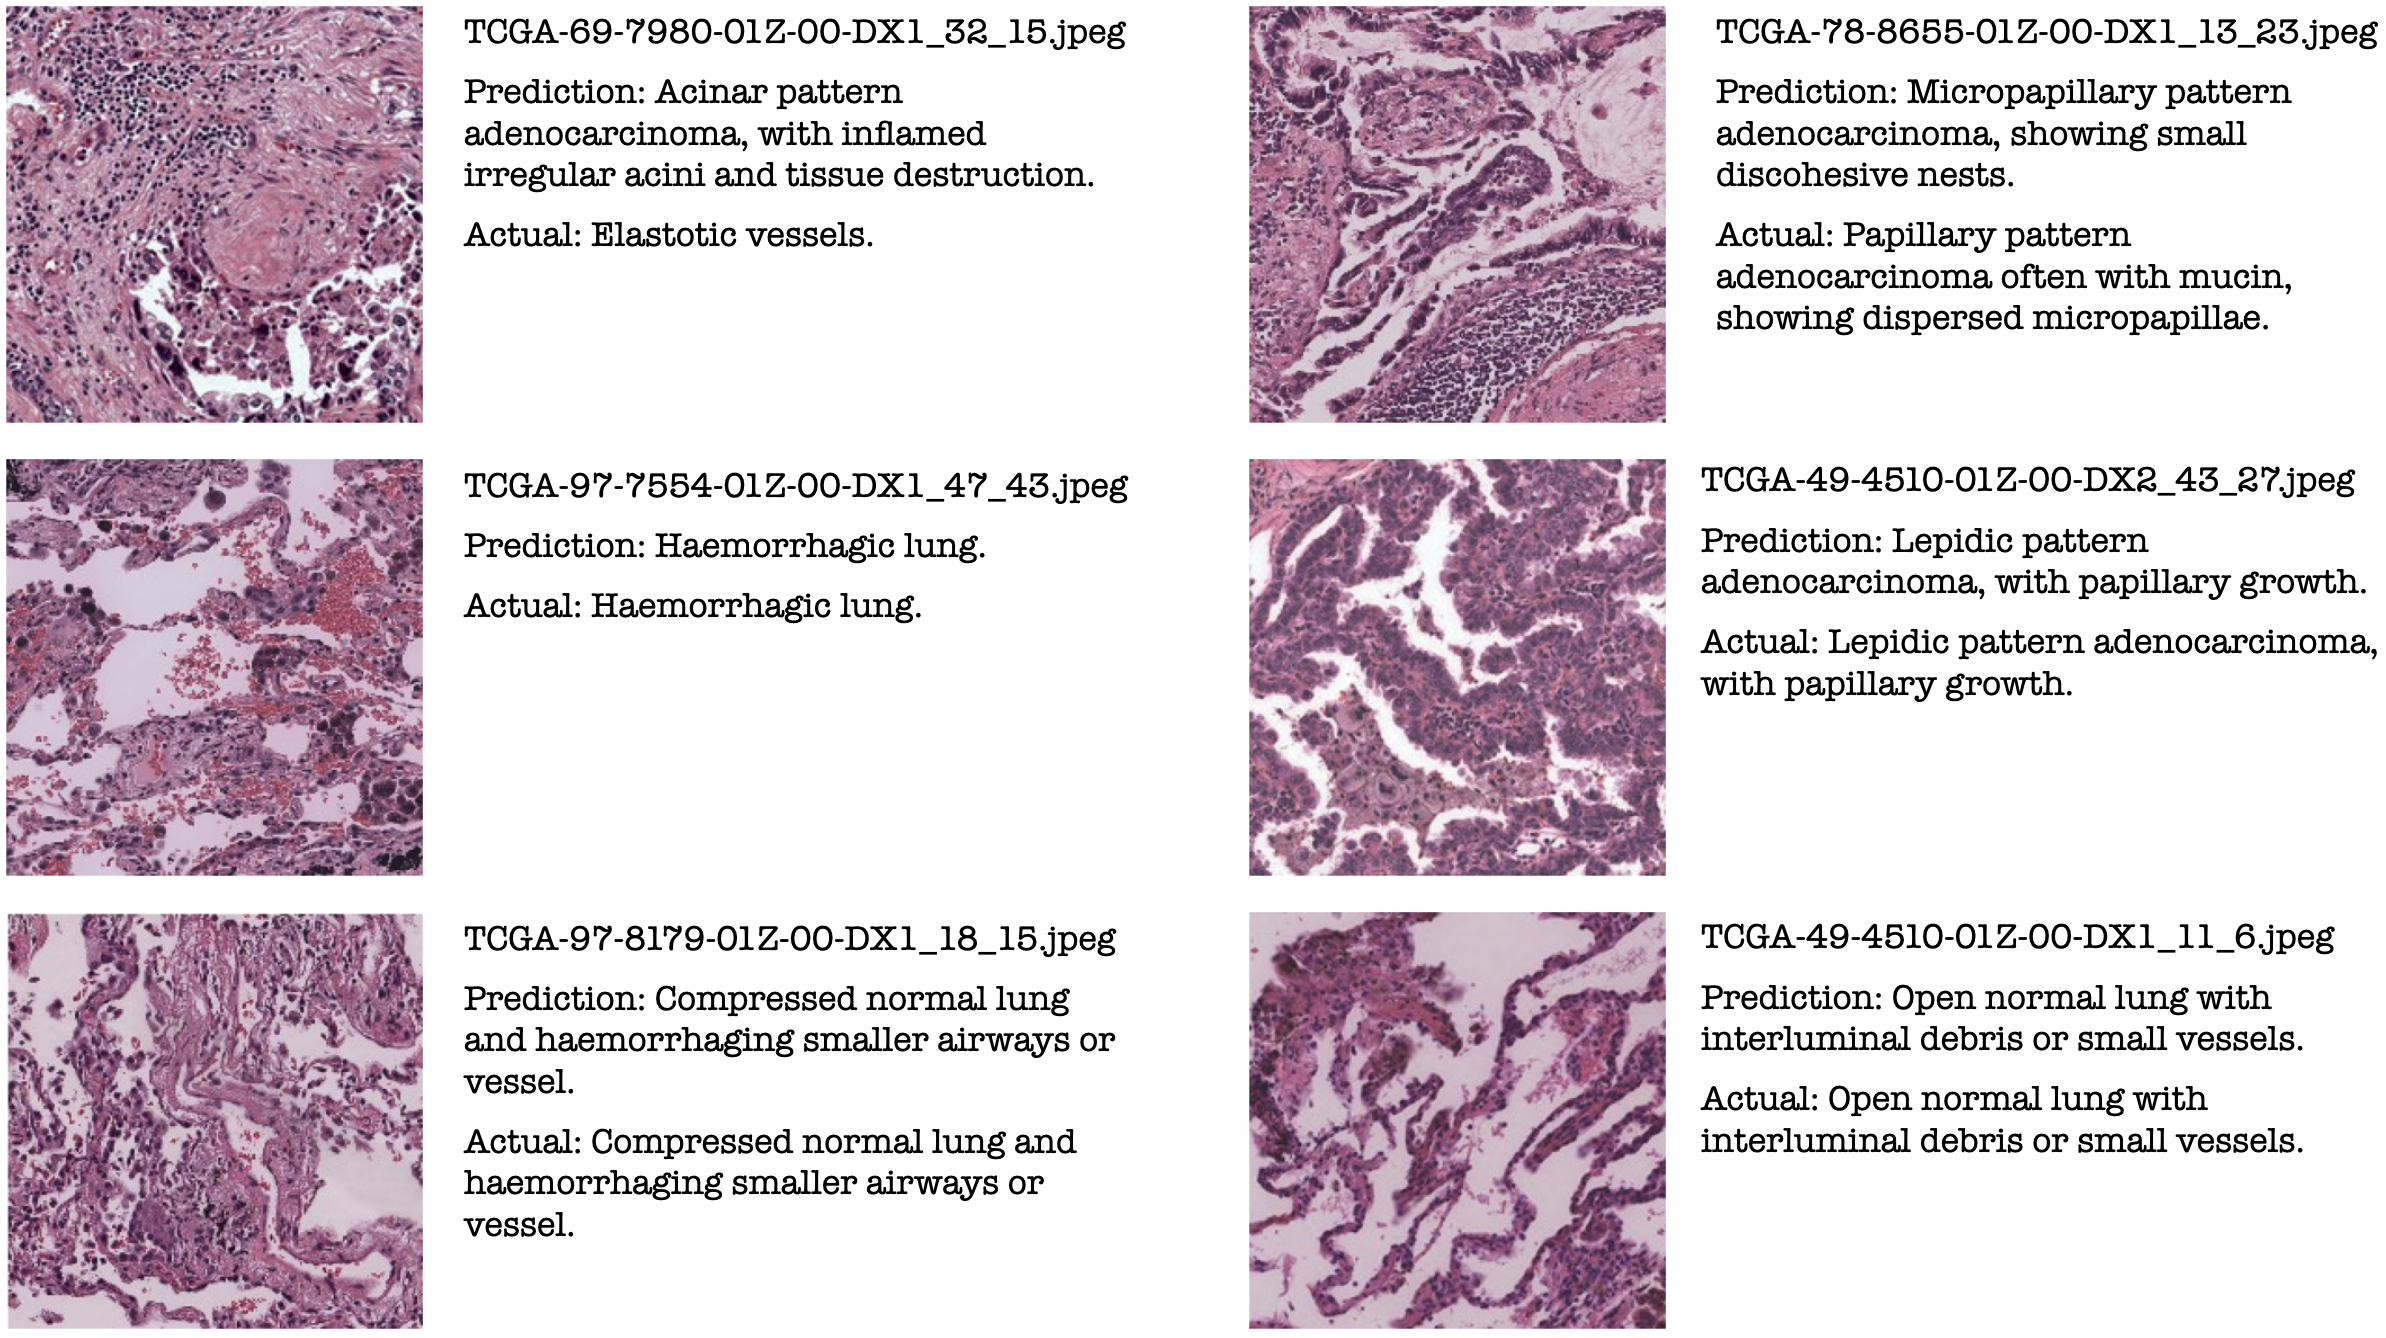
\includegraphics[width=1\linewidth]{images/caption.png}
    \caption{Selected tile images from TCGA-LUAD dataset, alongside the corresponding predictions generated by the h-vector LSTM model and the actual paired annotations produced by the workflow described in Section \ref{sec:data-workflow}. These samples were deliberately selected to show some errors by the model.}
    \label{fig:caption}
\end{figure}

%==================================================================================================================================
\chapter{Conclusion}    

\section{Summary}
This dissertation addresses two distinct but interconnected research questions. The first question involves developing a model for classifying WSIs into appropriate cancer types by using their deep representations. The second question covers using HPL methodology to generate tile-annotation pairings for training a model that could generate descriptive captions for individual tissue tile images.

Five classifier variants using WSI vectors as their inputs were implemented and evaluated. We found that the leaky version of the MLP model, called LeakyPanCancerClassifier, demonstrated marginally better performance. However, the performance differences between the various models were not significant.

The leaky MLP performed decently well on the TCGA dataset, achieving the top-1 accuracy of 0.689, top-3 accuracy of 0.899, and AUROC of 0.947 through 5-fold cross-validation. Notably, there was a contradiction between slightly low top-1 accuracy and high AUROC. This discrepancy suggested that while the model could effectively learn patterns within the WSI vector and assign probability distribution decently well, the correct class frequently failed to reach the top of the probability ranking. This interpretation is further supported by the robust top-3 accuracy.

All classifier models performed markedly worse when evaluated on external datasets collected from non-TCGA sources, specifically CMB and CPTAC. The reason for decreased performance was hypothesised to be significant differences between slides from different sources. Two primary factors likely contributed to this variation: first, the external dataset did not have inclusion criteria as strict as the TCGA dataset; second, there were some inconsistencies in slide preparation across sources. This finding highlights the importance of utilising data from multiple sources during model development to ensure robustness.

The classifier models trained exclusively on cancerous samples were evaluated using the GTEx dataset, which contains only normal tissue WSIs. The performance metrics on this OoD test were close to those observed with the evaluation with the external dataset. We concluded that, since the training dataset consisted only of primary tumour WSIs, the models might have inadvertently learnt to classify cancer types based on the normal tissue context rather than tumour-specific features.

Further analysis of OoD testing revealed systematic confusion between particular classes. Namely, cervix WSIs were misclassified as prostate, and skin WSIs as breast. The SHAP values for these classes were investigated, and the HPCs responsible for the feature values were examined. The investigation indicated the presence of noise or impurities within each cluster. A HPC appeared to contain multiple types of tissue structures that shared certain visual similarities. This implied that the clustering process was too coarse because the Leiden resolution hyperparameter was set lower than optimal. These results highlight the significant impact of hyperparameter settings in HPL methodology on downstream applications.

In the study, tiles assigned to the same HPC consistently represented one single histological structure when derived from the same tissue. This cohesion diminished when examining tiles from the same HPC but originating from different tissues. This observation leads to the conclusion that clustering with morphological appearances of the tile is more effective when constrained within a single tissue context.

One main challenge in histopathological image analysis research is the scarcity of data. In particular, quality tile-level annotations are very rare. This is due to the cost and manpower of expert pathologists required to create such datasets. Existing approaches circumvent this by using WSI-level labels as weak labels, or using methods that require no labels such as self-supervised or unsupervised learning methods.

We propose a workflow to efficiently create tile-level annotations by leveraging the clustering framework from HPL. HPCs can be annotated by human experts, and the cluster annotations can propagate back to their respective members. This approach streamlines the annotation process, creating tile-annotation pairs suitable as a dataset for supervised training of downstream models.

To validate this workflow, we built a tile captioning model using a CNN-RNN architecture. The CNN is used as a feature extractor to extract features from the tissue tile images, transforming them into dense feature vector representations. These feature vectors are subsequently processed by the RNN, functioning as a text decoder for generating appropriate captions. The pre-trained backbone model from HPL methodology was employed as the feature extractor. The text decoder followed the LSTM architecture, which translates the extracted visual features into natural language captions.

Two variants of this architecture were developed and evaluated: a more compact model that utilises the 128-dimensional z-vector from the backbone network, and a larger model that uses the 1024-dimensional h-vector with correspondingly bigger hidden layers and internal states.

Both models performed exceptionally well on the TCGA-LUAD dataset, with the h-vector LSTM model performing better on all metrics by a small margin. On the testing set, the h-vector LSTM model attained a \textsc{Bleu-4} score of 0.952, and a \textsc{Rouge-L} score of 0.974. 

While these performance metrics appear remarkably high, they must be interpreted within the context of the dataset's limited scope and diversity. There were only as many variations of captions as there were numbers of HPCs from the data provided by HPL, totalling 46 unique clusters. The size of the vocabulary was similarly limited at 130 unique tokens.

The efficacy of this workflow is critically dependent on the annotation quality, which in turn is dependent on the cluster purity. For larger-scale applications, additional measures must be employed to ensure and evaluate the quality of the tile-annotation pairings.

Nonetheless, the models successfully demonstrate the viability of the proposed workflow. This approach can provide access to high-quality tile-level annotations, which may just be the catalyst needed for breakthroughs in the field of histopathology image analysis.

\section{Reflection}
Machine learning and model training are very resource-hungry. Several design choices and decisions are made based on limitations in either computing power or storage. It may be better to secure these early to create better models.

Working with WSIs in particular makes storage a real issue. Raw WSI datasets reach terabytes in size, which is beyond the scope I can comfortably provide. Furthermore, this means that making backups is virtually impossible, as accommodating one copy is already arduous. I was unlucky enough to have a storage fault, which set the progress back by quite a bit. Thankfully, there was no second fault. I, however, learned to split the project into multiple parts, and back up the parts that I can.

This is an extremely fast-moving field, and it can be hard to find where to go and where to look. Reading publications can cause real information overload, and I got lost in the sea of information quite a number of times. I found that, usually, it is better to start small, very small. Rather than trying to start by building a gigantic model, maybe just knowing how to rotate a tensor is a more tangible goal, and work my way up from there.

Applying machine learning to other fields requires both computer science knowledge and domain knowledge for the application. I found myself picking up medical textbooks a number of times (more than I would like) while working on this project. However, I think it would be much harder to research this while seeing H\&E slides as nothing but smudges of pink ink.

Looking back, I think this was a challenging project. There were moments of frustration when it seemed like nothing would work, funny moments when I got stuck on a bug for an hour just because I made one typo, and moments of joy when the model finally trained properly. All in all, this was an enjoyable project to work on, and it provided me with valuable hands-on experience as a machine learning engineer.

\section{Future work} \label{sec:future-work}
Several points of discussion may benefit from additional resources:
\begin{itemize}
    \item Section \ref{sec:external} presents the results of assessing the classifier models on the external dataset. However, the dataset did not cover all the cancer types supported by the classifier due to the limited availability of publicly accessible cancerous WSIs. Access to more data would enable a more comprehensive analysis and potentially yield more robust results.
    \item In Section \ref{sec:discuss-classifier}, the dissertation mentions that the clustering approach as in HPL methodology performs better when limited to a single tissue context. However, we were limited by insufficient computing power and storage to process large volumes of data and limited access to histopathological expertise to interpret data comprehensively.
    \item Section \ref{sec:caption-discussion} mentions that the automated evaluation approach can only measure differences between the predictions and annotations generated from the workflow. We did not possess the method or resources to quantify the mismatch between the generated annotations and the tile images.
\end{itemize} 
Collaboration with a team of histopathologists could allow a more in-depth analysis of tile-annotation mismatch. Extra computing power and storage capacity can facilitate processing larger datasets. While the points discussed in the dissertation are noteworthy findings, they are constrained by a number of resource limitations. Additional resources can further substantiate the results, with more rigorous analyses based on a larger number of samples.

The workflow in Section \ref{sec:data-workflow} can be branched out to create more models. As the method is not limited to textual annotations, it may be interesting to see what kinds of models we can build with tile-level annotations.

The tile image captioning data can be extended to cover more cancer types, or more histopathological appearances. However, this may require improvements to the model architecture:
\begin{itemize}
    \item Another CNN encoder can be fine-tuned for the specific purpose of histopathological tile image captioning.
    \item Greedy search is by no means optimal. Beam search with beam width of 3 or 5 is consistently found to be superior to greedy search \citep{cohen2019, kumar2022}.
    \item A pre-trained text vectorisation model can be integrated in-place of the embedding layer. These models are trained to embeds a token into a knowledge representation vector. This means that words with similar meaning will be close to each other in the knowledge space.
    \item The current state-of-the-art model for NLP tasks employs the transformer architecture \citep{vaswani2023}. The LSTM text decoder therefore can be replaced with a transformer to possibly increase performance.
    \item From prior discussions, it is established that sometimes morphology alone does not convey enough information. Tissue context is also important. Therefore, when the model scaling up to include multiple tissues, it may be beneficial to do feature engineering, by including tissue source information in the feature vector.
\end{itemize}

\section{Data Usage Acknowledgements}

The results shown here are in part based upon data generated by the TCGA Research Network: \url{https://www.cancer.gov/tcga}.

A part of the data used in this publication was generated by the National Cancer Institute’s Cancer Moonshot Biobank:
\begin{itemize}
    \item CMB-BRCA \citep{cmb-brca}
    \item CMB-PCA \citep{cmb-pca}
\end{itemize}

A part of the data used in this publication was generated by the National Cancer Institute Clinical Proteomic Tumor Analysis Consortium (CPTAC):
\begin{itemize}
    \item CPTAC-COAD \citep{cptac-coad}
    \item CPTAC-LUAD \citep{cptac-luad}
    \item CPTAC-LSCC \citep{cptac-lscc}
    \item CPTAC-CM \citep{cptac-cm}
    \item CPTAC-UCEC \citep{cptac-ucec}
\end{itemize}

The Genotype-Tissue Expression (GTEx) Project was supported by the Common Fund of the Office of the Director of the National Institutes of Health, and by NCI, NHGRI, NHLBI, NIDA, NIMH, and NINDS. The data used for the analyses described in this paper were obtained from the GTEx Portal on 01/01/2025.


%==================================================================================================================================
%
% 
%==================================================================================================================================
%  APPENDICES  

\begin{appendices}

\chapter{Additional Tables}

\begin{table}[h]
\centering
\caption{Recall, precision, F1 score, and AUROC metrics from testing the classifier models on the external dataset. The arithmetic means of the metrics were calculated using only the 7 classes that were present in the external dataset. These numbers may not fully represent overall model performance due to the absence of certain class representations.}
\label{tab:ext-macro}
\rowcolors{2}{}{gray!3}
\begin{tabular}{@{}lllll@{}}
\textbf{Model Name}                 & \textbf{Recall} & \textbf{Precision} & \textbf{F1} & \textbf{AUROC} \\ \midrule
PanCancerLogisticRegression         & 0.389           & 0.492              & 0.410       & 0.793          \\
PanCancerClassifier                 & 0.418           & 0.499              & 0.437       & 0.814          \\
LeakyPanCancerClassifier            & 0.449           & 0.544              & 0.472       & 0.827          \\
PanCancerClassifierWithDropout      & 0.353           & 0.466              & 0.373       & 0.796          \\
LeakyPanCancerClassifierWithDropout & 0.422           & 0.501              & 0.440       & 0.816         
\end{tabular}
\end{table}

\begin{table}[h]
\centering
\caption{Top-k accuracies (k = 1, 3, 5) for each model on the GTEx dataset. The performance metrics on the GTEx dataset were comparable to those on the external dataset, indicating similar model performance across two datasets. Note that accuracies were calculated using the mapped labels.}
\label{tab:GTEx-results}
\rowcolors{2}{}{gray!3}
\begin{tabular}{@{}llll@{}}
\textbf{Model Name}                 & \textbf{Top-1 Acc} & \textbf{Top-3 Acc} & \textbf{Top-5 Acc} \\ \midrule
PanCancerLogisticRegression         & 0.367              & 0.777              & 0.904              \\
PanCancerClassifier                 & 0.388              & 0.739              & 0.904              \\
LeakyPanCancerClassifier            & 0.362              & 0.766              & 0.888              \\
PanCancerClassifierWithDropout      & 0.362              & 0.745              & 0.888              \\
LeakyPanCancerClassifierWithDropout & 0.367              & 0.755              & 0.904             
\end{tabular}
\end{table}

\begin{table}[h]
\centering
\caption{Recall, precision, F1 score, and AUROC metrics from testing the classifier models on the GTEx dataset. The arithmetic means of the metrics were calculated with only the 9 mapped classes, which excludes LUSC. Note that the \emph{true} label considered by these metrics were the mapped labels, which might lead to potentially misleading values.}
\label{tab:gtex-macro}
\rowcolors{2}{}{gray!3}
\begin{tabular}{@{}lllll@{}}
\textbf{Model Name}                 & \textbf{Recall} & \textbf{Precision} & \textbf{F1} & \textbf{AUROC} \\ \midrule
PanCancerLogisticRegression         & 0.395           & 0.465              & 0.313       & 0.841          \\
PanCancerClassifier                 & 0.410           & 0.501              & 0.362       & 0.840          \\
LeakyPanCancerClassifier            & 0.387           & 0.419              & 0.323       & 0.822          \\
PanCancerClassifierWithDropout      & 0.367           & 0.433              & 0.317       & 0.842          \\
LeakyPanCancerClassifierWithDropout & 0.391           & 0.468              & 0.325       & 0.847         
\end{tabular}
\end{table}

% \begin{table}[]
\rowcolors{2}{}{gray!3}
\begin{longtable}{p{0.08\linewidth} p{0.87\linewidth}}
\hiderowcolors
\caption{Textual description for each lung HPC. The descriptions were used as reference labels for image captioning. These descriptions were derived from \cite{ClaudioQuiros2024}. These captions were slightly modified to get cleaner, more natural texts than originally presented in the HPL study.} \\
\label{table:HPC-Description}
% \begin{tabular}{p{0.08\linewidth} p{0.87\linewidth}}
\textbf{HPCs} & \textbf{Descriptions} \\ \midrule   
\showrowcolors
\endfirsthead

\hiderowcolors
\caption{Continued from the previous page.} \\ 
\textbf{HPCs} & \textbf{Descriptions} \\ \midrule   
\showrowcolors
\endhead

\hiderowcolors
\multicolumn{2}{r@{}}{(cont.)} \\
\showrowcolors
\endfoot

\endlastfoot
\textbf{0}  & Acinar pattern adenocarcinoma, with inflamed irregular acini and tissue destruction.                 \\
\textbf{1}  & Inflamed compact stroma and sparse tumor. Sheets of inflammation with destruction.                   \\
\textbf{2}  & Compressed normal lung and haemorrhaging smaller airways or vessel.                                  \\
\textbf{3}  & Coarse fibrillar stroma.                                                                             \\
\textbf{4}  & Open normal lung with interluminal debris or small vessels.                                          \\
\textbf{5}  & Solid pattern adenocarcinoma with stromal TILs. Inflamed stroma. Big pleomorphic nuclei.             \\
\textbf{6}  & Adenocarcinoma with solid and sieve-like complex cribriform appearance.                              \\
\textbf{7}  & Stroma-rich solid.                                                                                   \\
\textbf{8}  & Acinar pattern adenocarcinoma, showing angulated columnar acini with multiple small branched lumina. \\
\textbf{9}  & Diverse inflamed stroma with sparse malignant epithelium.                                            \\
\textbf{10} & Haemorrhagic lung.                                                                                   \\
\textbf{11} & Adenocarcinoma, showing discohesive solid and compressed lumina or linear clefts.                    \\
\textbf{12} & Lambertosis and inflammation.                                                                        \\
\textbf{13} & Normal open lung with mild interstitial thickening and inflammation.                                 \\
\textbf{14} & Necrosis.                                                                                            \\
\textbf{15} & Solid pattern high-grade adenocarcinoma with necrosis. Patchily inflamed stroma.                     \\
\textbf{16} & Inflamed elastosis or collapsed stroma with minimal epithelium.                                      \\
\textbf{17} & Surface and margin artefacts.                                                                        \\
\textbf{18} & Cribrifrom pattern adenocarcinoma, with complex acinar or cribriform nests. Mucinous cytology.       \\
\textbf{19} & Mucinous adenocarcinoma with lepidic pattern.                                                        \\
\textbf{20} & Peribronchial fat or glands. Honeycomb appearance.                                                   \\
\textbf{21} & Acinar pattern adenocarcinoma, showing multiple compressed narrow lumina.                            \\
\textbf{22} & Large vessel lumina.                                                                                 \\
\textbf{23} & Large vessel walls.                                                                                  \\
\textbf{24} & Mucinous adenocarcinoma, showing mucin lakes.                                                        \\
\textbf{25} & high-grade solid pattern adenocarcinoma, inflamed.                                                   \\
\textbf{26} & Acinar pattern adenocarcinoma, with small angulated acini in dense cold stroma.                      \\
\textbf{27} & Micropapillary pattern adenocarcinoma, showing small discohesive nests.                              \\
\textbf{28} & Lepidic pattern adenocarcinoma, with papillary growth.                                               \\
\textbf{29} & Solid pattern adenocarcinoma with some discohesion overrun by TILs.                                  \\
\textbf{30} & Papillary pattern adenocarcinoma often with mucin, showing dispersed micropapillae.                  \\
\textbf{31} & Elastotic vessels.                                                                                   \\
\textbf{32} & Mildly fibrotic lung.                                                                                \\
\textbf{33} & Adenocarcinoma, with small nests and narrow clefts with retraction artifact.                         \\
\textbf{34} & Dense inflamed collagen.                                                                             \\
\textbf{35} & Micropapillary pattern adenocarcinoma, or tufted.                                                    \\
\textbf{36} & Inflammatory or reactive lung with interstitial expansion.                                           \\
\textbf{37} & Lepidic pattern adenocarcinoma, with acinar and papillary growth. Ragged complex appearances.        \\
\textbf{38} & Mostly solid adenocarcinoma with clear-cell change and inflammation.                                 \\
\textbf{39} & Adenocarcinoma with crowded discohesive nests appearance.                                            \\
\textbf{40} & Bronchial epithelium.                                                                                \\
\textbf{41} & Adenocarcinoma with dense stroma and small malignant nests.                                          \\
\textbf{42} & Cartilage.                                                                                           \\
\textbf{43} & Confluent lymphocytes. Sheet of inflammation.                                                        \\
\textbf{44} & Linear dark folds.                                                                                   \\
\textbf{45} & Classical cribriform adenocarcinoma.                                                                
% \end{tabular}
\end{longtable}
% \end{table}


%==================================================================================================================================

\chapter{Supplementary Figures}
\begin{figure}[h]
    \centering
    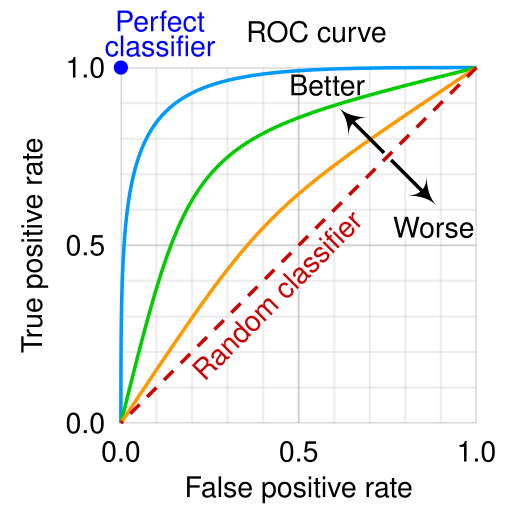
\includegraphics[width=0.5\linewidth]{images/roc_curv.png}
    \caption{Example ROC curve plot. All curves start at the bottom-left corner, where threshold is 0, and no instances are classified as positive. They end at the top-right corner, where threshold is 1, and everything gets classified as positive. A closer curve to the top-left corner indicates better performance. Image by cmglee, MartinThoma from \url{https://commons.wikimedia.org/wiki/File:Roc_curve.svg} under CC-BY-SA-4.0.}
    \label{fig:roc}
\end{figure}

\begin{figure}[h]
    \centering
    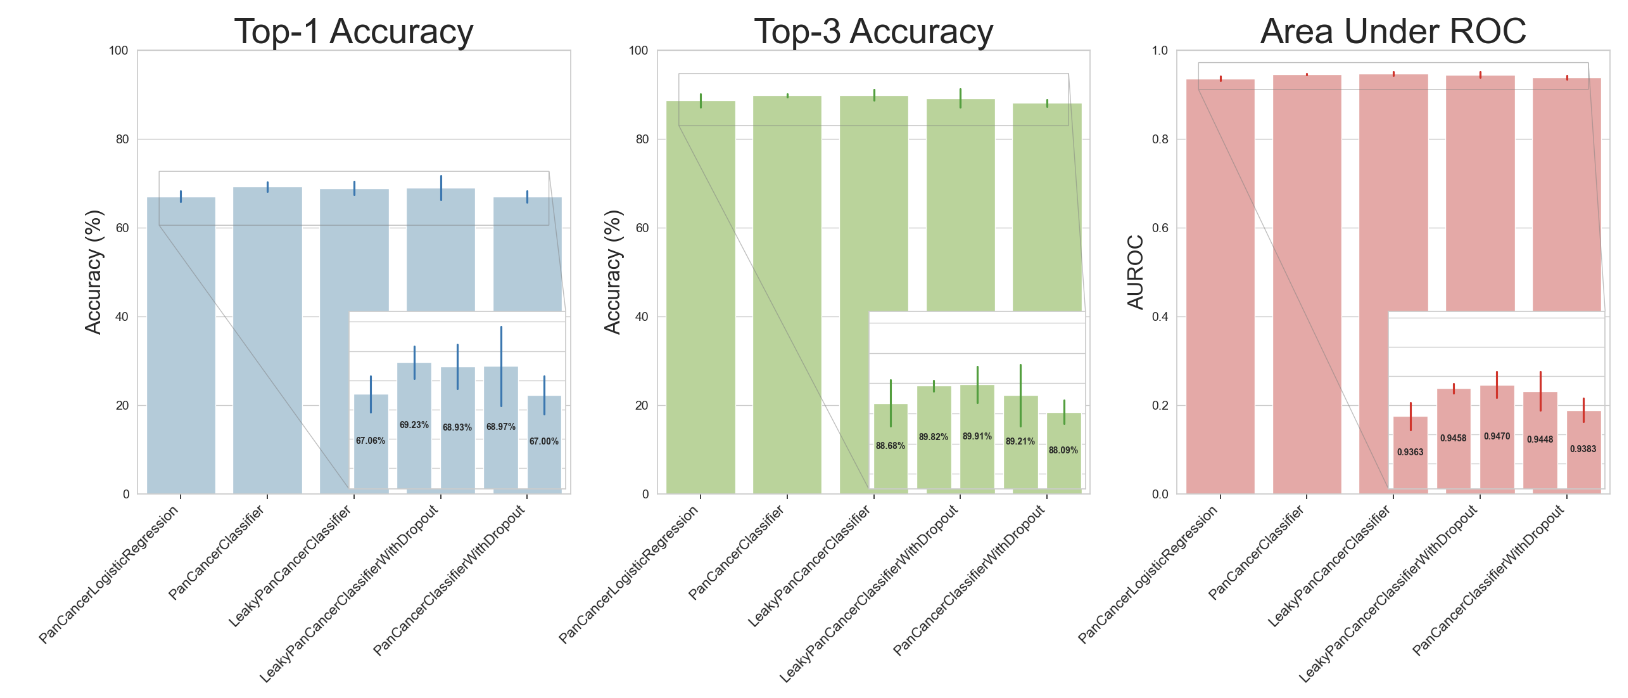
\includegraphics[width=1\linewidth]{images/CV_metrics.png}
    \caption{Bar charts for various metrics between different classifier architectures from cross-validation. The lines of top of the bars indicate error ($\pm 1SD$). The inset plots are zoom-in plots of the bar charts.}
    \label{fig:cv-barchart}
\end{figure}

\begin{figure}
    \centering
    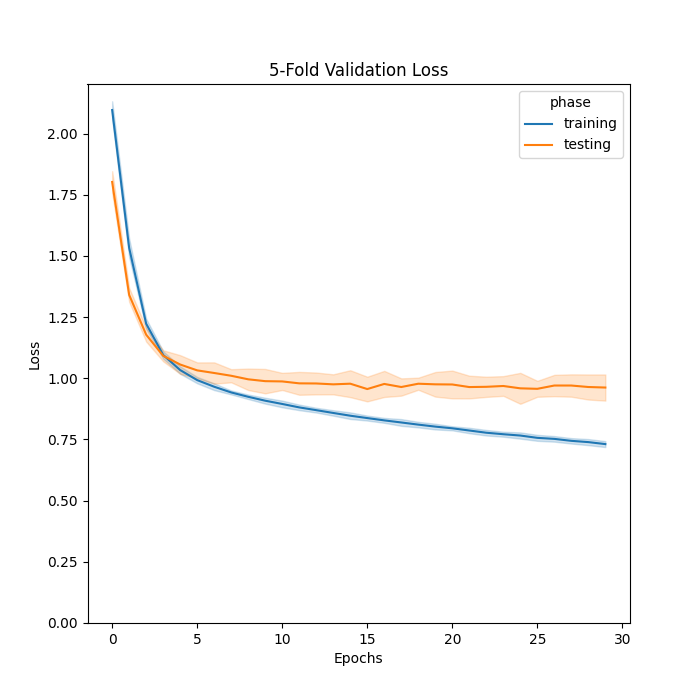
\includegraphics[width=0.75\linewidth]{images/fold_loss_curve.png}
    \caption{Line graph depicting the loss curve from 5-fold cross-validation of the LeakyPanCancerClassifier model. The model was trained for 30 epochs in each fold. The solid line shows the average loss across all folds in each epoch. The shaded regions indicate the error range ($mean\pm 1SD$). It can be seen that the model overfitted starting from around epoch 5.}
    \label{fig:fold_losses}
\end{figure}

\begin{figure}
    \centering
    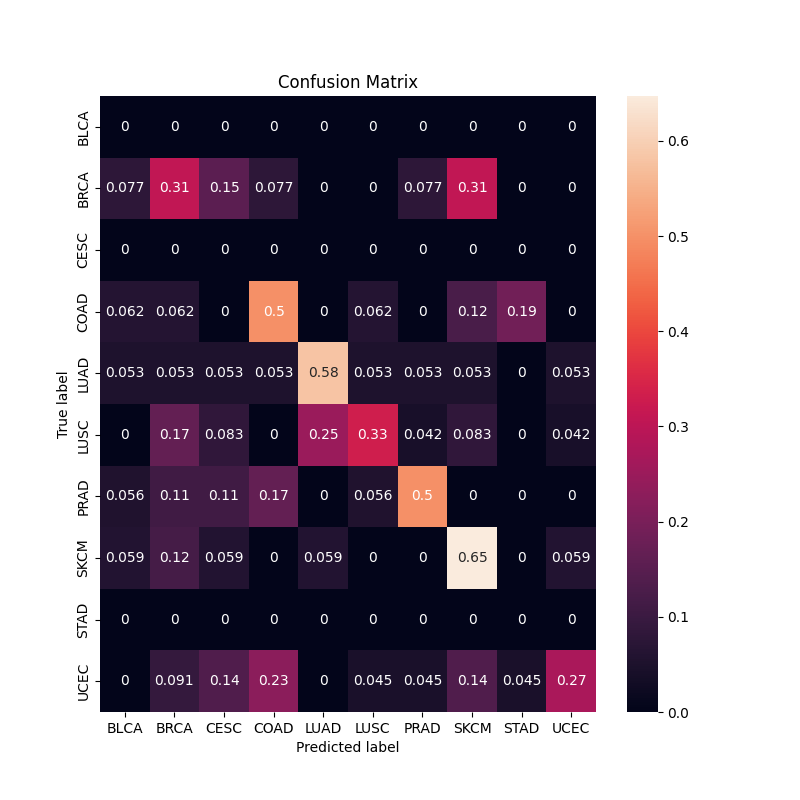
\includegraphics[width=.75\linewidth]{images/ext_conf.png}
    \caption{Confusion matrix illustrating the predictions of the LeakyPanCancerClassifier model on the external dataset. Rows corresponding to BLCA, CESC, and STAD classes contain only zero values due to the absence of these samples in the dataset. There was general confusion in the predictions, and the performance was considerably lower than the model's cross-validation results on the TCGA dataset.}
    \label{fig:ext_conf}
\end{figure}

\begin{figure}
    \centering
    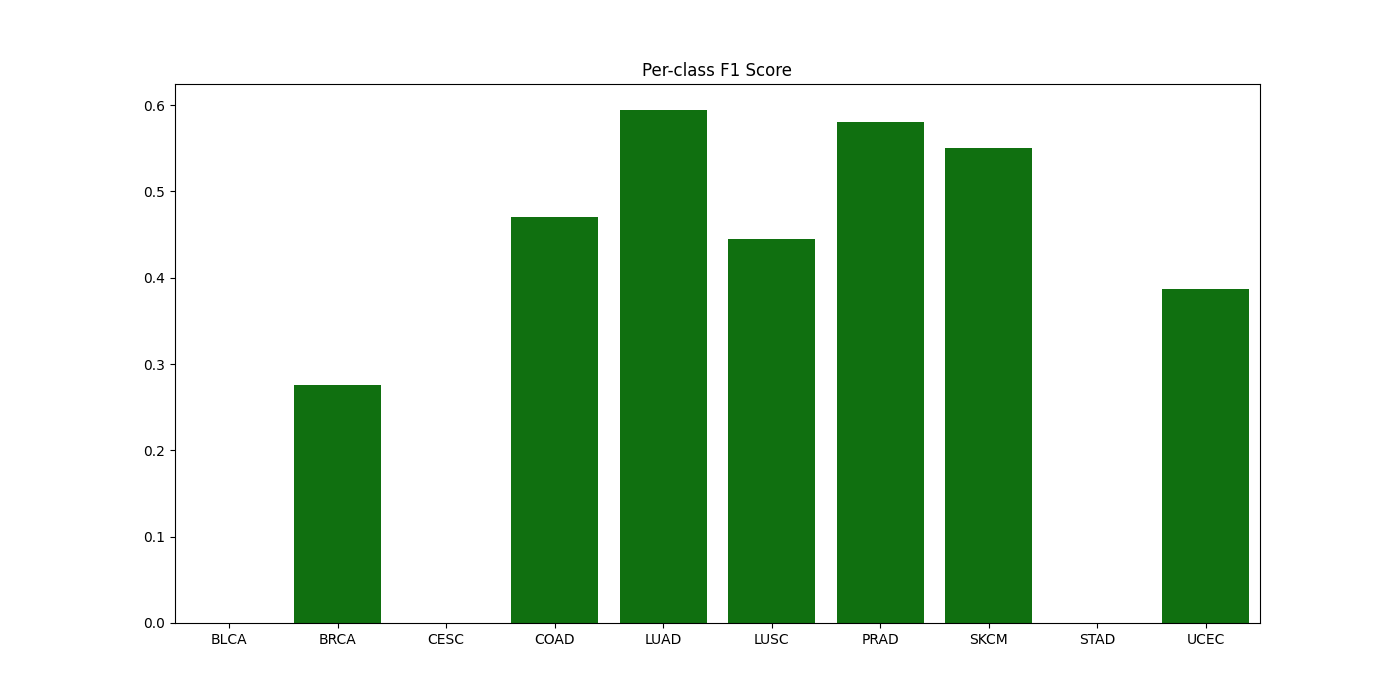
\includegraphics[width=\linewidth]{images/per_class_f1_ext.png}
    \caption{Bar chart showing per-class F1 score for predictions made by LeakyPanCancerClassifier model on the external dataset. F1 scores for BLCA, CESC, and STAD were zero due to the absence of these samples in the dataset. Per-class F1 scores aligned closely with pre-class accuracies.}
    \label{fig:class-f1-ext}
\end{figure}

\begin{figure}
    \centering
    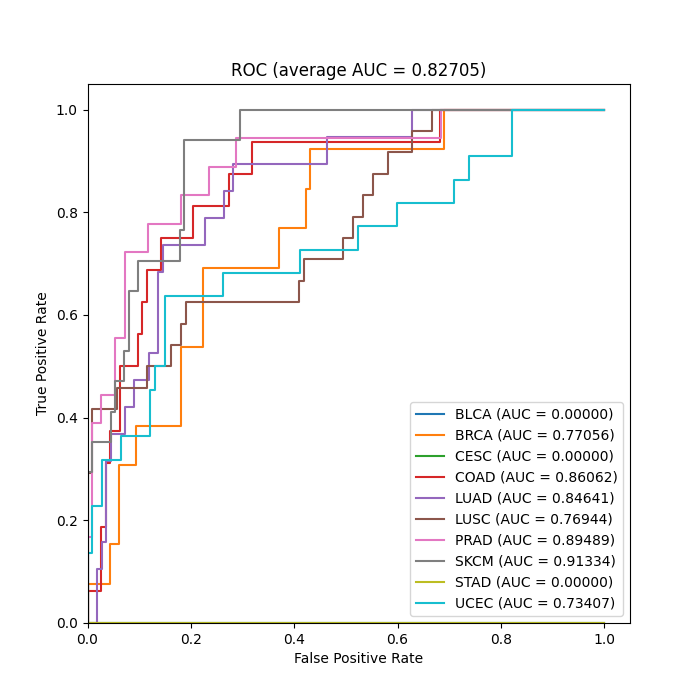
\includegraphics[width=.75\linewidth]{images/ext_roc.png}
    \caption{ROC curves illustrating the predictions of the LeakyPanCancerClassifier model on the external dataset. AUROC for classes that were absent from the dataset are listed as zero and they were excluded from calculating the overall AUROC in the title of the plot. Mediocre performance can be observed among all classes.}
    \label{fig:ext-roc}
\end{figure}

\begin{figure}
    \centering
    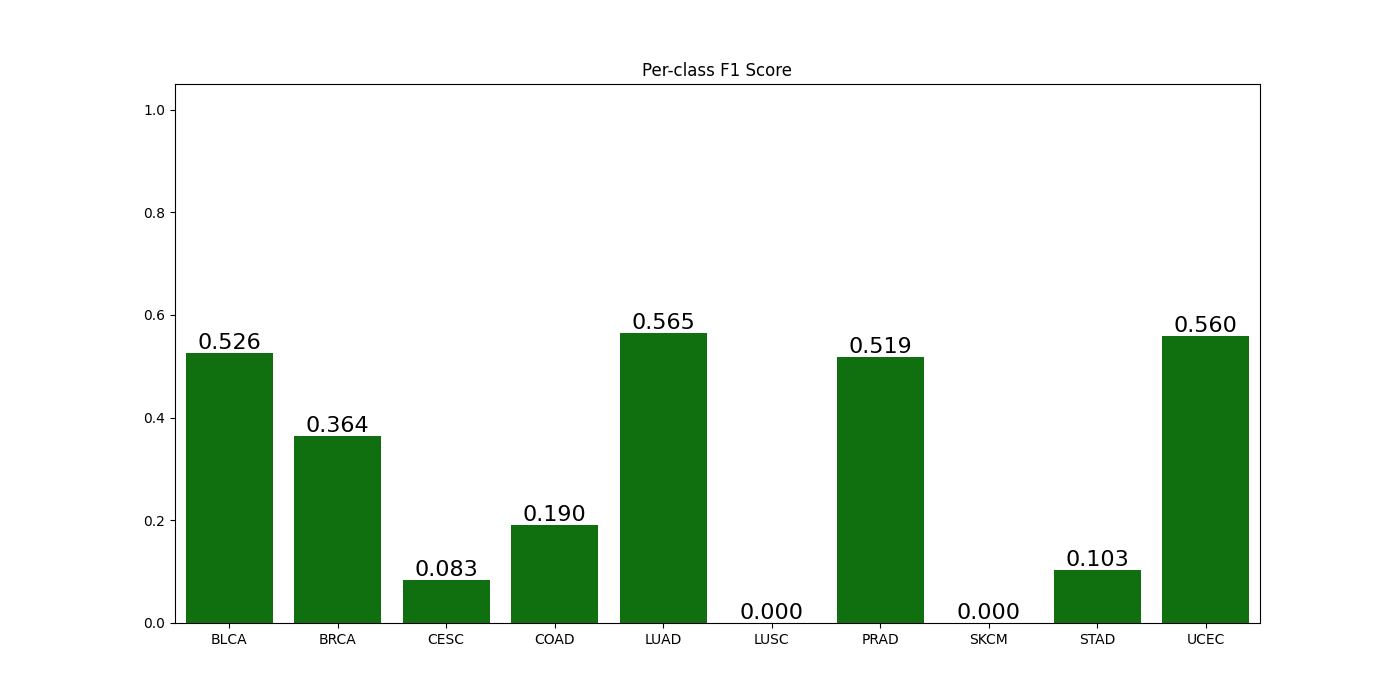
\includegraphics[width=\linewidth]{images/per_class_f1_gtex.png}
    \caption{Bar chart of per-class F1 scores for the predictions made by LeakyPanCancerClassifier model on the GTEx dataset. All lung tissue samples were mapped to LUAD, so there were no samples with LUSC label in the dataset.}
    \label{fig:class-f1-gtex}
\end{figure}

\begin{figure}
    \centering
    \includegraphics[width=1\linewidth]{images/gtex_auroc.png}
    \caption{Bar chart of per-class AUROCs for the LeakyPanCancerClassifier model's predictions on the GTEx dataset. The AUROC for LUSC was zero, as all lung samples were mapped to LUAD.  The model's performance, as indicated by AUROCs, was comparable to its performance on the external dataset (Figure \ref{fig:class-auroc-ext}}
    \label{fig:gtex-auroc}
\end{figure}

\begin{figure}
    \centering
    \includegraphics[width=0.75\linewidth]{images/gtex_roc.png}
    \caption{Per-class ROC curves for the LeakyPanCancerClassifier model's prediction on the GTEx dataset. Classes absent from the dataset (AUROC = 0) were excluded from the calculation of the overall AUROC. The performance, as shown by the ROC curves, was similar to the model's performance on the external dataset (Figure \ref{fig:ext-roc}).}
    \label{fig:gtex-roc}
\end{figure}

\begin{figure}
    \centering
    \includegraphics[width=1\linewidth]{images/f1_datasets.png}
    \caption{Bar chart comparing F1 scores of LeakyPanCancerClassifier model on different datasets. Three classes (BLCA, CESC, and STAD) were missing from the external dataset, while LUSC was missing from the GTEx dataset due to the mapping scheme. The model demonstrated comparable performance on the external and GTEx datasets, with notably higher performance on the TCGA dataset from cross-validation.}
    \label{fig:f1-datasets}
\end{figure}

\begin{figure}
    \centering
    \includegraphics[width=1\linewidth]{images/aurocs_datasets.png}
    \caption{Bar chart comparing AUROCs of LeakyPanCancerClassifier model on different datasets. Three classes (BLCA, CESC, and STAD) were missing from the external dataset, while LUSC was missing from the GTEx dataset due to the mapping scheme. The model demonstrated comparable performance on the external and GTEx datasets, with notably higher performance on the TCGA dataset from cross-validation.}
    \label{fig:auroc-datasets}
\end{figure}

\begin{figure}
    \centering
    \includegraphics[width=0.85\linewidth]{images/ext_shap1.png}
    \caption{Beeline plots and bar charts of SHAP values of the LeakyPanCancerClassifier model on the external dataset. Compared to the SHAP values on the GTEx dataset (Figure \ref{fig:gtex-shap1}), minor reordering was observed between the top SHAP values between classes. Overall however, the high-impact features were consistent across the calculations from both datasets.}
    \label{fig:ext-shap1}
\end{figure}

\begin{figure}\ContinuedFloat
    \centering
    \includegraphics[width=0.85\linewidth]{images/ext_shap2.png}
    \caption{Beeline plots and bar charts of SHAP values of the LeakyPanCancerClassifier model on the external dataset. Compared to the SHAP values on the GTEx dataset (Figure \ref{fig:gtex-shap1}), minor reordering was observed between the top SHAP values between classes. Overall however, the high-impact features were consistent across the calculations from both datasets. (cont.)}
    \label{fig:ext-shap2}
\end{figure}

\begin{figure}
    \centering
    \includegraphics[width=.85\linewidth]{images/gtex_shap1.png}
    \caption{Beeline plots and bar charts of SHAP values of the LeakyPanCancerClassifier model on the GTEx dataset. Compared to the SHAP values on the external dataset (Figure \ref{fig:ext-shap1}), minor reordering was observed between the top SHAP values between classes. Overall however, the high-impact features were consistent across the calculations from both datasets. The plots for BRCA and PRAD in particular are discussed in the main body of the paper, in Figures \ref{fig:shap-brca} and \ref{fig:shap-prad} respectively.}
    \label{fig:gtex-shap1}
\end{figure}

\begin{figure}\ContinuedFloat
    \centering
    \includegraphics[width=0.85\linewidth]{images/gtex_shap2.jpg}
    \caption{Beeline plots and bar charts of SHAP values of the LeakyPanCancerClassifier model on the GTEx dataset. Compared to the SHAP values on the external dataset (Figure \ref{fig:ext-shap1}), minor reordering was observed between the top SHAP values between classes. Overall however, the high-impact features were consistent across the calculations from both datasets. The plots for BRCA and PRAD in particular are discussed in the main body of the paper, in Figures \ref{fig:shap-brca} and \ref{fig:shap-prad} respectively. (cont.)}
    \label{fig:gtex-shap2}
\end{figure}

\begin{figure}
    \centering
    \begin{subfigure}[b]{\textwidth}
        \includegraphics[width=0.45\linewidth]{images/bladder1_1s.png}
        \includegraphics[width=0.45\linewidth]{images/bladder2_1s.png}
        \caption{Bladder tiles from samples GTEX-N7MS-2126 and GTEX-PW2O-1026.}
        \label{fig:leiden1_bladder}
        \vspace{1in}
    \end{subfigure}
    \begin{subfigure}[b]{\textwidth}
        \includegraphics[width=0.45\linewidth]{images/breast1_1s.png}
        \includegraphics[width=0.45\linewidth]{images/breast2_1s.png}
        \caption{Breast tiles from samples GTEX-14JFF-0826 and GTEX-14JFF-0826.}
        \label{fig:leiden1_breast}
    \end{subfigure}
    \caption{HPC 1 tiles from \subref{fig:leiden1_bladder} bladder, \subref{fig:leiden1_breast} breast, \subref{fig:leiden1_colon} colon, and \subref{fig:leiden1_skin} skin tissues. While the tiles in the same cluster share some visual characteristics, they can contain different histological structures. Tiles from the same tissue context and the same HPC showed higher cohesion. For example, the skin tiles mostly contained apocrine glands.}
    
\end{figure}
\begin{figure}\ContinuedFloat
    \begin{subfigure}[b]{\textwidth}
        \includegraphics[width=0.45\linewidth]{images/colon1_1s.png}
        \includegraphics[width=0.45\linewidth]{images/colon2_1s.png}
        \caption{Colon tiles from samples GTEX-11PRG-1926 and GTEX-1211K-1826.}
        \label{fig:leiden1_colon}
        \vspace{1in}
    \end{subfigure}
    \begin{subfigure}[b]{\textwidth}
        \includegraphics[width=0.45\linewidth]{images/skin1_1s.png}
        \includegraphics[width=0.45\linewidth]{images/skin2_1s.png}
        \caption{Skin tiles from samples GTEX-15SHW-0226 and GTEX-1H1DF-1126.}
        \label{fig:leiden1_skin}
    \end{subfigure}
    \caption{HPC 1 tiles from \subref{fig:leiden1_bladder} bladder, \subref{fig:leiden1_breast} breast, \subref{fig:leiden1_colon} colon, and \subref{fig:leiden1_skin} skin tissues. While the tiles in the same cluster share some visual characteristics, they can contain different histological structures. Tiles from the same tissue context and the same HPC showed higher cohesion. For example, the skin tiles mostly contained apocrine glands.}
\end{figure}

\begin{figure}
    \centering
    \begin{subfigure}[b]{0.45\textwidth}
        \includegraphics[width=1\linewidth]{images/loss_z.png}
        \caption{Loss curves for the z-vector LSTM model.}
        \label{fig:loss_z_vec}
    \end{subfigure}
    \begin{subfigure}[b]{0.45\textwidth}
        \includegraphics[width=1\linewidth]{images/loss_h.png}
        \caption{Loss curves for the h-vector LSTM model.}
        \label{fig:loss_h_vec}
    \end{subfigure}
    \caption{Loss curves from training and validating sets for \subref{fig:loss_z_vec} z-vector LSTM model and \subref{fig:loss_h_vec} h-vector LSTM model. Both show that the models have converged properly by epoch 100.}
\end{figure}

\end{appendices}

%==================================================================================================================================
%   BIBLIOGRAPHY   

% The bibliography style is agsm (Harvard)
% The bibliography always appears last, after the appendices.

\bibliographystyle{agsm}

% Force the bibliography not to be numbered
\renewcommand{\thechapter}{0} 
\bibliography{l4proj}

\end{document}
